\documentclass[12pt,twoside,openright,a5paper]{book}
\usepackage[margin=0.75in]{geometry}
\usepackage{layout}
\usepackage{pgffor}
\usepackage{tocloft}
\usepackage[table, dvipsnames]{xcolor}
\usepackage{fontspec}
\usepackage{fancybox}
\usepackage[skins]{tcolorbox}
\usepackage{fancyhdr}
\usepackage{setspace}
\usepackage[utf8]{inputenc}
\usepackage{emptypage}
\usepackage[vskip=0pt,rightmargin=0cm]{quoting}
\usepackage{sectsty}
\usepackage{polyglossia}
\usepackage{changepage}%
\usepackage{imakeidx}
\usepackage{setspace}
\usepackage{longtable,array}
\usepackage{tikz} % Package for drawing
\usepackage{tikzpagenodes}
\usepackage[toc,acronym]{glossaries}
\usepackage{fontawesome5}
\usepackage{marvosym}
\usepackage[totoc, font=footnotesize]{idxlayout}
\usepackage{eso-pic} % background image in titlepage
\usepackage{anyfontsize} % any font size
% Remove this package for the final copy
\newfontfamily\engfont[Script=Kannada]{Arial Unicode MS}
\usepackage[hpos=24mm,fontsize=32pt, hanchor=l,anchor=lc,angle=90,color={[gray]{0.5}}, text={\engfont{DRAFT \ COPY}}]{draftwatermark}




\newfontfamily\engfont[Script=Kannada]{Noto Serif Kannada}
\usepackage[hpos=24mm,fontsize=32pt, hanchor=l,anchor=lc,angle=90,color={[gray]{0.5}}, text={\engfont{DRAFT \ COPY}}]{draftwatermark}

\newskip\linepagesep \linepagesep 5pt\relax
\renewcommand\footrulewidth{0.5pt}
\def\vfootline{%
    \begingroup
        \color{blue}\rule[-990pt]{20pt}{1000pt}
    \endgroup}



\setmainfont[Script=Kannada, Renderer=HarfBuzz]{Noto Serif Kannada}
\setmainlanguage[numerals=kannada]{kannada}
\setotherlanguages{english}
\newfontfamily\kannadafont[Script=Kannada]{Noto Serif Kannada}
\newfontfamily\kannadafontsf[Script=Kannada]{Noto Serif Kannada}
\newfontfamily\kanBold[Script=Kannada]{Noto Serif Kannada Bold}
\newfontfamily\kanfont[Script=Kannada]{Noto Serif Kannada}
\newfontfamily\mananamfont[Script=Kannada]{NudiUni08k}
\newfontfamily\mananamtext[Script=Kannada]{AdishilaVedic}
\fancyhf{}
  \fancyfoot[RO]{\vfootline\hskip\linepagesep\thepage}
  \fancyfoot[LE]{\thepage\hskip\linepagesep\vfootline}
  \fancyhead[RO]{\small\kanfont ದಿನಾಂಕ ..../..../.....}
  \fancyhead[LO]{\small\kanfont ಗೀತಾ ಮನನಂ}
  \fancyhead[LE]{\small\kanfont ಗೀತಾ ಮನನಂ}
  \fancyhead[RE]{\small\kanfont ದಿನಾಂಕ ..../..../.....}
  \renewcommand\headrulewidth{1pt}
  \fancypagestyle{plain}{%
    \fancyhf{}
    \fancyfoot[RO]{\vfootline\hskip\linepagesep\thepage}
    \fancyfoot[LE]{\thepage\hskip\linepagesep\vfootline}
    \renewcommand\headrulewidth{0pt}
  }
\quotingsetup{font={itshape,footnotesize}}
\title{\Huge \kanfont \textbf{ಗೀತಾ ಮನನಂ}\\
{\normalsize Gita Mananam\\}
{\small(ದೈನಂದಿನ ಸ್ಪೂರ್ತಿ ಹಾಗೂ ಆತ್ಮಾವಲೋಕನಕ್ಕಾಗಿ)}}
\author{\large \kanfont ಸ್ವಾಮಿ ನಿರ್ಗುಣಾನಂದಗಿರಿ\\
{\normalsize Swamy Nirgunanandagiri}\\
\vspace{15mm}
{\normalsize Bhageeratha Publications}\\
{Rishikesh, India}
}


\addto\captionskannada{\renewcommand{\contentsname}{\color{blue}{ವಿಷಯ ಸೂಚಿ}}} 

% Reduce space between TOC
\setlength\cftparskip{-2pt}
\setlength\cftbeforechapskip{2pt}
\setcounter{secnumdepth}{-1}
\chapterfont{\color{blue}}  % sets colour of chapters
\setlength\parindent{0pt} % no-indent for entire file
\date{} % clear date
\makeindex
\indexsetup{othercode=\small}
%%Term definitions
\mananatext{
\begin{description}
   \item[ಧರ್ಮ] ಧರ್ಮವೆಂಬುವುದು ಸಾಮಾನ್ಯತಃ, ಒಬ್ಬ ವ್ಯಕ್ತಿಯ ಜೀವನದಲ್ಲಿ, ಸಮಾಜದಲ್ಲಿ ಹಾಗೂ ಪ್ರಕೃತಿಯ ನಿಯಮಕ್ಕೆ ಹೊಂದಿಕೊಂಡು ಹೋಗುವಂತಹ, ಅವನ ನೈತಿಕ ಬಾಧ್ಯತೆ ಕರ್ತವ್ಯಗಳ ಮಹತ್ವವನ್ನು ಸೂಚಿಸುತ್ತದೆ. ಗೀತೆ ಮತ್ತು ವೇದಗಳ ದೃಷ್ಟಿಕೋನದಿಂದ ನೋಡಿದರೆ, ಕೇವಲ ಲೌಕಿಕ ಲಾಭಗಳಿಗೆ ಮಾತ್ರವಲ್ಲದೇ, ಆಧ್ಯಾತ್ಮಿಕ ಜೀವನ ಮತ್ತು ಮೋಕ್ಷದ ಅನ್ವೇಷಣೆಗಾಗಿ ಧರ್ಮದ ಪರಿಪಾಲನೆ ಮಾಡುವುದೇ ಆಗಿದೆ. ಅಹಂ ಮತ್ತು ಅದರ ಇಷ್ಟಾನಿಷ್ಟಗಳನ್ನು ಮೆಟ್ಟಿ, ಈ ಸೃಷ್ಟಿಯ ದೈವೀಕ ಯೋಜನೆಗೆ ಅನುಗುಣವಾಗಿ ಜೀವಿಸುವುದೇ ಧರ್ಮದ ಕರೆಯಾಗಿದೆ.
   \item[ಭಗವಂತ] ಭಗವಾನ್ ಎಂದರೆ, ಆರು ದೈವೀಕ ಗುಣಗಳಾದ  ಪ್ರಭುತ್ವ, ಅಧಿಕಾರತ್ವ, ಖ್ಯಾತಿ, ಶಕ್ತಿ, ಜ್ಞಾನ ಮತ್ತು ತಟಸ್ಥತೆ ಹೊಂದಿರುವ ಒಂದು  ಪದವಿ. ಗೀತೆಯಲ್ಲಿ ಭಗವಾನ್ ಎಂದರೆ,  ‘ಪರಮಗುರು’;  ಸಾಕಾರ ರೂಪದಲ್ಲಿರುವ ಆ ಪರಮಾತ್ಮನೇ; ಗ್ರಹಣಾಕಾಂಕ್ಷಿಯಾದ ಸಾಧಕನಿಗೆ ಕರುಣೆಯಿಂದ ಮುಕ್ತಿಮಾರ್ಗಕ್ಕೆ ಬೇಕಾದ ವಿವೇಕವನ್ನು ದಯಪಾಲಿಸುವವನು ; ಶ್ರದ್ಧಾಳು ಭಕ್ತರಿಗೆ ಭಗವಂತನೆಂದರೆ ಪರಮ ಆಶ್ರಯದಾತನು ಹಾಗೂ, ಆತ್ಮಸಾಕ್ಷಾತ್ಕಾರಕ್ಕಾಗಿ ಮಾರ್ಗವನ್ನು ತೋರಿಸುವ ದೀವಿಗೆ.
   \item[ಸ್ಥಿತಪ್ರಜ್ಞ] ಯಾವ ವ್ಯಕ್ತಿಗೆ ಸ್ಥಿರವಾದ ವಿವೇಕ ಮತ್ತು ಬುದ್ಧಿಶಕ್ತಿ ಇರುವುದೋ, ಯಾರು ಸದಾ ಸಮಚಿತ್ತತೆಯಿಂದ ಇರುವನೋ, ಯಾರ ಇಂದ್ರಿಯಗಳು ಅವನ ಹಿಡಿತದಲ್ಲಿರುವುವೋ, ಯಾರು ಆಸೆ ಮತ್ತು ಭಯದಿಂದ ಮುಕ್ತನೋ ಹಾಗೂ, ಜೀವನದಲ್ಲಿ ಸಂತೋಷ ಬಂದಾಗ ತೀರಾ ಹಿಗ್ಗದೇ, ದುಃಖ ಬಂದಾಗ ಹತಾಶನಾಗದೇ ಇರುವನೋ,ಅಂಥವನು ‘ಸ್ಥಿತಪ್ರಜ್ಞ’ ; ಅಲ್ಲದೇ, ಯಾವನು ತನ್ನ ಆತ್ಮದಲ್ಲಿಯೇ ಸಂತೃಪ್ತನೋ, ಹಾಗೂ ಸಾಮಾನ್ಯತಃ, ಆತ್ಮಜ್ಞಾನವಿಲ್ಲದ ಒಬ್ಬನಿಗೆ ಕಾಡುವ ಅಪೂರ್ಣತೆಯ ಭಾವನೆ ಯಾವನಿಗೆ ಇಲ್ಲವೋ, ಅವನೇ ‘ಸ್ಥಿತಪ್ರಜ್ಞ’ ಎಂದೆನಿಸಿಕೊಳ್ಳುತ್ತಾನೆ.
\end{description}
}
%\makeglossaries


\newcommand\Linepage[1][0.40in]{% Change to suit
  \vbox to \dimexpr\textheight-\pagetotal-#1\relax {% Let TeX do the work...
    \leaders\hbox to \linewidth{\rule{0pt}{#1}\hrulefill}\vfil
  }%
}

\newtcolorbox{inspiration}[2][]{%
  floatplacement=b,float, 
  enhanced,colback=white,colframe=purple,coltitle=black,
  sharp corners,boxrule=1pt, width=\textwidth,
  fonttitle=\sffamily\scshape\color{teal},
  rightrule=3mm,
  fontupper=\itshape,
  fontlower=\tiny,
  attach boxed title to top left={yshift=-0.5\baselineskip-0.4pt,xshift=2mm},
  boxed title style={tile,size=minimal,left=0.5mm,right=0.5mm,
    colback=white,before upper=\strut},
  title=#2,#1
}
\newtcolorbox{mananam}[2][fontlower=\small]{%
  enhanced,colback=white,colframe=teal,coltitle=black,
  sharp corners,boxrule=1pt, width=\textwidth,
  fonttitle=\sffamily\scshape\color{purple},
  leftrule=3mm,
  fontupper=\itshape,
  fontlower=\tiny,
  attach boxed title to top left={yshift=-0.5\baselineskip-0.4pt,xshift=4mm},
  boxed title style={tile,size=minimal,left=0.5mm,right=0.5mm,
    colback=white,before upper=\strut},
  title=#2,#1
}



% commands
\definecolor{aurometalsaurus}{rgb}{0.43, 0.5, 0.5}
\newcommand{\slcol}[1]{{\color{MidnightBlue}{#1}}}
\newcommand{\cquote}[1]{\begin{quoting}{\color{black}{#1}}\end{quoting}}
%% Custom macro to convert Arabic numerals to Kannada numerals
\makeatletter
\newcommand{\converttoKannada}[1]{%
  \ifcase#1 ೦\or ೧\or ೨\or ೩\or ೪\or ೫\or ೬\or ೭\or ೮\or ೯\else\expandafter\converttoKannadaLoop\fi
}
\newcommand{\converttoKannadaLoop}[1]{%
  \expandafter\converttoKannada\expandafter{\the\numexpr#1/10}\converttoKannada{\the\numexpr#1\mod10}%
}
\makeatother

% Redefine page numbering globally to use Kannada numerals
\renewcommand{\thepage}{\converttoKannada{\arabic{page}}}

% Redefine index page numbers (the page numbers shown in the index itself)
\renewcommand{\index}{\@ifnextchar[{\@indexwithpage}{\@indexwithoutpage}}

\def\@indexwithpage[#1]#2{\indexentry{#2}{\converttoKannada{#1}}}
\def\@indexwithoutpage#1{\indexentry{#1}{\converttoKannada{\thepage}}}
\renewcommand{\cftchapfont}{\normalfont}
\renewcommand{\cftchappagefont}{\normalfont}
%column decoration
\setlength{\columnseprule}{1pt}
\def\columnseprulecolor{\color{blue}}

\begin{document}

\pagenumbering{roman}
\begin{titlepage}
	%\pagecolor{pastelblue}
	\AddToShipoutPictureBG*{%
    \AtPageLowerLeft{%
        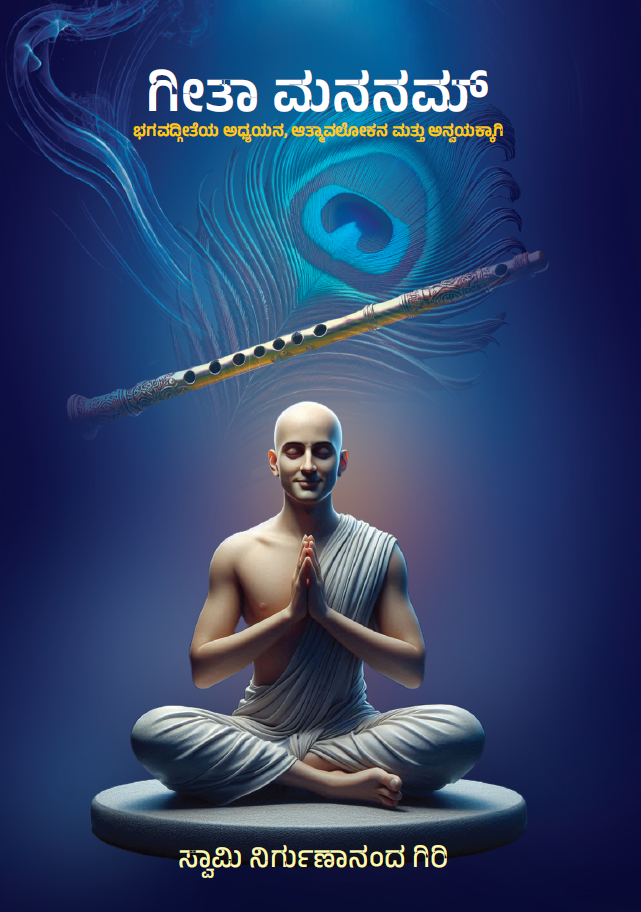
\includegraphics[width=\paperwidth,height=\paperheight]{./images/frontcover.png}%
    }%
}
    \begin{center}
        \vspace*{0.5cm}
            
        {\Huge
        %\textbf{\color{white}\fontsize{50}{60}\selectfont ಗೀತಾ ಮನನಂ}
		}
        %\textbf{\\ \small \color{white}ದೈನಂದಿನ ಸ್ಪೂರ್ತಿ ಹಾಗೂ ಆತ್ಮಾವಲೋಕನಕ್ಕಾಗಿ}    
        \vspace{1.0cm}
            
        
		
            
        \vfill
            
        
            
        \vspace{0.1cm}
        {\color{white}    
		%\textbf{{\Large \mananamfont ಸ್ವಾಮಿ ನಿರ್ಗುಣಾನಂದ ಗಿರಿ}}\\
		%{\normalsize Swami Nirgunananda Giri\\Rishikesh, India}
		}
    \end{center}
\end{titlepage}
\nopagecolor% Use this to restore the color pages to white
\begin{titlepage}
	%\pagecolor{pastelblue}
	%\AddToShipoutPictureBG*{%
    %\AtPageLowerLeft{%
    %    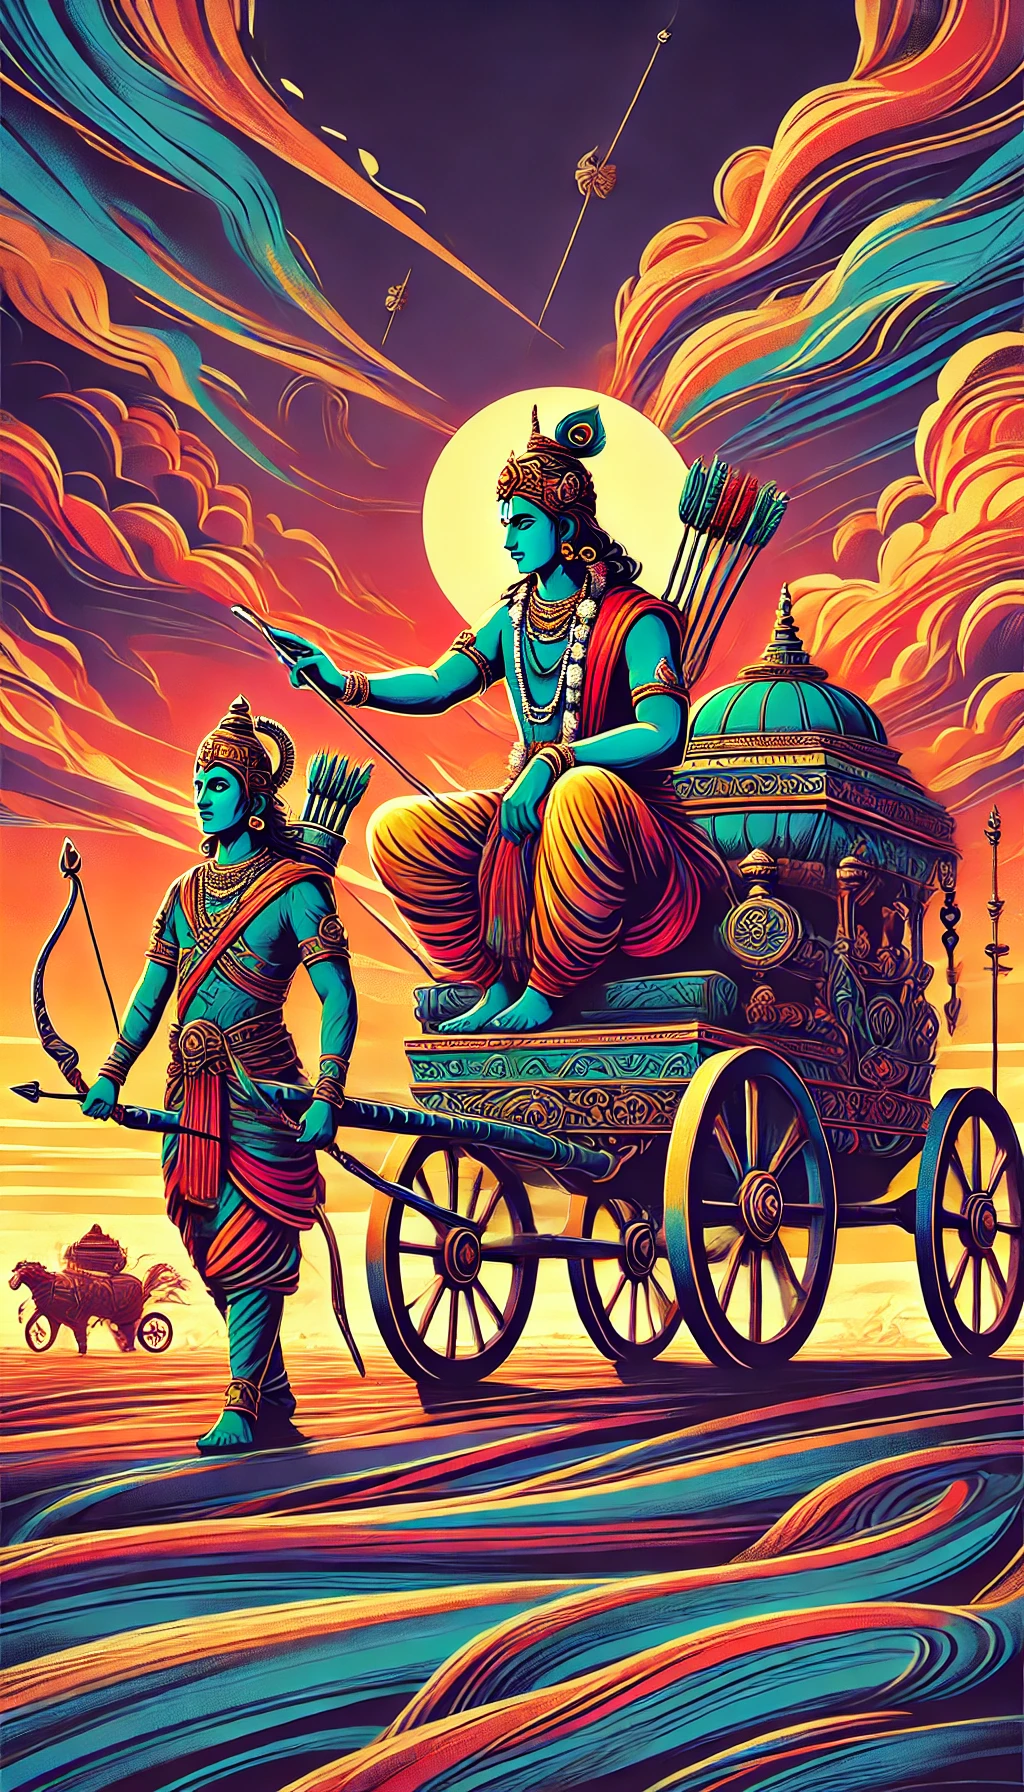
\includegraphics[width=\paperwidth,height=\paperheight]{./images/krishna4.jpg}%
    %}%
%}
    \begin{center}
        \vspace*{0.5cm}
            
        {\Huge
        \textbf{\color{blue}\fontsize{50}{60}\selectfont ಗೀತಾ ಮನನಂ}}
        \textbf{\\ \small \color{black}ದೈನಂದಿನ ಸ್ಪೂರ್ತಿ ಹಾಗೂ ಆತ್ಮಾವಲೋಕನಕ್ಕಾಗಿ}\\    
        \vspace{1.0cm}
		    \textbf{{\large \color{black} ಅಧ್ಯಾಯ ೫ ಕರ್ಮ ಸನ್ಯಾಸ ಯೋಗ}}\\		
        \vspace{6.0cm}
        \textbf{{\Large \color{blue}\mananamfont ಸ್ವಾಮಿ ನಿರ್ಗುಣಾನಂದ ಗಿರಿ}}\\    
        
		
            
        \vfill
            
        
            
        \vspace{0.1cm}
        {\color{black}    
		
		{{\large \color{blue}ಹೃಷೀಕೇಶ, ಉತ್ತರಾ ಖಂಡ}\\\normalsize ಭಾರತ}
        }
    \end{center}
\end{titlepage}
\nopagecolor% Use this to restore the color pages to white
%\maketitle

\thispagestyle{empty}
Copyright \textcopyright\ Swamy Nirgunanandagiri\\
\\
All rights reserved\\
\\
Edition - First, 2024\\
\vfill
Without written permission of the author it is forbidden to reproduce or adapt in any form or by any means any part of this  publication.\\
\\
Rishikesh, India\\
\newpage
\thispagestyle{empty}
\frontmatter

\doublespacing
\tableofcontents
\singlespacing
%\clearpage
%\newgeometry{margin=0pt} % Apply margin only for this page
%\thispagestyle{empty}
%\begin{center}
%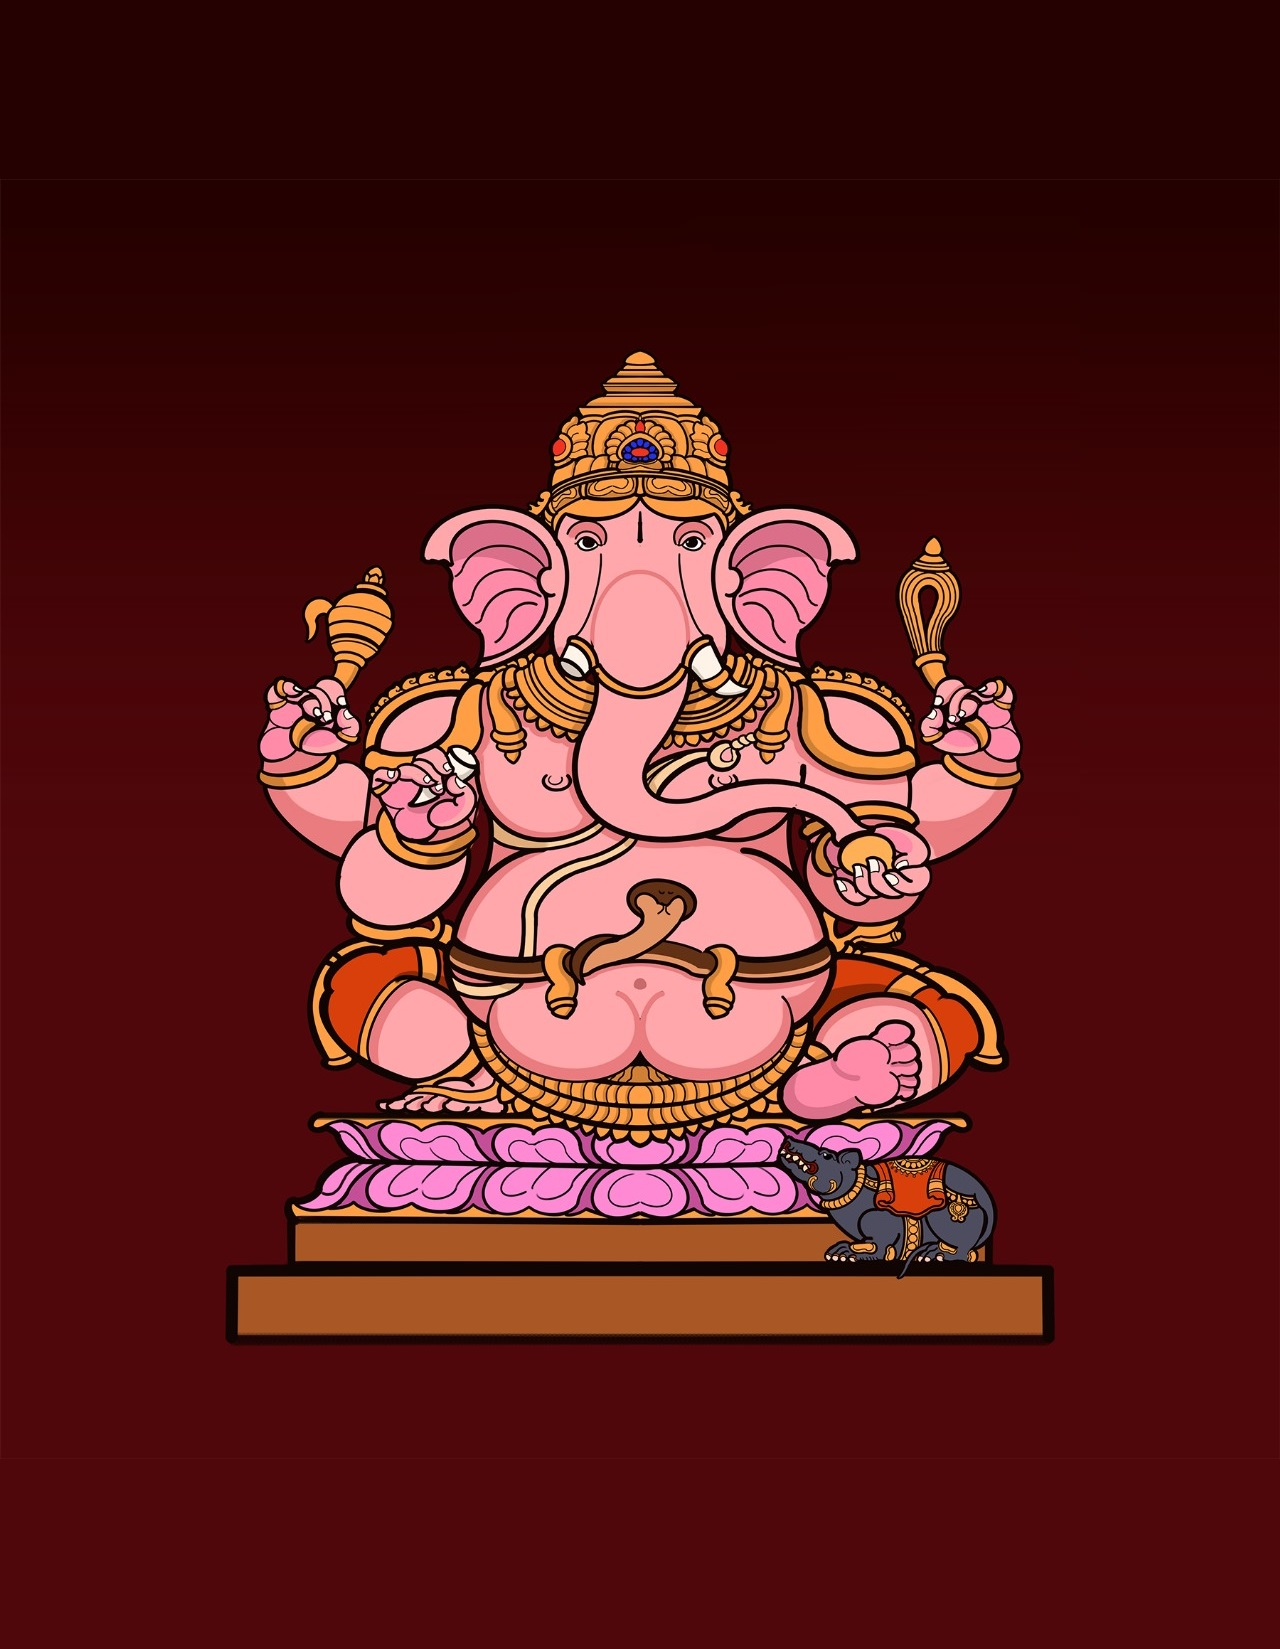
\includegraphics[width=0.9\textwidth, height=\paperheight, keepaspectratio]{./images/ganapa.jpg}
%\end{center}
%\restoregeometry % Restore original geometry settings
%\newpage

\clearpage
\newgeometry{margin=0pt} % Apply margin only for this page
\thispagestyle{empty}
%\begin{figure}
%\centering
%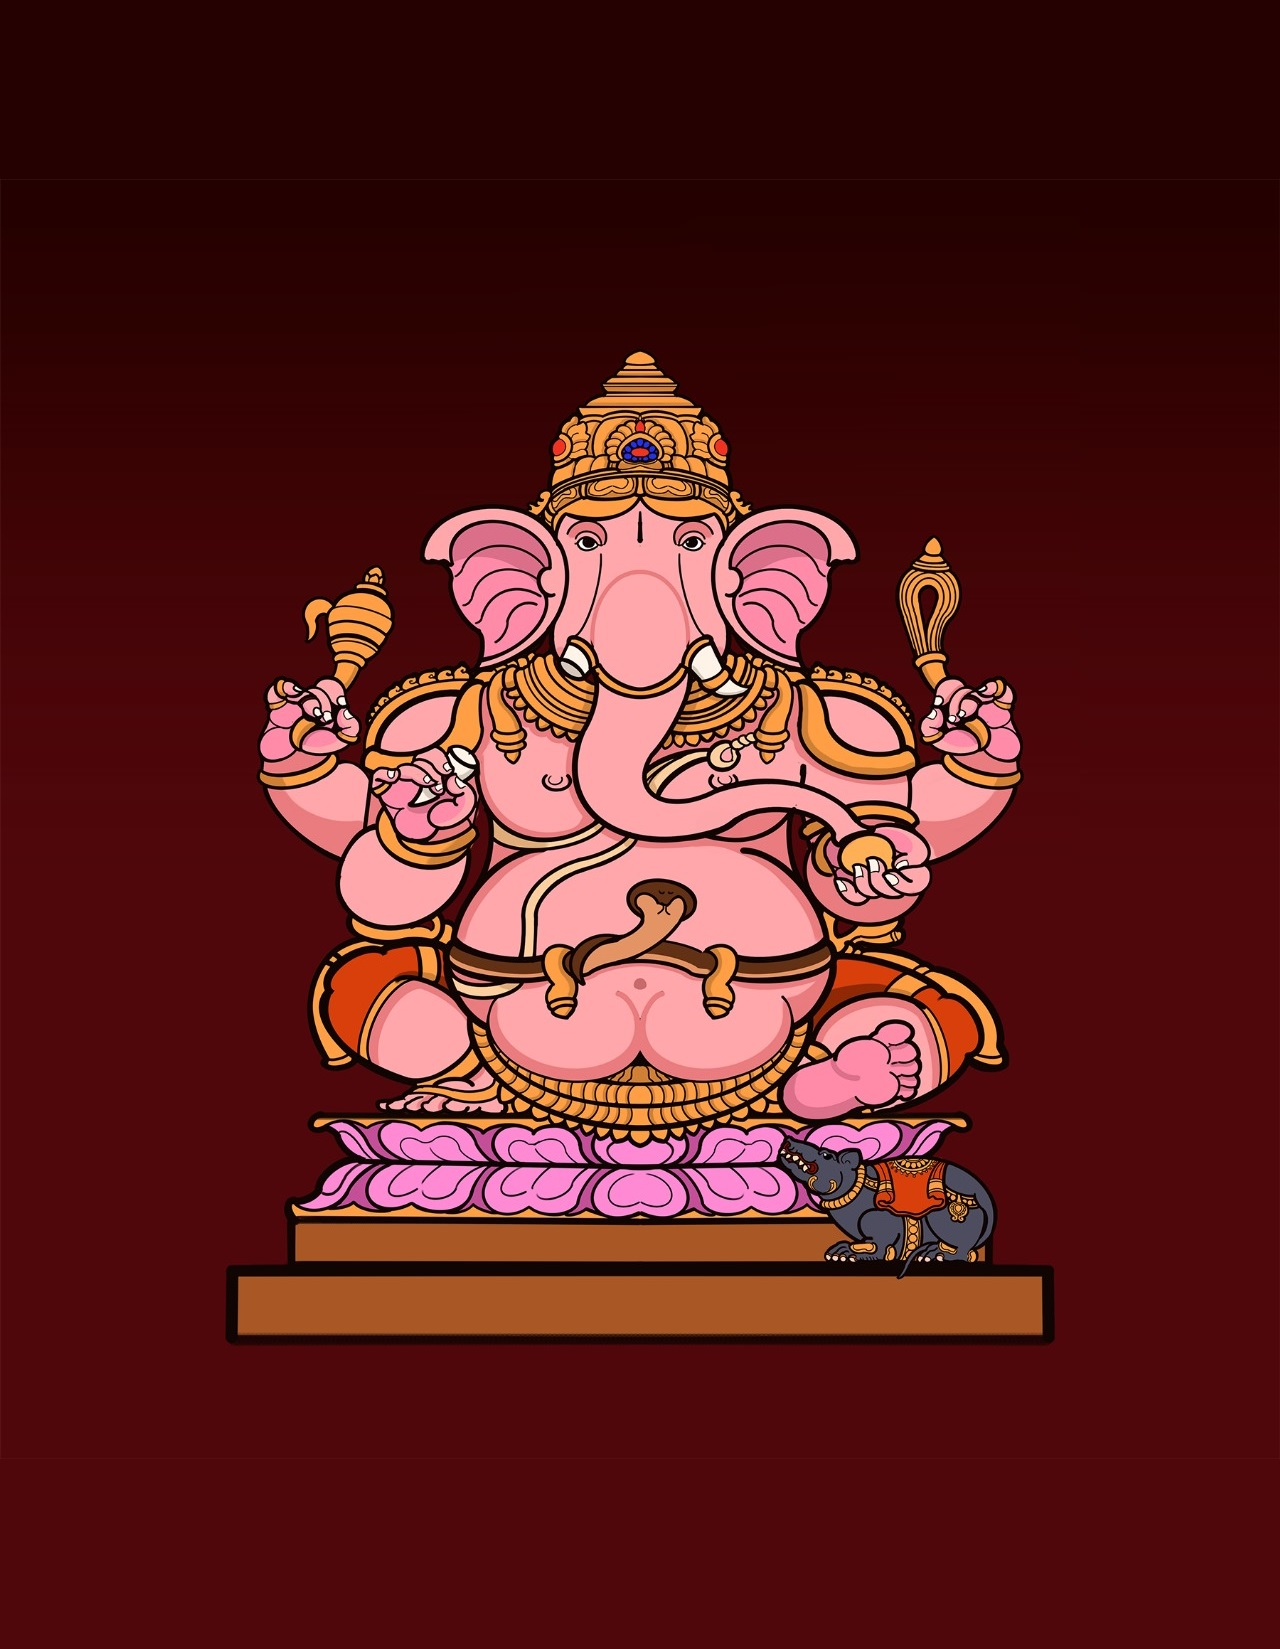
\includegraphics[width=0.9\textwidth, height=\paperheight, keepaspectratio]{./images/ganapa.jpg}
%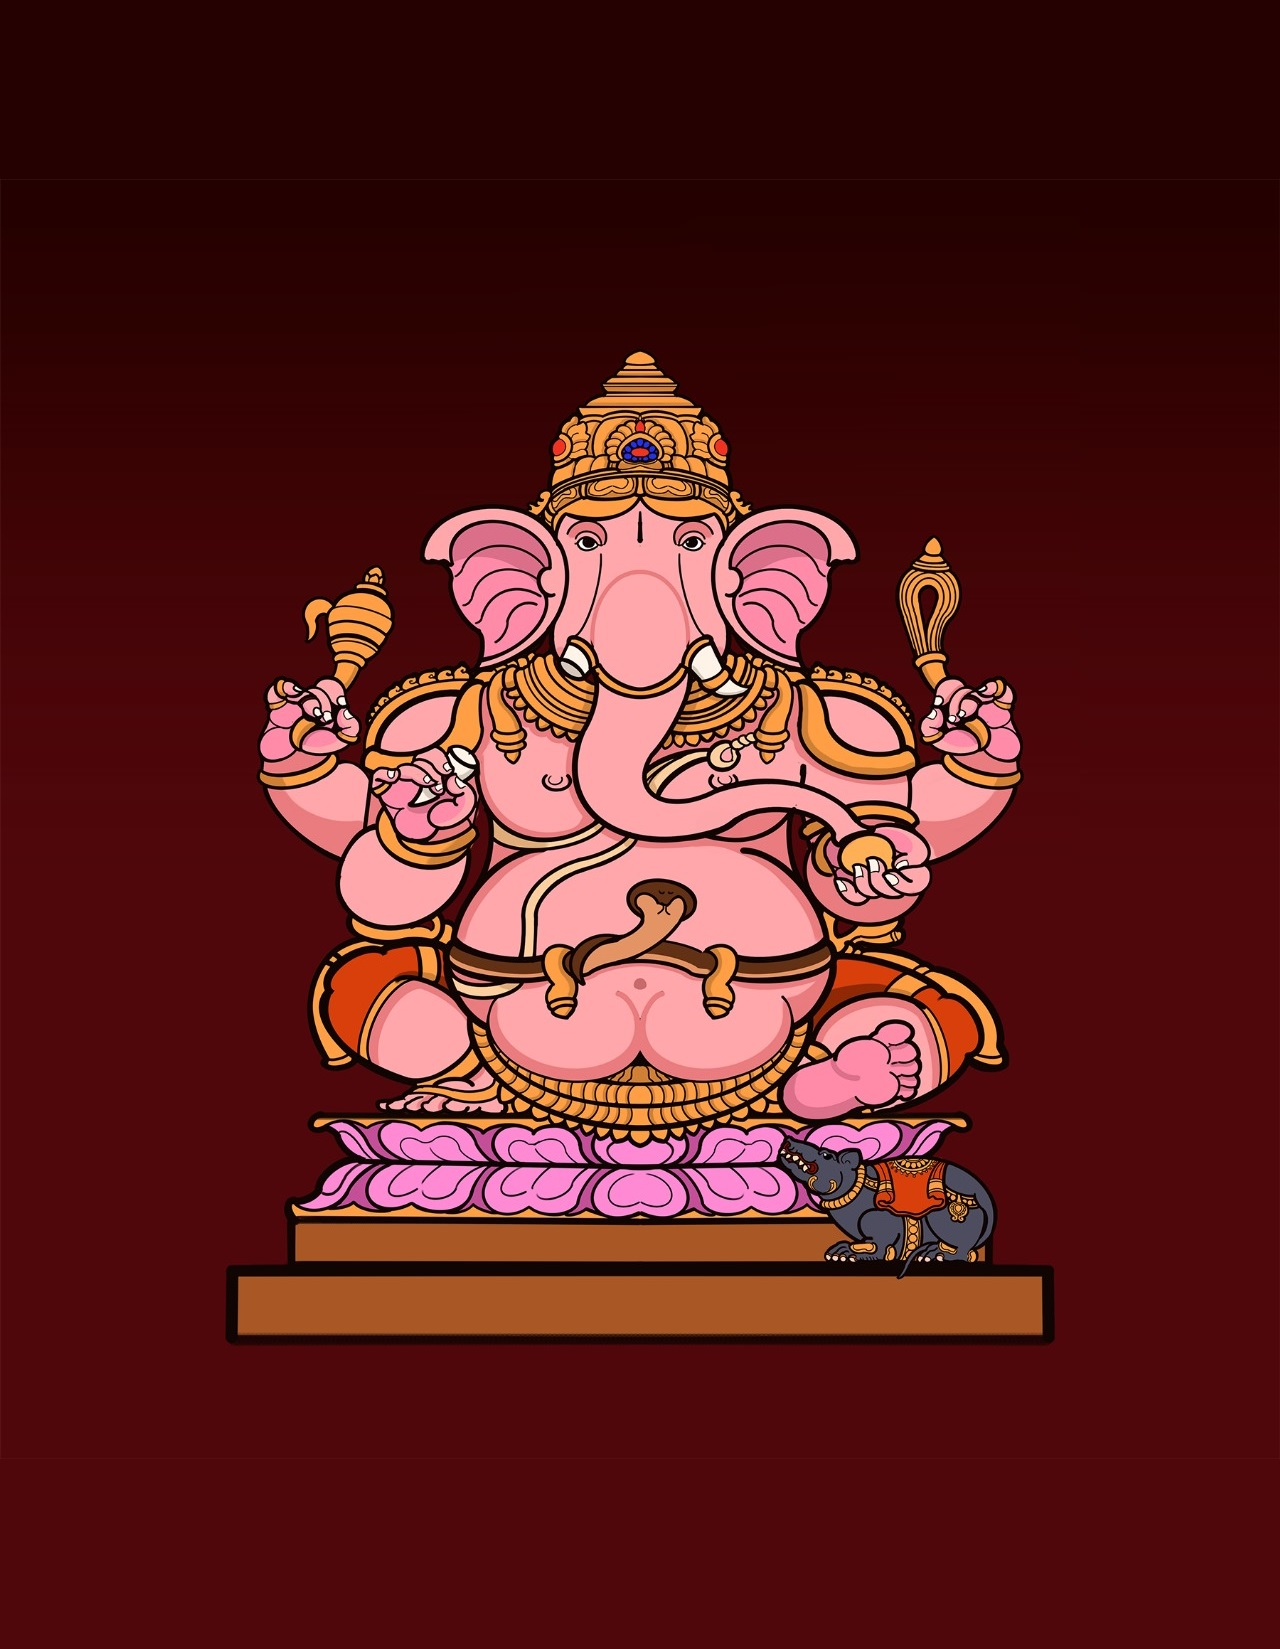
\includegraphics[width=\paperwidth, height=\paperheight]{./images/ganapa.jpg}
%\end{figure}
%\restoregeometry % Restore original geometry settings
%\newpage

\begin{figure}[h!]
    \centering
    \begin{overpic}[width=\paperwidth, height=\paperheight]{../images/001.jpg}
        \put(13,85){\color{white}\kanfont ಗಜಾನನಂ ಭೂತಗಣಾದಿ ಸೇವಿತಂ ಕಪಿತ್ಥ ಜಂಬೂಫಲಸಾರ ಭಕ್ಷಿತಮ್। }\put(10,82){\color{white}\kanfont ಉಮಾಸುತಂ ಶೋಕ ವಿನಾಶಕಾರಣಂ ನಮಾಮಿ ವಿಘ್ನೇಶ್ವರ ಪಾದಪಂಕಜಮ್॥ }
    \end{overpic}
    \caption{This is the standard figure caption below the image.}
    \label{fig:example}
\end{figure}

\restoregeometry

\thispagestyle{empty}
\thispagestyle{empty}
\pagestyle{fancy}


\chapter{\kanfont ಮುನ್ನುಡಿ}
\begin{center}
ದಿಶಂತು ಶಂ ಮೇ ಗುರುಪಾದಪಾಂಸವಃ ॥\\
\end{center}
\footnotesize \mananamtext{ಶ್ರಿ\!\char"0CD5ಮದ್ ಭಗವದ್ಗೀತೆಯು ಎಲ್ಲಾ ಧರ್ಮಗ್ರಂಥಗಳಲ್ಲಿ ಒಂದು ಅನನ್ಯ ಮತ್ತು ಸಾಟಿಯಿಲ್ಲದ ರತ್ನವಾಗಿದೆ.  ಇದು ಪರಿತ್ಯಾಗ ಮಾಡುವವರಿಗೆ ಮಾತ್ರವಲ್ಲದೆ ಲೌಕಿಕ ಜವಾಬ್ದಾರಿಗಳನ್ನು ಹೊತ್ತಿರುವವರಿಗೂ ಮಾರ್ಗದರ್ಶಿ ಬೆಳಕಾಗಿ ಕಾರ್ಯನಿರ್ವಹಿಸುತ್ತದೆ, ಆಧ್ಯಾತ್ಮಿಕದೊಂದಿಗೆ ಪ್ರಾಪಂಚಿಕತೆಯನ್ನು ಸಮತೋಲನಗೊಳಿಸಲು ಪ್ರಯತ್ನಿಸುತ್ತದೆ; ಇದು, ಅಜ್ಞಾನದಿಂದ ಅವರು (ಸಾಮಾನ್ಯ ಜನ) ತಮ್ಮನ್ನು ತಾವು,   ದೇಹ ಮತ್ತು ಮನಸ್ಸಿನ ವ್ಯವಹಾರಗಳ  ಜೊತೆ ಗುರುತಿಸಿಕೊಂಡಾಗ, ಅಂತಹ ವ್ಯವಹಾರಗಳ ಬಗ್ಗೆ ನಿಷ್ಪಕ್ಷಪಾತವಾಗಿರುವಂತೆ ಪ್ರತಿಪಾದಿಸುತ್ತದೆ.\\
ಜೀವನದಲ್ಲಿ ಒಬ್ಬರ ಕರ್ತವ್ಯಗಳನ್ನು ಸಾಧಿಸಲು, ಬಾಂಧವ್ಯದ ಅಥವಾ, ಮೋಹದ ಭಾವನೆ ಇರಬೇಕು ಎಂಬುದು ಒಂದು ತಪ್ಪು ಕಲ್ಪನೆ.  ಭಗವಾನ್ ಕೃಷ್ಣ, ಎಲ್ಲರಿಗಿಂತಲೂ  ದೊಡ್ಡ ಸಂಸಾರಿ ಹಾಗೂ, ಪರಿಪೂರ್ಣವಾದ ಮೋಹರಹಿತನಾದ ಅಸಂಸಾರಿ; ದಿವ್ಯವಾದ ಆನಂದದಲ್ಲಿ ನೆಲೆಗೊಂಡು, ಈ ಮೂರ್ತ, ಭೌತಿಕ ಜಗತ್ತಿನಲ್ಲಿ ಹೇಗೆ ಕಾರ್ಯನಿರ್ವಹಿಸಬೇಕು ಎಂಬುದನ್ನು ಅವನು ತನ್ನ ಕಾರ್ಯಗಳು, ಭಾವ ಮತ್ತು ಅವನು ಉಚ್ಛರಿಸುವ ಪ್ರತಿಯೊಂದೂ ಪರಮಪದದ  ಮೂಲಕ ಪ್ರದರ್ಶಿಸುತ್ತಾನೆ. ಆರಂಭದಲ್ಲಿ ‘ಸಂಘರ್ಷ ಮತ್ತು ಸವಾಲುಗಳಿಂದ ತುಂಬಿರುವ ಮಾರ್ಗ’ ಎಂದು ಕಂಡುಬoದರೂ ಸಹ, ಈ ಸ್ಥಿತಿಯನ್ನು ಸಾಧಿಸಲು (ದಿವ್ಯವಾದ ಆನಂದದಲ್ಲಿ ನೆಲೆಗೊಂಡು, ಈ ಮೂರ್ತ, ಭೌತಿಕ ಜಗತ್ತಿನಲ್ಲಿ  ಕಾರ್ಯನಿರ್ವಹಿಸುವುದು) ಸಮರ್ಥ ಶಿಕ್ಷಕರಿಂದ ಸರಿಯಾದ ಮಾರ್ಗದರ್ಶನದ ಅಗತ್ಯವಿದೆ. \\
ಈ ‘ನಿಪುಣ ಮಾರ್ಗದರ್ಶಿ ಕೈಪಿಡಿ’ಯಲ್ಲಿ, ಲೇಖಕರ ಆಳವಾದ ಒಳನೋಟದಿಂದ ಅಧ್ಯಾಯ 2 ರ 52-53 ಪದ್ಯಗಳಲ್ಲಿ ಸೂಚಿಸಿದಂತೆ: “ಶಿಕ್ಷಕರ ಮತ್ತು ಧರ್ಮಗ್ರಂಥಗಳ ಉದ್ದೇಶವು ನಮ್ಮನ್ನು ಭ್ರಮೆಯಿಂದ ಜಗ್ಗಿಸಿ, ಮುಕ್ತರನ್ನಾಗಿ ಮಾಡುವುದೇ ಆಗಿದೆ. ನಾವು ನಮ್ಮ ಲೌಕಿಕ ಚಿಂತನೆಯ ಮಾದರಿಗಳನ್ನು ಬಿಟ್ಟು, ಒಂದು ಉನ್ನತ ಸತ್ಯದಲ್ಲಿ (ಪಾರಮಾರ್ಥಿಕದಲ್ಲಿ) ಆಶ್ರಯ ಪಡೆಯಲು ಪ್ರಾರಂಭಿಸುತ್ತಿದ್ದಂತೆಯೇ, ಆಧ್ಯಾತ್ಮಿಕ ಪ್ರಯಾಣದ ಒಂದು ಭಾಗವಾದ ಗೊಂದಲಗಳು ಮತ್ತು ಸವಾಲುಗಳು ಏಳುತ್ತವೆ; ಆದರೆ, ನಾವು ಹೀಗೆ ಈ ಹಾದಿಯಲ್ಲಿ ಪ್ರಗತಿ ಹೊಂದುತ್ತಿದ್ದಂತೆ, ಸ್ಪಷ್ಟತೆ ಪಡೆಯಲು ಪ್ರಾರಂಭಿಸುತ್ತೇವೆ”.\\
ಈ ಪುಸ್ತಕವು ಲೇಖಕರ ಕ್ರಾಂತಿಕಾರಿ ಚಿಂತನೆಗಳ ಮೂಲಕ ಓದುಗರನ್ನು ದೇಹದಿಂದ, ಮನಸ್ಸಿಗೆ ಮತ್ತು ಮನಸ್ಸಿನಿಂದ ಪ್ರಜ್ಞೆಗೆ (ಚೈತನ್ಯಕ್ಕೆ), ಒಬ್ಬರ ಅಸ್ತಿತ್ವದ ಪದರಗಳನ್ನು ಭೇದಿಸುವಂತೆ ಮಾಡುತ್ತದೆ. \\
ಪ್ರತಿ ವಿಭಾಗದಲ್ಲಿ, ‘ಮನನಂ’ ಶೀರ್ಷಿಕೆಯಡಿಯಲ್ಲಿರುವ ಆತ್ಮಾವಲೋಕನದ ಪ್ರಶ್ನೆಗಳು, ಸ್ವಯಂ ಸಮಾಧಾನ ಮತ್ತು ಆತ್ಮವಂಚನೆಯಲ್ಲಿ (ಆತ್ಮ ಪ್ರವಂಚನ) ತೊಡಗಿರುವವರಿಗೆ ಯಾವುದೇ ವಿರಾಮ ನೀಡುವುದಿಲ್ಲ ಮತ್ತು ಪ್ರಾಮಾಣಿಕವಾದ ಸ್ವಯಂ ಮೌಲ್ಯಮಾಪನ ಮಾಡಲು ಅವರಿಗೆ ಸವಾಲು ಒಡ್ಡುತ್ತವೆ .  ಮತ್ತೊಂದೆಡೆ, ‘ಸ್ಫೂರ್ತಿ’ಯ ಅಡಿಯಲ್ಲಿರುವ ಪದಗಳು, ಪ್ರಯಾಸಕರ ಮತ್ತು ಗೊಂದಲಮಯ ಆಧ್ಯಾತ್ಮಿಕ ಮಾರ್ಗವನ್ನು ತುಲನಾತ್ಮಕವಾಗಿ ಸುಲಭಗೊಳಿಸಿ, ಸಕಾರಾತ್ಮಕತೆಯ ಒಂದು, ಅಕ್ಷಯವಾದ ಮೂಲವಾಗಿ ಕಾರ್ಯನಿರ್ವಹಿಸುತ್ತವೆ.\\
ಈ ಕೈಪಿಡಿಯು, ಆಕಾಂಕ್ಷಿಗಳಿಗೆ ಜೀವನದ ವಿವಿಧ ಸಮಸ್ಯೆಗಳಿಗೆ ಪರಿಹಾರವನ್ನು ಕಂಡುಕೊಳ್ಳಲು ಸಾಕಷ್ಟು ಸಮಾಧಾನಗಳನ್ನು  ನೀಡುತ್ತದೆ, ಆದರೆ ಬಾಹ್ಯವಾಗಿ ಅಲ್ಲ, ಆಂತರಿಕವಾಗಿ.\\
ಈ ಪುಸ್ತಕದ ವಿಷಯವು, ‘ಮಾನವ ಮನೋವಿಜ್ಞಾನ’ದ ಬಗ್ಗೆ ಲೇಖಕರ ಆಳವಾದ ತಿಳುವಳಿಕೆಯನ್ನು ತೋರಿಸುತ್ತದೆ, ಮೊದಲು ಸಕಾರಾತ್ಮಕ ಮಾನಸಿಕ ಸ್ಥಿತಿಯ ಕಡೆಗೆ ಮತ್ತು ನಂತರ ಅದನ್ನು ಮೀರಿ, ಆಂತರಿಕ ಶಾಶ್ವತವಾದ ಆತ್ಮದೆಡೆಗೆ, ಸರಳವಾಗಿ ಮುಂದುವರಿಯುತ್ತದೆ. \\
ಈ ಪುಸ್ತಕದ ಓದುಗರು ಈ ಪ್ರಯಾಣವನ್ನು ಪ್ರಾರಂಭಿಸಿದಾಗ, ಅವರು ಖಂಡಿತವಾಗಿಯೂ ಮಾನವ ಮನಸ್ಸಿನ ಕ್ಷೇತ್ರವನ್ನು ಮೀರುತ್ತಾರೆ ಮತ್ತು ಈ ಸ್ವರ್ಗೀಯ ಗೀತೆಯಾದ  ‘ಭಗವದ್ಗೀತೆ’ ಗಾಯಕನ ಕೃಪೆಯಿಂದ ‘ಅಧಿಷ್ಠಾನ ಚೈತನ್ಯಮ್’ (ಚೇತನಾತ್ಮಕದ ಅಂತಿಮ ಮೂಲತತ್ವ) ಅನ್ನು ತಲುಪುತ್ತಾರೆ. ಸಾಧಕರ ಅನುಕೂಲಕ್ಕಾಗಿ ತಮ್ಮ ಅಮೂಲ್ಯವಾದ ಆಲೋಚನೆಗಳನ್ನು ಲೇಖಿಸಿದ, ಸ್ವಾಮಿ ನಿರ್ಗುಣಾನಂದ ಗಿರಿ, ಇವರ ನಿಸ್ವಾರ್ಥ ಪ್ರಯತ್ನವನ್ನು,  ಸನಾತನ ಗುರುವಾದ, ಆ ಭಗವಂತ ಶ್ರೀಕೃಷ್ಣನು ಆಶೀರ್ವದಿಸಲಿ.\\\\
\begin{center}
ಮಂಗಳಂ ಸರ್ವಂ
\end{center}

{\kanBold ಸ್ವಾಮಿ ಸ್ವಾನಂದ ತೀರ್ಥ} \\
ಆಚಾರ್ಯ, ಕೈಲಾಸ್ ಆಶ್ರಮ\\
ಋಷಿಕೇಶ – ಉತ್ತರಖಂಡ\\
}
%\thispagestyle{empty}
\begin{onehalfspace}
\chapter{\kanfont ಪ್ರಸ್ತಾವನೆ}
\footnotesize \mananamtext{ನಾವೆಲ್ಲರೂ ಜೀವನದ ಹೋರಾಟಗಳನ್ನು ಎದುರಿಸಲೇಬೇಕು. ಕುರುಕ್ಷೇತ್ರ ಯುದ್ಧದಲ್ಲಿ ಶ್ರೀ ಕೃಷ್ಣ ಪರಮಾತ್ಮನು, ತನ್ನ ವೇದನಾಯುಕ್ತ ಶಿಷ್ಯ ಅರ್ಜುನನಿಗೆ, ಪ್ರಾಪಂಚಿಕತೆಯಲ್ಲಿಯೂ ಅಧ್ಯಾತ್ಮಿಕತೆಯನ್ನು ಆಚರಣೆಗೆ ತರುವಂತಹ, ಸಂಕ್ಷಿಪ್ತ ಹಾಗೂ ಪ್ರಾಯೋಗಿಕವಾದ,  ಅತೀ ಪವಿತ್ರವಾದ ಬೋಧನೆಗಳನ್ನು ಕೊಟ್ಟಿದ್ದಾನೆ. ಈ ಶ್ರೇಷ್ಠವಾದ ಉಪನಿಷತ್ತುಗಳ ಸತ್ವಗಳನ್ನೊಳಗೊಂಡ  ಬೋಧನೆಗಳನ್ನು ಪವಿತ್ರವಾದ, ‘ಭಗವದ್ಗೀತ, ಒಂದು ಪವಿತ್ರ ಗಾನ’ ದ ಸ್ವರೂಪದಲ್ಲಿ, ಋಷಿ ವೇದವ್ಯಾಸರು ನಮಗೆ ನೀಡಿರುವ ಅಸೀಮವಾದ ಕೊಡುಗೆ. \\
 ಅರ್ಜುನನು ಇದ್ದ ಪರಿಸ್ಥಿತಿಗೂ, ನಾವು ಇರುವ ಪರಿಸ್ಥಿತಿ ಮತ್ತು ಸಂಘರ್ಷಗಳಿಗೂ ವ್ಯತ್ಯಾಸಗಳಿರಬಹುದು. ಆದರೆ, ಗೀತೆಯ ಸಾರ್ವತ್ರಿಕ ಉಪದೇಶಗಳು ಸತ್ಯಾನ್ವೇಷಣೆ ಮಾಡಲು ಬಯಸುವ ಪ್ರತಿಯೊಬ್ಬನಿಗೂ ಆತ್ಮೋನ್ನತಿ  ಮತ್ತು ಅಧ್ಯಾತ್ಮಿಕ ಪ್ರಗತಿ ಸಾಧಿಸಲು ಬೇಕಾಗುವ ಮಾದರಿಯಾಗಿದೆ.\\
 ಭಗವದ್ಗೀತೆಯ ಉಪದೇಶಗಳು ಕೇವಲ ಆಧ್ಯಾತ್ಮಿಕ ಅನ್ವೇಷಣೆ ಮಾಡುವವರಿಗೆ ಸಮರ್ಪಿತವಾದದ್ದು ಮಾತ್ರವೇ ಅಲ್ಲ, ಜೀವನಕ್ಕೆ ಬೇಕಾಗುವ ಅತ್ಯಮೂಲ್ಯವಾದ ಕೈಪಿಡಿಯೂ ಆಗಿದೆ. ಯಾರು, ಕೆಲಸದಲ್ಲಿ ಮತ್ತು ಕೌಟುಂಬಿಕ ಜವಾಬ್ದಾರಿಗಳಲ್ಲಿ ಒತ್ತಡ ರಹಿತವಾಗಿ, ಸಮತೋಲನ ಮತ್ತು ಮಾನಸಿಕ ನೆಮ್ಮದಿ ಕಾಪಾಡಿಕೊಳ್ಳಲು  ಬಯಸುತ್ತಾರೋ ಅವರಿಗೆ ಈ ಬೋಧನೆಗಳು ಬಹಳ ಮಹತ್ವದ್ದಾಗಿರುತ್ತವೆ. \\
 ಅನೇಕ ಗುರುಗಳು ಮತ್ತು ವಿದ್ವಾಂಸರು ಈಗಾಗಲೇ ಮಾಡಿರುವಂತೆ ಈ ದಿನಚರಿ ಪುಸ್ತಕ ಮತ್ತು ನಿಯತಕಾಲಿಕವು, ಗೀತೆಯ ಬೋಧನೆಗಳನ್ನು ತಿಳಿಸುವ ಪ್ರಯತ್ನ ಅಥವಾ ವ್ಯಾಖ್ಯಾನ ಕೊಡುವುದಾಗಿಲ್ಲ. ಈ ಗೀತಾ ಮನನವು, ಬೋಧನೆಗಳ ಚಿಂತನೆ ಮಾಡುವುದು ಮತ್ತು ಅದನ್ನು ನಮ್ಮ ಸ್ವಂತದ್ದನ್ನಾಗಿ ಅಂದರೆ, ಜೀವನದಲ್ಲಿ ಅಳವಡಿಸಿಕೊಳ್ಳಲು ಸುಲಭವಾಗುವಂತೆ ಮಾಡಿಕೊಳ್ಳುವುದೇ ಆಗಿದೆ. ದೇವ ನಾಗರಿಯಲ್ಲಿರುವ `ಮನನ` ಎಂಬ ಪದವು ಆಗಲೇ ಕೇಳಿದ್ದನ್ನು ಅಥವಾ ಓದಿದ್ದನ್ನು ಚಿಂತನೆ ಮಾಡುವ ಕಾರ್ಯವಿಧಾನವನ್ನು ಅನ್ವಯಿಸುವುದಾಗಿದೆ.\\
 ಈ ದಿನಚರಿ ಪುಸ್ತಕವನ್ನು ನೀವು, ನಿಮ್ಮ ಮನಸ್ಸಿನ ಇಂಗಿತವನ್ನು ಸ್ವತಂತ್ರವಾಗಿ ವ್ಯಕ್ತಪಡಿಸಲು  ಮತ್ತು ನಿಮ್ಮ ಜೀವನದಲ್ಲಿ ಅಳವಡಿಸಿಕೊಳ್ಳಲು ಅವಕಾಶ ಮಾಡಿಕೊಡುವ ಸಲುವಾಗಿ  ರೂಪಿಸಲಾಗಿದೆ. ಗೀತೆಯಲ್ಲಿರುವ ಶ್ಲೋಕಗಳ ಆಧಾರದ ಮೇಲೆ ರಚಿಸಲಾಗಿರುವ ಈ ಪ್ರಶ್ನೆಗಳು, ಆಯಾ ಬೋಧನೆಗಳ ಸನ್ನಿವೇಶಕ್ಕೆ ತಕ್ಕಂತೆ, ನಿಮ್ಮ ವೈಯಕ್ತಿಕ ಅರ್ಥಗಳನ್ನು ಹುಡುಕಲು ಮತ್ತು ಅದರಿಂದ ಜೀವನದ ಸಂದರ್ಭದೊಳಗೆ ಅಪಾರ ಸ್ಪಷ್ಟನೆ ದೊರಕಿಸಲು ಸಹಾಯಕವಾಗುವಂತೆ ರೂಪಿಸಲಾಗಿದೆ.\\
 ಶ್ರಿ\!\char"0CD5ಕೃಷ್ಣ ಪರಮಾತ್ಮನು  ಅರ್ಜುನನಿಗೆ ಧಾರ್ಮಿಕ ಯುದ್ಧವನ್ನು ಮಾಡಲು ಪ್ರೇರೇಪಿಸಿದಂತೆ, ನಿಮ್ಮ ಜೀವನದ ದಿನನಿತ್ಯದ ಕರ್ತವ್ಯಗಳನ್ನು ಈ “ಗೀತಾ ಮನನಮ್ “ ಮೂಲಕ  ಸಮರ್ಪಕವಾಗಿ ನಿರ್ವಹಿಸಲು,  ಆ ಭಗವಂತ ನಿಮ್ಮನ್ನೂ ಪ್ರೇರೇಪಿಸುತ್ತಾನೆ ಎಂದು ನಂಬುತ್ತೇನೆ. ನಿಮ್ಮ ಅಂತರಂಗದ ಶಾಂತಿ, ವೈಯಕ್ತಿಕ ಪ್ರಗತಿಯನ್ನು ನಿರ್ಲಕ್ಷಿಸದೇ, ನಿಮ್ಮ ಕರ್ತವ್ಯಗಳನ್ನು ಕುಶಲತೆಯಿಂದ ಯಶಸ್ವಿಯಾಗಿ ನಿರ್ವಹಿಸುತ್ತಾ  ಮತ್ತು ನಿಶ್ಚಲವಾಗಿ ದೈವತ್ವದಲ್ಲಿ ಮನಸನ್ನಿಡುವುದೇ, ಈ ದಿವ್ಯವಾದ ಗೀತೆಯ ನಿರಂತರ ಉದ್ದೇಶ.\\
ನಾನು ಈ ಪುಸ್ತಕದಲ್ಲಿ ಬಳಸಿರುವ ಚಿತ್ರಕಲೆ ಮತ್ತು ರೇಖಾಚಿತ್ರಗಳಿಗಾಗಿ ಶ್ರಿ\!\char"0CD5ಯುತ ಕೆ.ಎಂ.ಶೇಷಗಿರಿ ಅವರಿಗೆ ಧನ್ಯವಾದಗಳನ್ನು ಸಲ್ಲಿಸುತ್ತೇನೆ. ನನ್ನ ಗೀತಾ ತರಗತಿಯಲ್ಲಿ ಭಾಗವಹಿಸಿದ್ದ ಅನೇಕ ವಿದ್ಯಾರ್ಥಿಗಳು ಶ್ಲೋಕಗಳ ಭಾಷಾಂತರ, ತಿದ್ದುವಿಕೆ, ಸಂಪಾದನೆ, ವಿನ್ಯಾಸ ಮತ್ತು ಮುದ್ರಣ ಪ್ರಕ್ರಿಯೆಯನ್ನು ಗಮನಿಸುವಲ್ಲಿ ತೊಡಗಿಸಿಕೊಂಡಿದ್ದಾರೆ. ಈ ಗ್ರಂಥವನ್ನು ಓದುಗರ ಹಿತಾರ್ಥಕ್ಕಾಗಿ ಸಮರ್ಪಣೆಯಿಂದ ಮಾಡಿದ ಅವರ ತ್ಯಾಗಮಯ ಸೇವೆಗೆ ಭಗವಂತನ ಕೃಪೆ ಹಾಗು ನನ್ನ ಆಶೀರ್ವಾದಗಳು. \\\\
}
{
\kanBold{ಸ್ವಾಮಿ ನಿರ್ಗುಣಾನಂದ ಗಿರಿ}
}

\end{onehalfspace}
\mainmatter
%\centerline{\textbf{ಅಥ ಪ್ರಥಮೋऽಧ್ಯಾಯಃ ।}\\}
ಮೊಟ್ಟ ಮೊದಲನೆಯ ಶ್ಲೋಕವೇ ನಮಗೆ ಚಿಂತನೆ, ಮನನ ಪ್ರಾರಂಭಿಸಲು ಬೇಕಾಗುವ ಸೂಕ್ಷ್ಮವಾದ ಸಂದೇಶವನ್ನು ಕೊಡುತ್ತದೆ.\\
\slcol{ಧೃತರಾಷ್ಟ್ರ ಉವಾಚ ।\\
\index{ಧರ್ಮಕ್ಷೇತ್ರೇ ಕುರುಕ್ಷೇತ್ರೇ} ಸಮವೇತಾ ಯುಯುತ್ಸವಃ ।\\
ಮಾಮಕಾಃ ಪಾಂಡವಾಶ್ಚೈವ ಕಿಮಕುರ್ವತ ಸಂಜಯ ॥ 1 ॥}
\cquote{ಧೃತರಾಷ್ಟ್ರನು ಹೇಳಿದನು,\\
ಸಂಜಯನೇ, ಯುದ್ಧದ ಬಯಕೆಯಿಂದ ಧರ್ಮಭೂಮಿಯಾದ ಕುರುಕ್ಷೇತ್ರದಲ್ಲಿ ಕಲೆತ ನನ್ನ ಮಕ್ಕಳೂ ಪಾಂಡವರೂ ಏನು ಮಾಡಿದರು?\\}
\slcol{ಸಂಜಯ ಉವಾಚ ।\\
\index{ದೃಷ್ಟ್ವಾ ತು ಪಾಂಡವಾನೀಕಂ} ವ್ಯೂಢಂ ದುರ್ಯೋಧನಸ್ತದಾ ।\\
ಆಚಾರ್ಯಮುಪಸಂಗಮ್ಯ ರಾಜಾ ವಚನಮಬ್ರವೀತ್ ॥ 2 ॥}
\cquote{ಸಂಜಯನು ಹೇಳಿದನು,\\
ಪಾಂಡವರ ದಂಡು ಸಜ್ಜಾಗಿ ನಿಂತಿದ್ದುದನ್ನು ನೋಡಿದ ಅರಸನಾದ ದುರ್ಯೋಧನನು ಗುರುಗಳಾದ ದ್ರೋಣರ ಬಳಿಗೆ ಬಂದು ಹೀಗೆ ಹೇಳಿದನು. \\}
\slcol{\index{ಪಶ್ಯೈತಾಂ ಪಾಂಡುಪುತ್ರಾಣಾಮಾಚಾರ್ಯ} ಮಹತೀಂ ಚಮೂಮ್ ।\\
ವ್ಯೂಢಾಂ ದ್ರುಪದಪುತ್ರೇಣ ತವ ಶಿಷ್ಯೇಣ ಧೀಮತಾ ॥ 3 ॥}
\cquote{ಗುರುಗಳೇ, ದೃಪದರಾಜನ ಮಗ ನಿಮ್ಮ ಶಿಷ್ಯ, ಬುದ್ಧಿಶಾಲಿಯಾದ ದೃಷ್ಟದ್ಯುಮ್ನ ಪಾಂಡವರ ಈ ದೊಡ್ಡ ದಂಡನ್ನು ಸಜ್ಜುಗೊಳಿಸಿರುವುದನ್ನು ನೋಡಿರಿ.\\}
\slcol{\index{ಅತ್ರ ಶೂರಾ ಮಹೇಷ್ವಾಸಾ} ಭೀಮಾರ್ಜುನಸಮಾ ಯುಧಿ ।\\
ಯುಯುಧಾನೋ ವಿರಾಟಶ್ಚ ದ್ರುಪದಶ್ಚ ಮಹಾರಥಃ ॥ 4 ॥}

\newpage
\begin{mananam}{\kanfont ಮನನ ಶ್ಲೋಕ - }
{\footnotesize \mananamfont ನನ್ನ ಜೀವನದ ದೈನಂದಿನ ನಿತ್ಯಕರ್ಮದಲ್ಲಿ ಯಾವಾಗ ನನ್ನ ದೇಹವು, ಆಸೆ, ಕೋಪ, ಭಯ, ಮತ್ಸರ ಇತ್ಯಾದಿಗಳಲ್ಲಿ ಒಲವು ತೋರುವುದನ್ನು ಗುರುತಿಸಿತು, ಅವುಗಳನ್ನು ಸ್ವಾತಂತ್ರ್ಯವನ್ನು ಆಳವಾಗಿ ಪ್ರೇರೇಪಿಸುವ ನನ್ನನ್ನು ಪ್ರತಿಭಟಿಸುವಂತೆ ಮಾಡುವ ಮತ್ತು ಸನಾತನ ಗ್ರಂಥ ಮತ್ತು ಬೋಧಕರಿಂದ ಪಡೆದ ಜ್ಞಾನವನ್ನು ಯಾವ ಬಲವನ್ನು ಅನುಸರಿಸಿದೆ? ನನ್ನ ಹಂಬಲ ಮತ್ತು ಸಂಕಲ್ಪಗಳನ್ನು ತಳ್ಳಿಹಾಕುವ ನನ್ನ ದುರಭ್ಯಾಸಗಳು ಮತ್ತು ಅಪಾಯಕಾರಿ ನಡವಳಿಕೆಗಳಿಂದಾಗಿ ನನ್ನ ನಿತ್ಯ ಜೀವನದಲ್ಲಿ ಏನೇನು ಕಷ್ಟ ಪಡಬೇಕಾಯಿತು?}
\end{mananam}
\WritingHand\enspace\textbf{ಆತ್ಮ ವಿಮರ್ಶೆ}
\begin{inspiration}{\kanfont ಸ್ಪೂರ್ತಿ}
{\footnotesize \mananamfont ನಿನಗೆ ನೀನು ಸತ್ಯವಾಗಿರು ಮತ್ತು ನೀನು ಉನ್ನತಿಯತ್ತ ಬದಲಾಗುವೆ. ಜೀವನದಲ್ಲಿ ಜಾಣನಿಗೆ ಅವಶ್ಯಕವಾದುದು ಪಕ್ಷಪಾತ ರಹಿತ ಅವಲೋಕನ. ನಮ್ಮನ್ನು ನಾವು ಬದಲಾಯಿಸಿಕೊಳ್ಳಲು ಕೇವಲ ಬಯಕೆ ಇದ್ದರೆ ಮಾತ್ರ ಸಾಲದು. ಜ್ಞಾನಿಗಳ ಮಹತ್ವದ, ಉನ್ನತವಾದ ಬೋಧನೆಗಳಿಂದ ನಮ್ಮ ಯೋಚನೆಗಳು, ಮಾತುಗಳು ಮತ್ತು ಕೃತಿಗಳನ್ನು ತಹಬಂದಿಗೆ ತಂದು, ಪ್ರತಿದಿನವೂ ನಮ್ಮನ್ನು ನಾವು ಆತ್ಮ ವಿಮರ್ಶೆ ಮಾಡಿಕೊಳ್ಳಲೇಬೇಕು.}
\end{inspiration}
\newpage

\cquote{ಈ ದಂಡಿನಲ್ಲಿ ಹೋರಾಟದಲ್ಲಿ ಭೀಮಾರ್ಜುನರಿಗೆ ಸರಿ ಜೋಡಿಯಾದ ಶೂರರಾಗಿ ದೊಡ್ಡ ದೊಡ್ಡ ಬಿಲ್ಲುಗಳನ್ನು ಹಿಡಿದುಕೊಂಡು ಕಾದುವುದರಲ್ಲಿ ಕುಶಲರಾದ ಸಾತ್ಯಕಿ ವಿರಾಟರಿದ್ದಾರೆ. ಸಹಸ್ರ ಜನರೊಡನೆ ಏಕಾಂಗಿಯಾಗಿ ಹೋರಾಡಬಲ್ಲ ದ್ರುಪದನಿದ್ದಾನೆ.\\}
\slcol{\index{ಧೃಷ್ಟಕೇತುಶ್ಚೇಕಿತಾನಃ} ಕಾಶಿರಾಜಶ್ಚ ವೀರ್ಯವಾನ್ ।\\
ಪುರುಜಿತ್ಕುಂತಿಭೋಜಶ್ಚ ಶೈಬ್ಯಶ್ಚ ನರಪುಂಗವಃ ॥ 5 ॥}
\cquote{ದೃಷ್ಟಕೇತು, ಚೀಕಿತಾನ, ವೀರನಾದ ಕಾಶಿರಾಜ, ಮತ್ತು ಮನುಷ್ಯರಲ್ಲಿ ಶ್ರೇಷ್ಠನಾದ ಶೈಭ್ಯ ಇವರೆಲ್ಲ ಇದ್ದಾರೆ. \\} 
\slcol{\index{ಯುಧಾಮನ್ಯುಶ್ಚ ವಿಕ್ರಾಂತ} ಉತ್ತಮೌಜಾಶ್ಚ ವೀರ್ಯವಾನ್ ।\\
ಸೌಭದ್ರೋ ದ್ರೌಪದೇಯಾಶ್ಚ ಸರ್ವ ಏವ ಮಹಾರಥಾಃ ॥ 6 ॥}
\cquote{ಬಲಶಾಲಿಯಾದ ಯುಧಾಮನ್ಯು, ವೀರನಾದ ಉತ್ತಮೌಜ, ಸುಭದ್ರೆಯ ಮಗ ಅಭಿಮನ್ಯು ಮತ್ತು ದ್ರೌಪದಿಯ ಮಕ್ಕಳು ಇದ್ದಾರೆ. ಎಲ್ಲರೂ ಒಬ್ಬೊಬ್ಬರು ಹತ್ತು ಸಹಸ್ರ ಜನರೊಡನೆ ಹೋರಾಡಬಲ್ಲ ಮಹಾರುತರು. \\}
\slcol{\index{ಅಸ್ಮಾಕಂ ತು ವಿಶಿಷ್ಟಾ ಯೇ} ತಾನ್ನಿಬೋಧ ದ್ವಿಜೋತ್ತಮ ।\\
ನಾಯಕಾ ಮಮ ಸೈನ್ಯಸ್ಯ ಸಂಙ್ಞಾರ್ಥಂ ತಾನ್ಬ್ರವೀಮಿ ತೇ ॥ 7 ॥}
\cquote{ಬ್ರಾಹ್ಮಣ ಶ್ರೇಷ್ಠರೇ, ನಮ್ಮ ಕಡೆಯಲ್ಲಿರುವ ವೀರರನ್ನು ನೆನಪಿಗೆ ತಂದುಕೊಳ್ಳಿ. ತಮಗೆ ನೆನಪಾಗಲೆಂದು ಅವರ ಹೆಸರುಗಳನ್ನು ಹೇಳುತ್ತೇನೆ.\\} 
\slcol{\index{ಭವಾನ್ಭೀಷ್ಮಶ್ಚ ಕರ್ಣಶ್ಚ} ಕೃಪಶ್ಚ ಸಮಿತಿಂಜಯಃ ।\\
ಅಶ್ವತ್ಥಾಮಾ ವಿಕರ್ಣಶ್ಚ ಸೌಮದತ್ತಿಸ್ತಥೈವ ಚ ॥ 8 ॥}
\cquote{ತಾವು ಭೀಷ್ಮ ಕರ್ಣ ಜಯಶೀಲನಾದ ಕೃಪಾ, ಅಶ್ವತ್ಥಾಮ, ವಿಕರ್ಣ ಸೋಮದತ್ತನ ಮಗನಾದ ಭೂರಿಶ್ರವ ಮತ್ತು ಜಯದ್ರಥ. \\}
\slcol{\index{ಅನ್ಯೇ ಚ ಬಹವಃ} ಶೂರಾ ಮದರ್ಥೇ ತ್ಯಕ್ತಜೀವಿತಾಃ ।\\
ನಾನಾಶಸ್ತ್ರಪ್ರಹರಣಾಃ ಸರ್ವೇ ಯುದ್ಧವಿಶಾರದಾಃ ॥ 9 ॥}
\cquote{ಇನ್ನೂ ಅನೇಕ ಶೂರರು ನನಗಾಗಿ ಜೀವ ತೆರಲು ಸಿದ್ದರಾಗಿ ಇದ್ದಾರೆ. ಎಲ್ಲರೂ ಎಲ್ಲ ಬಗಯ ಆಯುಧಗಳನ್ನು ಉಪಯೋಗಿಸಬಲ್ಲವರು ಮತ್ತು ಯುದ್ಧದಲ್ಲಿ ಗಟ್ಟಿಗರು.\\}
\slcol{\index{ಅಪರ್ಯಾಪ್ತಂ ತದಸ್ಮಾಕಂ} ಬಲಂ ಭೀಷ್ಮಾಭಿರಕ್ಷಿತಮ್ ।\\
ಪರ್ಯಾಪ್ತಂ ತ್ವಿದಮೇತೇಷಾಂ ಬಲಂ ಭೀಮಾಭಿರಕ್ಷಿತಮ್ ॥ 10 ॥}
\cquote{ಭೀಷ್ಮರ ರಕ್ಷಣೆಗೆ ಒಳಪಟ್ಟಿರುವ ನಮ್ಮ ದೊಡ್ಡ ಆ ದಂಡು ಸಾಲದೇನೋ ಎನಿಸುತ್ತದೆ. ಭೀಮನ ರಕ್ಷಣೆಗೆ ಒಳಪಟ್ಟಿರುವ ಪಾಂಡವರ ಈ ಸೇನೆ ಸಾಕಷ್ಟು ಸಮರ್ಥವಾಗಿದೆ.\\}
\slcol{\index{ಅಯನೇಷು ಚ ಸರ್ವೇಷು} ಯಥಾಭಾಗಮವಸ್ಥಿತಾಃ ।\\
ಭೀಷ್ಮಮೇವಾಭಿರಕ್ಷಂತು ಭವಂತಃ ಸರ್ವ ಏವ ಹಿ ॥ 11 ॥}
\cquote{ನೀವೆಲ್ಲರೂ ದಂಡಿನ ಬೇರೆ ಬೇರೆ ಮಾರ್ಗಗಳಲ್ಲಿ ನಿಮ್ಮ ನಿಮ್ಮ ಪಾಲಿಗೆ ಬಂದ ಕಡೆ ಇದ್ದುಕೊಂಡು ಭೀಷ್ಮನನ್ನು ರಕ್ಷಿಸಿರಿ.\\}
\slcol{\index{ತಸ್ಯ ಸಂಜನಯನ್ಹರ್ಷಂ} ಕುರುವೃದ್ಧಃ ಪಿತಾಮಹಃ ।\\
ಸಿಂಹನಾದಂ ವಿನದ್ಯೋಚ್ಚೈಃ ಶಂಖಂ ದಧ್ಮೌ ಪ್ರತಾಪವಾನ್ ॥ 12 ॥}
\cquote{ಹೀಗೆಂದು ಹೇಳಿದ ದುರ್ಯೋಧನನಿಗೆ ಹರ್ಷ ಉಂಟಾಗುವಂತೆ ಆಗ ಕುರುವಂಶದ ಹಿರಿಯ ಕೌರವರ ಅಜ್ಜ, ಪರಾಕ್ರಮಶಾಲಿ ಭೀಷ್ಮನು ಗಟ್ಟಿಯಾಗಿ ಸಿಂಹನಾದ ಮಾಡಿ ಶಂಖವನ್ನು ಊದಿದನು.\\}
\slcol{\index{ತತಃ ಶಂಖಾಶ್ಚ ಭೇರ್ಯಶ್ಚ} ಪಣವಾನಕಗೋಮುಖಾಃ ।\\
ಸಹಸೈವಾಭ್ಯಹನ್ಯಂತ ಸ ಶಬ್ದಸ್ತುಮುಲೋऽಭವತ್ ॥ 13 ॥}
\cquote{ಆಮೇಲೆ ಒಮ್ಮೆಲೆ ಶಂಖಗಳು, ಭೇರಿಗಳು, ಮೃದಂಗಗಳು, ನಗಾಡಿಗಳು, ರಣ ಸಿಂಹಗಳು ಒಳಗಿದವು. ಆ ಗದ್ದಲವು ಎಲ್ಲೆಲ್ಲಿಯೂ ತುಂಬಿತು.\\}
\slcol{\index{ತತಃ ಶ್ವೇತೈರ್ಹಯೈರ್ಯುಕ್ತೇ} ಮಹತಿ ಸ್ಯಂದನೇ ಸ್ಥಿತೌ ।\\
ಮಾಧವಃ ಪಾಂಡವಶ್ಚೈವ ದಿವ್ಯೌ ಶಂಖೌ ಪ್ರದಘ್ಮತುಃ ॥ 14 ॥}
\cquote{ಆಮೇಲೆ ಬಿಳಿ ಕುದುರೆಯನ್ನು ಹೂಡಿದ ದೊಡ್ಡ ತೇರಿನ ಮೇಲೆ ಕುಳಿತಿದ್ದ ಕೃಷ್ಣನೂ ಅರ್ಜುನನೂ ಹೆಸರುವಾಸಿಯಾದ ದಿವ್ಯವಾದ ತಮ್ಮ ಶಂಖಗಳನ್ನು ಊದಿದರು.\\}
\slcol{\index{ಪಾಂಚಜನ್ಯಂ ಹೃಷೀಕೇಶೋ} ದೇವದತ್ತಂ ಧನಂಜಯಃ ।\\
ಪೌಂಡ್ರಂ ದಧ್ಮೌ ಮಹಾಶಂಖಂ ಭೀಮಕರ್ಮಾ ವೃಕೋದರಃ ॥ 15 ॥}
\cquote{ಕೃಷ್ಣನು ಪಾಂಚಜನ್ಯವನ್ನೂ ಅರ್ಜುನನ್ನು ದೇವದತ್ತವನ್ನೂ, ಶತ್ರುಗಳನ್ನು ಎದೆಗೂಡಿಸುವ ಭೀಮನು ಪೌಂಡ್ರವೆಂಬ ದೊಡ್ಡ ಶಂಖವನ್ನು ಓದಿದನು.\\}
\slcol{\index{ಅನಂತವಿಜಯಂ ರಾಜಾ} ಕುಂತೀಪುತ್ರೋ ಯುಧಿಷ್ಠಿರಃ ।\\
ನಕುಲಃ ಸಹದೇವಶ್ಚ ಸುಘೋಷಮಣಿಪುಷ್ಪಕೌ ॥ 16 ॥}
\cquote{ಕುಂತಿಯ ಹಿರಿಯ ಮಗ, ಅರಸನಾದ ಧರ್ಮರಾಯನು ಅನಂತ ವಿಜಯವನ್ನೂ ನಕುಲನೂ ಸುಘೋಷವನ್ನೂ ಸಹದೇವನು ಮಣಿಪುಷ್ಪಕವನ್ನೂ ಊದಿದರು. \\}
\slcol{\index{ಕಾಶ್ಯಶ್ಚ ಪರಮೇಷ್ವಾಸಃ} ಶಿಖಂಡೀ ಚ ಮಹಾರಥಃ ।\\
ಧೃಷ್ಟದ್ಯುಮ್ನೋ ವಿರಾಟಶ್ಚ ಸಾತ್ಯಕಿಶ್ಚಾಪರಾಜಿತಃ ॥ 17 ॥\\
\index{ದ್ರುಪದೋ ದ್ರೌಪದೇಯಾಶ್ಚ} ಸರ್ವಶಃ ಪೃಥಿವೀಪತೇ ।\\
ಸೌಭದ್ರಶ್ಚ ಮಹಾಬಾಹುಃ ಶಂಖಾಂದಧ್ಮುಃ ಪೃಥಕ್ಪೃಥಕ್ ॥ 18 ॥}
\cquote{ಓ ಧೃತರಾಷ್ಟ್ರ ಕೇಳು, ಹಿರಿಯ ಬಿಲ್ಲೋಜ ಕಾಶಿರಾಜ, ಮಹಾರಥನಾದ ಶಿಖಂಡಿ, ಧೃಷ್ಟದ್ಯುಮ್ನ,  ವಿರಾಟ, ಸೋಲರಿಯದ ಸಾತ್ಯಕಿ, ದ್ರುಪದ, ದ್ರೌಪದಿಯ ಮಕ್ಕಳು, ಮಹಾಬಾಹುವಾದ ಅಭಿಮನ್ಯು ಹೀಗೆ ಎಲ್ಲರೂ ತಮ್ಮ ತಮ್ಮ ಶಂಖಗಳನ್ನು ಊದಿದರು.\\}
\slcol{\index{ಸ ಘೋಷೋ ಧಾರ್ತರಾಷ್ಟ್ರಾಣಾಂ} ಹೃದಯಾನಿ ವ್ಯದಾರಯತ್ ।\\
ನಭಶ್ಚ ಪೃಥಿವೀಂ ಚೈವ ತುಮುಲೋ ವ್ಯನುನಾದಯನ್ ॥ 19 ॥}
\cquote{ಆ ಗದ್ದಲವು ಭೂಮಿಯಲ್ಲಿಯೂ ಆಕಾಶದಲ್ಲಿಯೂ ತುಂಬಿ ಪ್ರತಿಧ್ವನಿಯನ್ನು ಹಬ್ಬಿಸಿ ಕೌರವರ ಎದೆ ಬಿರಿಯುವಂತೆ ಮಾಡಿತು.\\}
\slcol{\index{ಅಥ ವ್ಯವಸ್ಥಿತಾಂದೃಷ್ಟ್ವಾ} ಧಾರ್ತರಾಷ್ಟ್ರಾನ್ಕಪಿಧ್ವಜಃ ।\\
ಪ್ರವೃತ್ತೇ ಶಸ್ತ್ರಸಂಪಾತೇ ಧನುರುದ್ಯಮ್ಯ ಪಾಂಡವಃ ॥ 20 ॥\\
\index{ಹೃಷೀಕೇಶಂ ತದಾ} ವಾಕ್ಯಮಿದಮಾಹ ಮಹೀಪತೇ ।}
\cquote{ಓ ಧೃತರಾಷ್ಟ್ರ, ಸಜ್ಜಾಗಿ ಎದುರಿಗೆ ನಿಂತಿರುವ ಕೌರವರನ್ನು ನೋಡಿ ಕಪಿಧ್ವಜನಾದ ಅರ್ಜುನನು ಹೊಡೆದಾಟಕ್ಕೆ ಮೊದಲು ಮಾಡಬೇಕಾದ ಆ ಸಮಯದಲ್ಲಿ ಗಾಂಡೀವವನ್ನು ಕೈಗೆ ತೆಗೆದುಕೊಂಡು ಕೃಷ್ಣನನ್ನು ಕುರಿತು ಈ ಮಾತನ್ನು ಹೇಳಿದನು.\\}
\slcol{ಅರ್ಜುನ ಉವಾಚ ।\\
ಸೇನಯೋರುಭಯೋರ್ಮಧ್ಯೇ ರಥಂ ಸ್ಥಾಪಯ ಮೇऽಚ್ಯುತ ॥ 21 ॥}
\cquote{ಅರ್ಜುನನ್ನು ಹೇಳಿದನು, ಕೃಷ್ಣ, ಎರಡು ದಂಡುಗಳ ನಡುವೆ ನನ್ನ ರಥವನ್ನು ನಿಲ್ಲಿಸು.\\}
\slcol{\index{ಯಾವದೇತಾನ್ನಿರೀಕ್ಷೇऽಹಂ} ಯೋದ್ಧುಕಾಮಾನವಸ್ಥಿತಾನ್ ।\\
ಕೈರ್ಮಯಾ ಸಹ ಯೋದ್ಧವ್ಯಮಸ್ಮಿನ್ರಣಸಮುದ್ಯಮೇ ॥ 22 ॥}
\cquote{ಕಾದಬೇಕೆಂದು ನಿಂತಿರುವವರನ್ನು, ಈ ಯುದ್ಧದಲ್ಲಿ ನಾನು ಯಾರೊಡನೆ ಕಾದಬೇಕಾಗಿದೆ ಎಂಬುದನ್ನು ಒಮ್ಮೆ ನೋಡುತ್ತೇನೆ.\\}
\slcol{\index{ಯೋತ್ಸ್ಯಮಾನಾನವೇಕ್ಷೇऽಹಂ} ಯ ಏತೇऽತ್ರ ಸಮಾಗತಾಃ ।\\
ಧಾರ್ತರಾಷ್ಟ್ರಸ್ಯ ದುರ್ಬುದ್ಧೇರ್ಯುದ್ಧೇ ಪ್ರಿಯಚಿಕೀರ್ಷವಃ ॥ 23 ॥}
\cquote{ದುರ್ಬುದ್ಧಿಯ ದುರ್ಯೋಧನನಿಗೆ ಈ ಯುದ್ಧದಲ್ಲಿ ನೆರವಾಗಬೇಕೆಂದು ಕಾದುವುದಕ್ಕಾಗಿ ಯಾರು ಯಾರು ಇಲ್ಲಿಗೆ ಬಂದಿರುತ್ತಾರೆ ಎಂಬುದನ್ನು ನಾನೊಮ್ಮೆ ನೋಡುತ್ತೇನೆ.\\}
\slcol{ಸಂಜಯ ಉವಾಚ ।\\
\index{ಏವಮುಕ್ತೋ ಹೃಷೀಕೇಶೋ} ಗುಡಾಕೇಶೇನ ಭಾರತ ।\\
ಸೇನಯೋರುಭಯೋರ್ಮಧ್ಯೇ ಸ್ಥಾಪಯಿತ್ವಾ ರಥೋತ್ತಮಮ್ ॥ 24 ॥\\
\index{ಭೀಷ್ಮದ್ರೋಣಪ್ರಮುಖತಃ} ಸರ್ವೇಷಾಂ ಚ ಮಹೀಕ್ಷಿತಾಮ್ ।\\
ಉವಾಚ ಪಾರ್ಥ ಪಶ್ಯೈತಾನ್ಸಮವೇತಾನ್ಕುರೂನಿತಿ ॥ 25 ॥}
\cquote{ಸಂಜಯನು ಹೇಳಿದನು,\\
ಧೃತರಾಷ್ಟ್ರನೇ, ಅರ್ಜುನನು ಹೀಗೆ ಹೇಳಿದಾಗ ಕೃಷ್ಣನು ಭೀಷ್ಮ ದ್ರೋಣರ ಮತ್ತು ಎಲ್ಲಾ ಅರಸರ ಎದುರಿಗೆ ಎರಡು ದಂಡುಗಳ ನಡುವೆ ರಥವನ್ನು ನಿಲ್ಲಿಸಿ ‘ಅರ್ಜುನನೇ ಇಲ್ಲಿ ನೆರೆದಿರುವರನ್ನು ನೋಡು’ ಎಂದು ಹೇಳಿದನು.\\}
\slcol{\index{ತತ್ರಾಪಶ್ಯತ್ಸ್ಥಿತಾನ್ಪಾರ್ಥಃ} ಪಿತೂನಥ ಪಿತಾಮಹಾನ್ ।\\
ಆಚಾರ್ಯಾನ್ಮಾತುಲಾನ್ಭ್ರಾತೂನ್ಪುತ್ರಾನ್ಪೌತ್ರಾನ್ಸಖೀಂಸ್ತಥಾ ॥ 26 ॥}
\cquote{ಅರ್ಜುನು ಅಲ್ಲಿ ನಿಂತಿರುವ ಪಿತೃತುಲ್ಯರು, ಅಜ್ಜಂದಿರು, ಗುರುಗಳು, ಸೋದರ ಮಾವಂದಿರು, ಅಣ್ಣತಮ್ಮಂದಿರು, ಮಕ್ಕಳು, ಮೊಮ್ಮಕ್ಕಳು, ಜೊತೆಗಾರರು, ಮಾವಂದಿರು, ಸ್ನೇಹಿತರು- ಹೀಗೆ ಎಲ್ಲ ಬಗೆಯ ಬಂಧುಗಳನ್ನು ಎರಡು ಕಡೆಯ ದಂಡಿನಲ್ಲಿ ಕಂಡನು.\\}
\slcol{\index{ಶ್ವಶುರಾನ್ಸುಹೃದಶ್ಚೈವ} ಸೇನಯೋರುಭಯೋರಪಿ ।\\
ತಾನ್ಸಮೀಕ್ಷ್ಯ ಸ ಕೌಂತೇಯಃ ಸರ್ವಾನ್ಬಂಧೂನವಸ್ಥಿತಾನ್ ॥ 27 ॥}
\cquote{ಹೀಗೆ ಅಲ್ಲಿ ನೆರೆದಿರುವ ಬಂಧುಗಳನ್ನೆಲ್ಲ ನೋಡಿ ಅರ್ಜುನನು ತುಂಬಾ ಕನಿಕರಗೊಂಡು ವಿಷಾದದಿಂದ ಈ ಮಾತನ್ನು ಹೇಳಿದನು.\\}
\slcol{\index{ಕೃಪಯಾ ಪರಯಾವಿಷ್ಟೋ} ವಿಷೀದನ್ನಿದಮಬ್ರವೀತ್ ।\\
ಅರ್ಜುನ ಉವಾಚ ।\\
ದೃಷ್ಟ್ವೇಮಂ ಸ್ವಜನಂ ಕೃಷ್ಣ ಯುಯುತ್ಸುಂ ಸಮುಪಸ್ಥಿತಮ್ ॥ 28 ॥\\
\index{ಸೀದಂತಿ ಮಮ ಗಾತ್ರಾಣಿ} ಮುಖಂ ಚ ಪರಿಶುಷ್ಯತಿ ।\\
ವೇಪಥುಶ್ಚ ಶರೀರೇ ಮೇ ರೋಮಹರ್ಷಶ್ಚ ಜಾಯತೇ ॥ 29 ॥}
\cquote{ಅರ್ಜುನನು ಹೇಳಿದನು,\\
ಕೃಷ್ಣ, ಕಾದುವುದಕೆಂದು ನೆರೆದಿರುವ ಈ ನನ್ನವರನ್ನು ನೋಡಿ ನನ್ನ ಅವಯವಗಳು ಸೊರುಗುತ್ತಿವೆ. ಬಾಯಿ ಒಣಗುತ್ತಿದೆ. ನನ್ನ ಮೈಯಲ್ಲಿ ನಡುಕ ಮೂಡಿ ರೋಮ ನಿಗುರಿ ನಿಂತಿದೆ.\\}
\slcol{\index{ಗಾಂಡೀವಂ ಸ್ರಂಸತೇ} ಹಸ್ತಾತ್ತ್ವಕ್ಚೈವ ಪರಿದಹ್ಯತೇ ।\\
ನ ಚ ಶಕ್ನೋಮ್ಯವಸ್ಥಾತುಂ ಭ್ರಮತೀವ ಚ ಮೇ ಮನಃ ॥ 30 ॥}
\cquote{ಕೈಯಿಂದ ಗಾಂಡೀವ ಧನುಸ್ಸು ಕುಸಿಯುತ್ತಿದೆ. ಚರ್ಮವು ಸುಡುತ್ತಿದೆ. ನನಗೆ ನಿಲ್ಲುವುದಕ್ಕೂ ಆಗುವುದಿಲ್ಲ. ನನ್ನ ಮನಸ್ಸು ತಳಮಳಗೊಂಡಿದೆ.\\}
\slcol{\index{ನಿಮಿತ್ತಾನಿ ಚ ಪಶ್ಯಾಮಿ} ವಿಪರೀತಾನಿ ಕೇಶವ ।\\
ನ ಚ ಶ್ರೇಯೋऽನುಪಶ್ಯಾಮಿ ಹತ್ವಾ ಸ್ವಜನಮಾಹವೇ ॥ 31 ॥}
\cquote{ಕೃಷ್ಣ, ಕೆಟ್ಟ ಅಪಶಕುನಗಳನ್ನು ಕಾಣುತ್ತಿದ್ದೇನೆ. ಯುದ್ಧದಲ್ಲಿ ನನ್ನವರನ್ನು ಕೊಂದರೆ ಒಳ್ಳೆಯದಾದೀತೆಂದು ನನಗೆ ಅನ್ನಿಸುವುದಿಲ್ಲ.\\}
\slcol{\index{ನ ಕಾಂಕ್ಷೇ ವಿಜಯಂ ಕೃಷ್ಣ} ನ ಚ ರಾಜ್ಯಂ ಸುಖಾನಿ ಚ ।\\
ಕಿಂ ನೋ ರಾಜ್ಯೇನ ಗೋವಿಂದ ಕಿಂ ಭೋಗೈರ್ಜೀವಿತೇನ ವಾ ॥ 32 ॥}
\cquote{ಕೃಷ್ಣ, ನನಗೆ ಗೆಲ್ಲುವ ಬಯಕೆ ಇಲ್ಲ. ನನಗೆ ರಾಜ್ಯವು ಬೇಡ, ಸುಖಗಳೂ ಬೇಡ. ಗೋವಿಂದ, ಇಂಥ ರಾಜ್ಯದಿಂದಾಗಲಿ ಭೋಗದಿಂದಾಗಲಿ ಬದುಕಿನಿಂದಲೆ ಆಗಲಿ ಏನು ಪ್ರಯೋಜನ?\\}

\newpage
\begin{mananam}{\kanfont ಮನನ  ಶ್ಲೋಕ - \textenglish{28,29,30}}
{\footnotesize \mananamfont ನನ್ನ ಜೀವನದಲ್ಲಿ ಎದುರಿಸಿದ ಭಯಂಕರವಾದ ಉದ್ವೇಗಗಳನ್ನು ಎದುರಿಸಬೇಕಾದ ಸಂದರ್ಭದಲ್ಲಿ ಪರ್ಯಾಲೋಚಿಸುತ್ತೇವೆ. ಮತ್ತು ಹೊರಗಿನ ಸನ್ನಿವೇಶಗಳಿಂದಾಗಿ ನನ್ನೊಳಗೆ ಮಿತಿಮೀರಿದವು ಇರುವಂತಾಯಿತು.ಜೀವನದ ಅಂತಹ ಸಂದರ್ಭಗಳಲ್ಲಿ ನನ್ನ ಮಾನಸಿಕ ಭಯಗಳಿಂದಾಗಿ ನನ್ನ ದೈಹಿಕ ಸ್ಥಿತಿ ಕುಂಟಿತ ವಾಯಿತೆಂಬುದನ್ನು ನಾನು ಅರಿತಿದ್ದೇನೆಯೇ? ನಾನು ನನ್ನ ಜೀವನದಲ್ಲಿನ ಉದ್ವೇಗ ಮತ್ತು ಭಯವನ್ನು ಹೇಗೆ ಎದುರಿಸಲಿ?}
\end{mananam}
\WritingHand\enspace\textbf{ಆತ್ಮ ವಿಮರ್ಶೆ}
\begin{inspiration}{\kanfont ಸ್ಪೂರ್ತಿ}
{\footnotesize \mananamfont ನಿಮ್ಮ ಯೋಚನೆಗಳ ಬಗ್ಗೆ ಎಚ್ಚರ ವಹಿಸಬೇಕು.ನಿಮ್ಮ ಮಾನಸಿಕ ಸ್ಥಿತಿ ನಿಮ್ಮ ದೇಹದ ಮೇಲೆ ಪರಿಣಾಮ ಬೀರುತ್ತದೆ. ಪ್ರತಿನಿತ್ಯದ ಒತ್ತಡದಿಂದ ಮನಸ್ಸನ್ನು ಸ್ವಾತಂತ್ರ್ಯಗೊಳಿಸಲು ಕೆಲವು ಸರಳ ಯೋಗದ ಮತ್ತು ಉಸಿರಾಟದ ಪ್ರಕ್ರಿಯೆಗಳು ಸಹಕಾರಿಯಾಗುತ್ತವೆ.}
\end{inspiration}
\newpage

\slcol{\index{ಯೇಷಾಮರ್ಥೇ ಕಾಂಕ್ಷಿತಂ} ನೋ ರಾಜ್ಯಂ ಭೋಗಾಃ ಸುಖಾನಿ ಚ ।\\
ತ ಇಮೇऽವಸ್ಥಿತಾ ಯುದ್ಧೇ ಪ್ರಾಣಾಂಸ್ತ್ಯಕ್ತ್ವಾ ಧನಾನಿ ಚ ॥ 33 ॥}
\cquote{ಯಾರಿಗಾಗಿ ನಾವು ರಾಜ್ಯವನ್ನೂ ಭೋಗಗಳನ್ನೂ ಸುಖಗಳನ್ನೂ ಬಯಸಿದೆವೋ, ಆ ಜನರೆಲ್ಲ ಜೀವದಾಸೆಯನ್ನೂ ಸಿರಿಯನ್ನೂ ತೊರೆದು ಇಲ್ಲಿ ಕಾದುವುದಕ್ಕೆ ನಿಂತಿದ್ದಾರೆ.\\}
\slcol{\index{ಆಚಾರ್ಯಾಃ ಪಿತರಃ} ಪುತ್ರಾಸ್ತಥೈವ ಚ ಪಿತಾಮಹಾಃ ।\\
ಮಾತುಲಾಃ ಶ್ವಶುರಾಃ ಪೌತ್ರಾಃ ಶ್ಯಾಲಾಃ ಸಂಬಂಧಿನಸ್ತಥಾ ॥ 34 ॥}
\cquote{ಗುರುಗಳು, ಪಿತೃತುಲ್ಯಯರು, ಮಕ್ಕಳು, ಅಜ್ಜಂದಿರು, ಸೋದರ ಮಾವಂದಿರು, ಮಾವಂದಿರು, ಮೊಮ್ಮಕ್ಕಳು, ಭಾವ ಮೈದುನರು, ಅದರಂತೆ ಬೇರೆ ಬೇರೆ ಸಂಬಂಧವುಳ್ಳವರು ಇಲ್ಲಿ ಎದುರು ನಿಂತಿದ್ದಾರೆ.\\}
\slcol{\index{ಏತಾನ್ನ ಹಂತುಮಿಚ್ಛಾಮಿ} ಘ್ನತೋऽಪಿ ಮಧುಸೂದನ ।\\
ಅಪಿ ತ್ರೈಲೋಕ್ಯರಾಜ್ಯಸ್ಯ ಹೇತೋಃ ಕಿಂ ನು ಮಹೀಕೃತೇ ॥ 35 ॥}
\cquote{ಕೃಷ್ಣ, ಅವರಿಂದ ನಾನು ಸತ್ತರೂ ಸರಿ. ಮೂರು ಲೋಕಗಳೇ ದೊರೆಯುವುದೆಂದರೂ ಇವರನ್ನು ಸಾಯಿಸಲಾರೆ. ಇನ್ನು ಈ ನೆಲಕ್ಕಾಗಿ ಹೊಡೆದೇನೆ?\\}
\slcol{\index{ನಿಹತ್ಯ ಧಾರ್ತರಾಷ್ಟ್ರಾನ್ನಃ} ಕಾ ಪ್ರೀತಿಃ ಸ್ಯಾಜ್ಜನಾರ್ದನ ।\\
ಪಾಪಮೇವಾಶ್ರಯೇದಸ್ಮಾನ್ಹತ್ವೈತಾನಾತತಾಯಿನಃ ॥ 36 ॥}
\cquote{ಕೃಷ್ಣ, ಕೌರವರನ್ನು ಕೊಂದು ನಮಗೇನು ತೃಪ್ತಿ? ಈ ಕೇಡಿಗಳನ್ನು ಕೊಲ್ಲುವುದರಿಂದ ನಮಗೆ ಪಾಪವೇ ಗಂಟುಬಿದ್ದೀತು.\\}
\slcol{\index{ತಸ್ಮಾನ್ನಾರ್ಹಾ ವಯಂ ಹಂತುಂ} ಧಾರ್ತರಾಷ್ಟ್ರಾನ್ಸ್ವಬಾಂಧವಾನ್ ।\\
ಸ್ವಜನಂ ಹಿ ಕಥಂ ಹತ್ವಾ ಸುಖಿನಃ ಸ್ಯಾಮ ಮಾಧವ ॥ 37 ॥}
\cquote{ಆದ್ದರಿಂದ ನಮ್ಮವರಾದ ಕೌರವರನ್ನು ನಾವು ಕೊಲ್ಲಬಾರದು, ಮಾಧವ ನಮ್ಮವರನ್ನೇ ಕೊಂದು ನಾವು ಹೇಗೆ ಸುಖಿಗಳಾಗಿರುವೆವು?\\}
\slcol{\index{ಯದ್ಯಪ್ಯೇತೇ ನ ಪಶ್ಯಂತಿ} ಲೋಭೋಪಹತಚೇತಸಃ ।\\
ಕುಲಕ್ಷಯಕೃತಂ ದೋಷಂ ಮಿತ್ರದ್ರೋಹೇ ಚ ಪಾತಕಮ್ ॥ 38 ॥}
\cquote{ಆಸೆಗೆ ಬಲಿಯಾಗಿ ಬುದ್ಧಿ ಕಳಕೊಂಡ ಈ ಜನ ಕುಲನಾಶದ ಕೆಟ್ಟ ಪರಿಣಾಮವನ್ನೂ ಗೆಳೆಯರಿಗೆ ಮೋಸ ಮಾಡಿದ ಪಾಪವನ್ನೂ ಅರ್ಥಮಾಡಿಕೊಳ್ಳುತ್ತಿಲ್ಲ, ನಿಜ.\\}
\slcol{\index{ಕಥಂ ನ ಙ್ಞೇಯಮಸ್ಮಾಭಿಃ} ಪಾಪಾದಸ್ಮಾನ್ನಿವರ್ತಿತುಮ್ ।\\
ಕುಲಕ್ಷಯಕೃತಂ ದೋಷಂ ಪ್ರಪಶ್ಯದ್ಭಿರ್ಜನಾರ್ದನ ॥ 39 ॥}
\cquote{ಆದರೆ ಓ ಜನಾರ್ಧನ, ಕುಲನಾಶದ ದುರಂತವನ್ನು ತಿಳಿದ ನಮಗೆ ಈ ಪಾಪದಿಂದ ಹಿಮ್ಮೆಟ್ಟಬೇಕೆಂದು ತಿಳಿಯದಿರುವುದು ಹೇಗೆ? \\}

\newpage
\begin{mananam}{\kanfont ಮನನ ಶ್ಲೋಕ -}
{\footnotesize \mananamfont ಯಾವ ಸಮಯದಲ್ಲಾದರೂ ಜವಾಬ್ದಾರಿಯ ಕೊರತೆಯಿಂದಾಗಿ ನಾನು ನನ್ನ ಕ್ರಿಯೆ ಮತ್ತು ನಿಷ್ಕ್ರಿಯೆಗಳನ್ನು ಸಮರ್ಥಿಸಿಕೊಳ್ಳುತ್ತೇನೆಯೇ? ಪೊಳ್ಳು ಅರ್ಥದ ಅನುಕಂಪದಿಂದ ನನ್ನನ್ನು ಅಧ್ಯಾತ್ಮದಿಂದ ಕೆಳಗೆ ತಳ್ಳುವವರು ಮತ್ತು ಋಣಾತ್ಮಕವಾಗಿ ಪ್ರಭಾವ ಬೀರುವವರಿಂದ ಸಂಬಂಧ ಕಡಿದುಕೊಳ್ಳುವ ಭಯ ನನಗಿದೆಯೇ? ನನ್ನ ಆಧ್ಯಾತ್ಮಿಕ ಜೀವನಕ್ಕೆ ಉಪಯೋಗವಿಲ್ಲದ ಜನರಿಗೆ ಮತ್ತು ಆಹ್ವಾನಕ್ಕೆ 'ಇಲ್ಲ' ಅಥವಾ 'ಬೇಡ' ಎಂದು ಹೇಳಲಾರದಷ್ಟು ದುರ್ಬಲನೆ ನಾನು?}
\end{mananam}
\WritingHand\enspace\textbf{ಆತ್ಮ ವಿಮರ್ಶೆ}
\begin{inspiration}{\kanfont ಸ್ಪೂರ್ತಿ}
{\footnotesize \mananamfont ಜೀವನದ ಸ್ಪರ್ಧೆಗಳಿಗೆ ಎದ್ದು ನಿಲ್ಲಬೇಕು. ನಮ್ಮದೇ ಸ್ವಂತ ಜೀವನಕ್ಕಾಗಿ ಜವಾಬ್ದಾರಿಗಳನ್ನು ತೆಗೆದುಕೊಳ್ಳಬೇಕು. ನಿಷ್ಕಾರುಣ್ಯವಾಗಿ, ಎಲ್ಲಾ ಋಣಾತ್ಮಕ ಸಹವಾಸಗಳಿಂದ ಮತ್ತು ಪರಿಸರಗಳಿಂದ ದೂರವಾಗಿರಬೇಕು. ಇನ್ನೊಬ್ಬರ ಕೈಯಿಂದ ನಿಮ್ಮ ಮಾನಸಿಕ ನೆಮ್ಮದಿಯನ್ನು ಕಳೆದುಕೊಳ್ಳುವಂತಹದರ ಬಗ್ಗೆ ರಾಜಿ ಮಾಡಿಕೊಳ್ಳಬಾರದು. ಭೂತಕಾಲವನ್ನು ಹೋಗಲು ಬಿಡಬೇಕು ಮತ್ತು ವರ್ತಮಾನದಲ್ಲಿ ಉತ್ತಮವಾದದ್ದನ್ನು ಮಾಡಬೇಕು. ಉತ್ತಮವಾದ ಭವಿಷ್ಯ ನಿಮ್ಮ ಹಿಡಿತದಲ್ಲಿರುವುದು. }
\end{inspiration}
\newpage

\slcol{\index{ಕುಲಕ್ಷಯೇ ಪ್ರಣಶ್ಯಂತಿ} ಕುಲಧರ್ಮಾಃ ಸನಾತನಾಃ ।\\
ಧರ್ಮೇ ನಷ್ಟೇ ಕುಲಂ ಕೃತ್ಸ್ನಮಧರ್ಮೋऽಭಿಭವತ್ಯುತ ॥ 40 ॥}
\cquote{ಕುಲ ನಾಶವಾದರೆ ಬಹು ಕಾಲದಿಂದ ನಡೆದು ಬಂದ ಕುಲ ಧರ್ಮಗಳೆಲ್ಲ ಹೋಗಿ ಬಿಡುವು. ಕುಲಧರ್ಮ ಹಾಳಾದರೆ ಕುಲವನ್ನೆಲ್ಲ ಅಧರ್ಮವು ಆಕ್ರಮಿಸಿ ಬಿಡುವು.\\}
\slcol{\index{ಅಧರ್ಮಾಭಿಭವಾತ್ಕೃಷ್ಣ} ಪ್ರದುಷ್ಯಂತಿ ಕುಲಸ್ತ್ರಿಯಃ ।\\
ಸ್ತ್ರೀಷು ದುಷ್ಟಾಸು ವಾರ್ಷ್ಣೇಯ ಜಾಯತೇ ವರ್ಣಸಂಕರಃ ॥ 41 ॥}
\cquote{ಕೃಷ್ಣ, ಅಧರ್ಮದ ಆಕ್ರಮಣದಿಂದ ಕುಲೀನ ಹೆಂಗಸರು ಕೆಡುವರು. ಹೆಂಗಸರು ಕೆಟ್ಟರೆ ಸಮಾಜ ಬಣ್ಣಗೆಡುತ್ತದೆ. \\}
\slcol{\index{ಸಂಕರೋ ನರಕಾಯೈವ} ಕುಲಘ್ನಾನಾಂ ಕುಲಸ್ಯ ಚ ।\\
ಪತಂತಿ ಪಿತರೋ ಹ್ಯೇಷಾಂ ಲುಪ್ತಪಿಂಡೋದಕಕ್ರಿಯಾಃ ॥ 42 ॥}
\cquote{ಇಂಥ ಬೆರಕೆ ಸಮಾಜ ಕುಲವನ್ನು ಕುಲಕಂಠಕರನ್ನೂ ಜನತೆಯನ್ನು ನರಕಕ್ಕೆ ತಳ್ಳುತ್ತದೆ. ಅದರಿಂದ ಇಂಥವರಿಂದ ಹಿರಿಯರು ಪಿಂಡಪ್ರದಾನ, ಜಲತರ್ಪಣ ಇಲ್ಲದವರಾಗಿ ಕೆಳಕ್ಕೆ ಬೀಳುವರು.\\}
\slcol{\index{ದೋಷೈರೇತೈಃ ಕುಲಘ್ನಾನಾಂ} ವರ್ಣಸಂಕರಕಾರಕೈಃ ।\\
ಉತ್ಸಾದ್ಯಂತೇ ಜಾತಿಧರ್ಮಾಃ ಕುಲಧರ್ಮಾಶ್ಚ ಶಾಶ್ವತಾಃ ॥ 43 ॥}
\cquote{ಸಮಾಜದ ವ್ಯವಸ್ಥೆಯನ್ನು ಕೆಡಿಸುವ ಇಂತ ಈ ಕುಲನಾಶಕರ ದೋಷಗಳಿಂದಾಗಿ ನಿರಂತವಾಗಿ ನಡೆದು ಬಂದ ಜಾತಿಧರ್ಮಗಳೂ ಕುಲ ಧರ್ಮಗಳೂ ನಿರ್ಮೂಲವಾಗುತ್ತವೆ.\\}
\slcol{\index{ಉತ್ಸನ್ನಕುಲಧರ್ಮಾಣಾಂ} ಮನುಷ್ಯಾಣಾಂ ಜನಾರ್ದನ ।\\
ನರಕೇऽನಿಯತಂ ವಾಸೋ ಭವತೀತ್ಯನುಶುಶ್ರುಮ ॥ 44 ॥}
\cquote{ಜನಾರ್ದನ, ಕುಲಕರ್ಮಗಳನ್ನೆಲ್ಲ ಹಾಳು ಮಾಡಿಕೊಂಡ ಮನುಷ್ಯರು ಯಾವಾಗಲೂ ನರಕದಲ್ಲಿರಬೇಕಾಗುವುದೆಂದು ಕೇಳಿದ್ದುಂಟು.\\}
\slcol{\index{ಅಹೋ ಬತ ಮಹತ್ಪಾಪಂ} ಕರ್ತುಂ ವ್ಯವಸಿತಾ ವಯಮ್ ।\\
ಯದ್ರಾಜ್ಯಸುಖಲೋಭೇನ ಹಂತುಂ ಸ್ವಜನಮುದ್ಯತಾಃ ॥ 45 ॥}
\cquote{ರಾಜ್ಯದಿಂದ ಲಭಿಸುವ ಸುಖದ ಮೋಹದಿಂದ ನಮ್ಮವರನ್ನೇ ಕೊಲ್ಲ ಹೊರಟಿರುವ ನಾವು ಆಹಾ! ಎಂಥ ದೊಡ್ಡ ಪಾಪವನ್ನು ಮಾಡುವುದಕ್ಕೆ ಹೊರಟಿರುವೆವು.\\}
\slcol{\index{ಯದಿ ಮಾಮಪ್ರತೀಕಾರಮಶಸ್ತ್ರಂ} ಶಸ್ತ್ರಪಾಣಯಃ ।\\
ಧಾರ್ತರಾಷ್ಟ್ರಾ ರಣೇ ಹನ್ಯುಸ್ತನ್ಮೇ ಕ್ಷೇಮತರಂ ಭವೇತ್ ॥ 46 ॥}
\cquote{ಒಂದು ವೇಳೆ ಹೋರಾಡಬಯಸದೆ ನಿರಾಯುಧನಾಗಿ ನಿಂತ ನನ್ನನ್ನು ಆಯುಧ ಪಾಣಿಗಳಾದ ಕೌರವರು ಯುದ್ಧದಲ್ಲಿ ಕೊಂದರೆ ಅದು ನನಗೆ ಹೆಚ್ಚಿನ ಒಳ್ಳೆಯದೇ ಆದೀತು.\\}
\newpage
\slcol{ಸಂಜಯ ಉವಾಚ ।\\
\index{ಏವಮುಕ್ತ್ವಾರ್ಜುನಃ ಸಂಖ್ಯೇ} ರಥೋಪಸ್ಥ ಉಪಾವಿಶತ್ ।\\
ವಿಸೃಜ್ಯ ಸಶರಂ ಚಾಪಂ ಶೋಕಸಂವಿಗ್ನಮಾನಸಃ ॥ 47 ॥ }
\cquote{ಸಂಜಯನು ಹೇಳಿದನು,\\
ದುಃಖದಿಂದ ತಳಮಳಗೊಂಡ ಅರ್ಜುನನು ಹೀಗೆ ಹೇಳಿ, ಬಿಲ್ಲು ಬಾಣಗಳನ್ನು ಕೆಳಕ್ಕೆ ಚೆಲ್ಲಿ ರಣರಂಗದಲ್ಲಿ ರಥದಲ್ಲಿ ಕುಳಿತುಬಿಟ್ಟನು.\\}
\begin{center}
{\tiny\color{brown}
ಓಂ ತತ್ಸದಿತಿ ಶ್ರೀಮದ್ಭಗವದ್ಗೀತಾಸೂಪನಿಷತ್ಸು \\
ಬ್ರಹ್ಮವಿದ್ಯಾಯಾಂ ಯೋಗಶಾಸ್ತ್ರೇ ಶ್ರೀಕೃಷ್ಣಾರ್ಜುನಸಂವಾದೇ\\
ಅರ್ಜುನವಿಷಾದಯೋಗೋ ನಾಮ ಪ್ರಥಮೋऽಧ್ಯಾಯಃ ॥1॥\\}
\end{center}
\chapter{\kanfont ೩ ಕರ್ಮ ಯೋಗ}
\pagenumbering{arabic}
%\renewcommand* \thepage {\localnumeral*{page}} %Page numbers in Kannada
%\centerline{\textbf{ಅಥ ಪ್ರಥಮೋऽಧ್ಯಾಯಃ ।}\\}
ಮೊಟ್ಟ ಮೊದಲನೆಯ ಶ್ಲೋಕವೇ ನಮಗೆ ಚಿಂತನೆ, ಮನನ ಪ್ರಾರಂಭಿಸಲು ಬೇಕಾಗುವ ಸೂಕ್ಷ್ಮವಾದ ಸಂದೇಶವನ್ನು ಕೊಡುತ್ತದೆ.\\
\slcol{ಧೃತರಾಷ್ಟ್ರ ಉವಾಚ ।\\
\index{ಧರ್ಮಕ್ಷೇತ್ರೇ ಕುರುಕ್ಷೇತ್ರೇ} ಸಮವೇತಾ ಯುಯುತ್ಸವಃ ।\\
ಮಾಮಕಾಃ ಪಾಂಡವಾಶ್ಚೈವ ಕಿಮಕುರ್ವತ ಸಂಜಯ ॥ 1 ॥}
\cquote{ಧೃತರಾಷ್ಟ್ರನು ಹೇಳಿದನು,\\
ಸಂಜಯನೇ, ಯುದ್ಧದ ಬಯಕೆಯಿಂದ ಧರ್ಮಭೂಮಿಯಾದ ಕುರುಕ್ಷೇತ್ರದಲ್ಲಿ ಕಲೆತ ನನ್ನ ಮಕ್ಕಳೂ ಪಾಂಡವರೂ ಏನು ಮಾಡಿದರು?\\}
\slcol{ಸಂಜಯ ಉವಾಚ ।\\
\index{ದೃಷ್ಟ್ವಾ ತು ಪಾಂಡವಾನೀಕಂ} ವ್ಯೂಢಂ ದುರ್ಯೋಧನಸ್ತದಾ ।\\
ಆಚಾರ್ಯಮುಪಸಂಗಮ್ಯ ರಾಜಾ ವಚನಮಬ್ರವೀತ್ ॥ 2 ॥}
\cquote{ಸಂಜಯನು ಹೇಳಿದನು,\\
ಪಾಂಡವರ ದಂಡು ಸಜ್ಜಾಗಿ ನಿಂತಿದ್ದುದನ್ನು ನೋಡಿದ ಅರಸನಾದ ದುರ್ಯೋಧನನು ಗುರುಗಳಾದ ದ್ರೋಣರ ಬಳಿಗೆ ಬಂದು ಹೀಗೆ ಹೇಳಿದನು. \\}
\slcol{\index{ಪಶ್ಯೈತಾಂ ಪಾಂಡುಪುತ್ರಾಣಾಮಾಚಾರ್ಯ} ಮಹತೀಂ ಚಮೂಮ್ ।\\
ವ್ಯೂಢಾಂ ದ್ರುಪದಪುತ್ರೇಣ ತವ ಶಿಷ್ಯೇಣ ಧೀಮತಾ ॥ 3 ॥}
\cquote{ಗುರುಗಳೇ, ದೃಪದರಾಜನ ಮಗ ನಿಮ್ಮ ಶಿಷ್ಯ, ಬುದ್ಧಿಶಾಲಿಯಾದ ದೃಷ್ಟದ್ಯುಮ್ನ ಪಾಂಡವರ ಈ ದೊಡ್ಡ ದಂಡನ್ನು ಸಜ್ಜುಗೊಳಿಸಿರುವುದನ್ನು ನೋಡಿರಿ.\\}
\slcol{\index{ಅತ್ರ ಶೂರಾ ಮಹೇಷ್ವಾಸಾ} ಭೀಮಾರ್ಜುನಸಮಾ ಯುಧಿ ।\\
ಯುಯುಧಾನೋ ವಿರಾಟಶ್ಚ ದ್ರುಪದಶ್ಚ ಮಹಾರಥಃ ॥ 4 ॥}

\newpage
\begin{mananam}{\kanfont ಮನನ ಶ್ಲೋಕ - }
{\footnotesize \mananamfont ನನ್ನ ಜೀವನದ ದೈನಂದಿನ ನಿತ್ಯಕರ್ಮದಲ್ಲಿ ಯಾವಾಗ ನನ್ನ ದೇಹವು, ಆಸೆ, ಕೋಪ, ಭಯ, ಮತ್ಸರ ಇತ್ಯಾದಿಗಳಲ್ಲಿ ಒಲವು ತೋರುವುದನ್ನು ಗುರುತಿಸಿತು, ಅವುಗಳನ್ನು ಸ್ವಾತಂತ್ರ್ಯವನ್ನು ಆಳವಾಗಿ ಪ್ರೇರೇಪಿಸುವ ನನ್ನನ್ನು ಪ್ರತಿಭಟಿಸುವಂತೆ ಮಾಡುವ ಮತ್ತು ಸನಾತನ ಗ್ರಂಥ ಮತ್ತು ಬೋಧಕರಿಂದ ಪಡೆದ ಜ್ಞಾನವನ್ನು ಯಾವ ಬಲವನ್ನು ಅನುಸರಿಸಿದೆ? ನನ್ನ ಹಂಬಲ ಮತ್ತು ಸಂಕಲ್ಪಗಳನ್ನು ತಳ್ಳಿಹಾಕುವ ನನ್ನ ದುರಭ್ಯಾಸಗಳು ಮತ್ತು ಅಪಾಯಕಾರಿ ನಡವಳಿಕೆಗಳಿಂದಾಗಿ ನನ್ನ ನಿತ್ಯ ಜೀವನದಲ್ಲಿ ಏನೇನು ಕಷ್ಟ ಪಡಬೇಕಾಯಿತು?}
\end{mananam}
\WritingHand\enspace\textbf{ಆತ್ಮ ವಿಮರ್ಶೆ}
\begin{inspiration}{\kanfont ಸ್ಪೂರ್ತಿ}
{\footnotesize \mananamfont ನಿನಗೆ ನೀನು ಸತ್ಯವಾಗಿರು ಮತ್ತು ನೀನು ಉನ್ನತಿಯತ್ತ ಬದಲಾಗುವೆ. ಜೀವನದಲ್ಲಿ ಜಾಣನಿಗೆ ಅವಶ್ಯಕವಾದುದು ಪಕ್ಷಪಾತ ರಹಿತ ಅವಲೋಕನ. ನಮ್ಮನ್ನು ನಾವು ಬದಲಾಯಿಸಿಕೊಳ್ಳಲು ಕೇವಲ ಬಯಕೆ ಇದ್ದರೆ ಮಾತ್ರ ಸಾಲದು. ಜ್ಞಾನಿಗಳ ಮಹತ್ವದ, ಉನ್ನತವಾದ ಬೋಧನೆಗಳಿಂದ ನಮ್ಮ ಯೋಚನೆಗಳು, ಮಾತುಗಳು ಮತ್ತು ಕೃತಿಗಳನ್ನು ತಹಬಂದಿಗೆ ತಂದು, ಪ್ರತಿದಿನವೂ ನಮ್ಮನ್ನು ನಾವು ಆತ್ಮ ವಿಮರ್ಶೆ ಮಾಡಿಕೊಳ್ಳಲೇಬೇಕು.}
\end{inspiration}
\newpage

\cquote{ಈ ದಂಡಿನಲ್ಲಿ ಹೋರಾಟದಲ್ಲಿ ಭೀಮಾರ್ಜುನರಿಗೆ ಸರಿ ಜೋಡಿಯಾದ ಶೂರರಾಗಿ ದೊಡ್ಡ ದೊಡ್ಡ ಬಿಲ್ಲುಗಳನ್ನು ಹಿಡಿದುಕೊಂಡು ಕಾದುವುದರಲ್ಲಿ ಕುಶಲರಾದ ಸಾತ್ಯಕಿ ವಿರಾಟರಿದ್ದಾರೆ. ಸಹಸ್ರ ಜನರೊಡನೆ ಏಕಾಂಗಿಯಾಗಿ ಹೋರಾಡಬಲ್ಲ ದ್ರುಪದನಿದ್ದಾನೆ.\\}
\slcol{\index{ಧೃಷ್ಟಕೇತುಶ್ಚೇಕಿತಾನಃ} ಕಾಶಿರಾಜಶ್ಚ ವೀರ್ಯವಾನ್ ।\\
ಪುರುಜಿತ್ಕುಂತಿಭೋಜಶ್ಚ ಶೈಬ್ಯಶ್ಚ ನರಪುಂಗವಃ ॥ 5 ॥}
\cquote{ದೃಷ್ಟಕೇತು, ಚೀಕಿತಾನ, ವೀರನಾದ ಕಾಶಿರಾಜ, ಮತ್ತು ಮನುಷ್ಯರಲ್ಲಿ ಶ್ರೇಷ್ಠನಾದ ಶೈಭ್ಯ ಇವರೆಲ್ಲ ಇದ್ದಾರೆ. \\} 
\slcol{\index{ಯುಧಾಮನ್ಯುಶ್ಚ ವಿಕ್ರಾಂತ} ಉತ್ತಮೌಜಾಶ್ಚ ವೀರ್ಯವಾನ್ ।\\
ಸೌಭದ್ರೋ ದ್ರೌಪದೇಯಾಶ್ಚ ಸರ್ವ ಏವ ಮಹಾರಥಾಃ ॥ 6 ॥}
\cquote{ಬಲಶಾಲಿಯಾದ ಯುಧಾಮನ್ಯು, ವೀರನಾದ ಉತ್ತಮೌಜ, ಸುಭದ್ರೆಯ ಮಗ ಅಭಿಮನ್ಯು ಮತ್ತು ದ್ರೌಪದಿಯ ಮಕ್ಕಳು ಇದ್ದಾರೆ. ಎಲ್ಲರೂ ಒಬ್ಬೊಬ್ಬರು ಹತ್ತು ಸಹಸ್ರ ಜನರೊಡನೆ ಹೋರಾಡಬಲ್ಲ ಮಹಾರುತರು. \\}
\slcol{\index{ಅಸ್ಮಾಕಂ ತು ವಿಶಿಷ್ಟಾ ಯೇ} ತಾನ್ನಿಬೋಧ ದ್ವಿಜೋತ್ತಮ ।\\
ನಾಯಕಾ ಮಮ ಸೈನ್ಯಸ್ಯ ಸಂಙ್ಞಾರ್ಥಂ ತಾನ್ಬ್ರವೀಮಿ ತೇ ॥ 7 ॥}
\cquote{ಬ್ರಾಹ್ಮಣ ಶ್ರೇಷ್ಠರೇ, ನಮ್ಮ ಕಡೆಯಲ್ಲಿರುವ ವೀರರನ್ನು ನೆನಪಿಗೆ ತಂದುಕೊಳ್ಳಿ. ತಮಗೆ ನೆನಪಾಗಲೆಂದು ಅವರ ಹೆಸರುಗಳನ್ನು ಹೇಳುತ್ತೇನೆ.\\} 
\slcol{\index{ಭವಾನ್ಭೀಷ್ಮಶ್ಚ ಕರ್ಣಶ್ಚ} ಕೃಪಶ್ಚ ಸಮಿತಿಂಜಯಃ ।\\
ಅಶ್ವತ್ಥಾಮಾ ವಿಕರ್ಣಶ್ಚ ಸೌಮದತ್ತಿಸ್ತಥೈವ ಚ ॥ 8 ॥}
\cquote{ತಾವು ಭೀಷ್ಮ ಕರ್ಣ ಜಯಶೀಲನಾದ ಕೃಪಾ, ಅಶ್ವತ್ಥಾಮ, ವಿಕರ್ಣ ಸೋಮದತ್ತನ ಮಗನಾದ ಭೂರಿಶ್ರವ ಮತ್ತು ಜಯದ್ರಥ. \\}
\slcol{\index{ಅನ್ಯೇ ಚ ಬಹವಃ} ಶೂರಾ ಮದರ್ಥೇ ತ್ಯಕ್ತಜೀವಿತಾಃ ।\\
ನಾನಾಶಸ್ತ್ರಪ್ರಹರಣಾಃ ಸರ್ವೇ ಯುದ್ಧವಿಶಾರದಾಃ ॥ 9 ॥}
\cquote{ಇನ್ನೂ ಅನೇಕ ಶೂರರು ನನಗಾಗಿ ಜೀವ ತೆರಲು ಸಿದ್ದರಾಗಿ ಇದ್ದಾರೆ. ಎಲ್ಲರೂ ಎಲ್ಲ ಬಗಯ ಆಯುಧಗಳನ್ನು ಉಪಯೋಗಿಸಬಲ್ಲವರು ಮತ್ತು ಯುದ್ಧದಲ್ಲಿ ಗಟ್ಟಿಗರು.\\}
\slcol{\index{ಅಪರ್ಯಾಪ್ತಂ ತದಸ್ಮಾಕಂ} ಬಲಂ ಭೀಷ್ಮಾಭಿರಕ್ಷಿತಮ್ ।\\
ಪರ್ಯಾಪ್ತಂ ತ್ವಿದಮೇತೇಷಾಂ ಬಲಂ ಭೀಮಾಭಿರಕ್ಷಿತಮ್ ॥ 10 ॥}
\cquote{ಭೀಷ್ಮರ ರಕ್ಷಣೆಗೆ ಒಳಪಟ್ಟಿರುವ ನಮ್ಮ ದೊಡ್ಡ ಆ ದಂಡು ಸಾಲದೇನೋ ಎನಿಸುತ್ತದೆ. ಭೀಮನ ರಕ್ಷಣೆಗೆ ಒಳಪಟ್ಟಿರುವ ಪಾಂಡವರ ಈ ಸೇನೆ ಸಾಕಷ್ಟು ಸಮರ್ಥವಾಗಿದೆ.\\}
\slcol{\index{ಅಯನೇಷು ಚ ಸರ್ವೇಷು} ಯಥಾಭಾಗಮವಸ್ಥಿತಾಃ ।\\
ಭೀಷ್ಮಮೇವಾಭಿರಕ್ಷಂತು ಭವಂತಃ ಸರ್ವ ಏವ ಹಿ ॥ 11 ॥}
\cquote{ನೀವೆಲ್ಲರೂ ದಂಡಿನ ಬೇರೆ ಬೇರೆ ಮಾರ್ಗಗಳಲ್ಲಿ ನಿಮ್ಮ ನಿಮ್ಮ ಪಾಲಿಗೆ ಬಂದ ಕಡೆ ಇದ್ದುಕೊಂಡು ಭೀಷ್ಮನನ್ನು ರಕ್ಷಿಸಿರಿ.\\}
\slcol{\index{ತಸ್ಯ ಸಂಜನಯನ್ಹರ್ಷಂ} ಕುರುವೃದ್ಧಃ ಪಿತಾಮಹಃ ।\\
ಸಿಂಹನಾದಂ ವಿನದ್ಯೋಚ್ಚೈಃ ಶಂಖಂ ದಧ್ಮೌ ಪ್ರತಾಪವಾನ್ ॥ 12 ॥}
\cquote{ಹೀಗೆಂದು ಹೇಳಿದ ದುರ್ಯೋಧನನಿಗೆ ಹರ್ಷ ಉಂಟಾಗುವಂತೆ ಆಗ ಕುರುವಂಶದ ಹಿರಿಯ ಕೌರವರ ಅಜ್ಜ, ಪರಾಕ್ರಮಶಾಲಿ ಭೀಷ್ಮನು ಗಟ್ಟಿಯಾಗಿ ಸಿಂಹನಾದ ಮಾಡಿ ಶಂಖವನ್ನು ಊದಿದನು.\\}
\slcol{\index{ತತಃ ಶಂಖಾಶ್ಚ ಭೇರ್ಯಶ್ಚ} ಪಣವಾನಕಗೋಮುಖಾಃ ।\\
ಸಹಸೈವಾಭ್ಯಹನ್ಯಂತ ಸ ಶಬ್ದಸ್ತುಮುಲೋऽಭವತ್ ॥ 13 ॥}
\cquote{ಆಮೇಲೆ ಒಮ್ಮೆಲೆ ಶಂಖಗಳು, ಭೇರಿಗಳು, ಮೃದಂಗಗಳು, ನಗಾಡಿಗಳು, ರಣ ಸಿಂಹಗಳು ಒಳಗಿದವು. ಆ ಗದ್ದಲವು ಎಲ್ಲೆಲ್ಲಿಯೂ ತುಂಬಿತು.\\}
\slcol{\index{ತತಃ ಶ್ವೇತೈರ್ಹಯೈರ್ಯುಕ್ತೇ} ಮಹತಿ ಸ್ಯಂದನೇ ಸ್ಥಿತೌ ।\\
ಮಾಧವಃ ಪಾಂಡವಶ್ಚೈವ ದಿವ್ಯೌ ಶಂಖೌ ಪ್ರದಘ್ಮತುಃ ॥ 14 ॥}
\cquote{ಆಮೇಲೆ ಬಿಳಿ ಕುದುರೆಯನ್ನು ಹೂಡಿದ ದೊಡ್ಡ ತೇರಿನ ಮೇಲೆ ಕುಳಿತಿದ್ದ ಕೃಷ್ಣನೂ ಅರ್ಜುನನೂ ಹೆಸರುವಾಸಿಯಾದ ದಿವ್ಯವಾದ ತಮ್ಮ ಶಂಖಗಳನ್ನು ಊದಿದರು.\\}
\slcol{\index{ಪಾಂಚಜನ್ಯಂ ಹೃಷೀಕೇಶೋ} ದೇವದತ್ತಂ ಧನಂಜಯಃ ।\\
ಪೌಂಡ್ರಂ ದಧ್ಮೌ ಮಹಾಶಂಖಂ ಭೀಮಕರ್ಮಾ ವೃಕೋದರಃ ॥ 15 ॥}
\cquote{ಕೃಷ್ಣನು ಪಾಂಚಜನ್ಯವನ್ನೂ ಅರ್ಜುನನ್ನು ದೇವದತ್ತವನ್ನೂ, ಶತ್ರುಗಳನ್ನು ಎದೆಗೂಡಿಸುವ ಭೀಮನು ಪೌಂಡ್ರವೆಂಬ ದೊಡ್ಡ ಶಂಖವನ್ನು ಓದಿದನು.\\}
\slcol{\index{ಅನಂತವಿಜಯಂ ರಾಜಾ} ಕುಂತೀಪುತ್ರೋ ಯುಧಿಷ್ಠಿರಃ ।\\
ನಕುಲಃ ಸಹದೇವಶ್ಚ ಸುಘೋಷಮಣಿಪುಷ್ಪಕೌ ॥ 16 ॥}
\cquote{ಕುಂತಿಯ ಹಿರಿಯ ಮಗ, ಅರಸನಾದ ಧರ್ಮರಾಯನು ಅನಂತ ವಿಜಯವನ್ನೂ ನಕುಲನೂ ಸುಘೋಷವನ್ನೂ ಸಹದೇವನು ಮಣಿಪುಷ್ಪಕವನ್ನೂ ಊದಿದರು. \\}
\slcol{\index{ಕಾಶ್ಯಶ್ಚ ಪರಮೇಷ್ವಾಸಃ} ಶಿಖಂಡೀ ಚ ಮಹಾರಥಃ ।\\
ಧೃಷ್ಟದ್ಯುಮ್ನೋ ವಿರಾಟಶ್ಚ ಸಾತ್ಯಕಿಶ್ಚಾಪರಾಜಿತಃ ॥ 17 ॥\\
\index{ದ್ರುಪದೋ ದ್ರೌಪದೇಯಾಶ್ಚ} ಸರ್ವಶಃ ಪೃಥಿವೀಪತೇ ।\\
ಸೌಭದ್ರಶ್ಚ ಮಹಾಬಾಹುಃ ಶಂಖಾಂದಧ್ಮುಃ ಪೃಥಕ್ಪೃಥಕ್ ॥ 18 ॥}
\cquote{ಓ ಧೃತರಾಷ್ಟ್ರ ಕೇಳು, ಹಿರಿಯ ಬಿಲ್ಲೋಜ ಕಾಶಿರಾಜ, ಮಹಾರಥನಾದ ಶಿಖಂಡಿ, ಧೃಷ್ಟದ್ಯುಮ್ನ,  ವಿರಾಟ, ಸೋಲರಿಯದ ಸಾತ್ಯಕಿ, ದ್ರುಪದ, ದ್ರೌಪದಿಯ ಮಕ್ಕಳು, ಮಹಾಬಾಹುವಾದ ಅಭಿಮನ್ಯು ಹೀಗೆ ಎಲ್ಲರೂ ತಮ್ಮ ತಮ್ಮ ಶಂಖಗಳನ್ನು ಊದಿದರು.\\}
\slcol{\index{ಸ ಘೋಷೋ ಧಾರ್ತರಾಷ್ಟ್ರಾಣಾಂ} ಹೃದಯಾನಿ ವ್ಯದಾರಯತ್ ।\\
ನಭಶ್ಚ ಪೃಥಿವೀಂ ಚೈವ ತುಮುಲೋ ವ್ಯನುನಾದಯನ್ ॥ 19 ॥}
\cquote{ಆ ಗದ್ದಲವು ಭೂಮಿಯಲ್ಲಿಯೂ ಆಕಾಶದಲ್ಲಿಯೂ ತುಂಬಿ ಪ್ರತಿಧ್ವನಿಯನ್ನು ಹಬ್ಬಿಸಿ ಕೌರವರ ಎದೆ ಬಿರಿಯುವಂತೆ ಮಾಡಿತು.\\}
\slcol{\index{ಅಥ ವ್ಯವಸ್ಥಿತಾಂದೃಷ್ಟ್ವಾ} ಧಾರ್ತರಾಷ್ಟ್ರಾನ್ಕಪಿಧ್ವಜಃ ।\\
ಪ್ರವೃತ್ತೇ ಶಸ್ತ್ರಸಂಪಾತೇ ಧನುರುದ್ಯಮ್ಯ ಪಾಂಡವಃ ॥ 20 ॥\\
\index{ಹೃಷೀಕೇಶಂ ತದಾ} ವಾಕ್ಯಮಿದಮಾಹ ಮಹೀಪತೇ ।}
\cquote{ಓ ಧೃತರಾಷ್ಟ್ರ, ಸಜ್ಜಾಗಿ ಎದುರಿಗೆ ನಿಂತಿರುವ ಕೌರವರನ್ನು ನೋಡಿ ಕಪಿಧ್ವಜನಾದ ಅರ್ಜುನನು ಹೊಡೆದಾಟಕ್ಕೆ ಮೊದಲು ಮಾಡಬೇಕಾದ ಆ ಸಮಯದಲ್ಲಿ ಗಾಂಡೀವವನ್ನು ಕೈಗೆ ತೆಗೆದುಕೊಂಡು ಕೃಷ್ಣನನ್ನು ಕುರಿತು ಈ ಮಾತನ್ನು ಹೇಳಿದನು.\\}
\slcol{ಅರ್ಜುನ ಉವಾಚ ।\\
ಸೇನಯೋರುಭಯೋರ್ಮಧ್ಯೇ ರಥಂ ಸ್ಥಾಪಯ ಮೇऽಚ್ಯುತ ॥ 21 ॥}
\cquote{ಅರ್ಜುನನ್ನು ಹೇಳಿದನು, ಕೃಷ್ಣ, ಎರಡು ದಂಡುಗಳ ನಡುವೆ ನನ್ನ ರಥವನ್ನು ನಿಲ್ಲಿಸು.\\}
\slcol{\index{ಯಾವದೇತಾನ್ನಿರೀಕ್ಷೇऽಹಂ} ಯೋದ್ಧುಕಾಮಾನವಸ್ಥಿತಾನ್ ।\\
ಕೈರ್ಮಯಾ ಸಹ ಯೋದ್ಧವ್ಯಮಸ್ಮಿನ್ರಣಸಮುದ್ಯಮೇ ॥ 22 ॥}
\cquote{ಕಾದಬೇಕೆಂದು ನಿಂತಿರುವವರನ್ನು, ಈ ಯುದ್ಧದಲ್ಲಿ ನಾನು ಯಾರೊಡನೆ ಕಾದಬೇಕಾಗಿದೆ ಎಂಬುದನ್ನು ಒಮ್ಮೆ ನೋಡುತ್ತೇನೆ.\\}
\slcol{\index{ಯೋತ್ಸ್ಯಮಾನಾನವೇಕ್ಷೇऽಹಂ} ಯ ಏತೇऽತ್ರ ಸಮಾಗತಾಃ ।\\
ಧಾರ್ತರಾಷ್ಟ್ರಸ್ಯ ದುರ್ಬುದ್ಧೇರ್ಯುದ್ಧೇ ಪ್ರಿಯಚಿಕೀರ್ಷವಃ ॥ 23 ॥}
\cquote{ದುರ್ಬುದ್ಧಿಯ ದುರ್ಯೋಧನನಿಗೆ ಈ ಯುದ್ಧದಲ್ಲಿ ನೆರವಾಗಬೇಕೆಂದು ಕಾದುವುದಕ್ಕಾಗಿ ಯಾರು ಯಾರು ಇಲ್ಲಿಗೆ ಬಂದಿರುತ್ತಾರೆ ಎಂಬುದನ್ನು ನಾನೊಮ್ಮೆ ನೋಡುತ್ತೇನೆ.\\}
\slcol{ಸಂಜಯ ಉವಾಚ ।\\
\index{ಏವಮುಕ್ತೋ ಹೃಷೀಕೇಶೋ} ಗುಡಾಕೇಶೇನ ಭಾರತ ।\\
ಸೇನಯೋರುಭಯೋರ್ಮಧ್ಯೇ ಸ್ಥಾಪಯಿತ್ವಾ ರಥೋತ್ತಮಮ್ ॥ 24 ॥\\
\index{ಭೀಷ್ಮದ್ರೋಣಪ್ರಮುಖತಃ} ಸರ್ವೇಷಾಂ ಚ ಮಹೀಕ್ಷಿತಾಮ್ ।\\
ಉವಾಚ ಪಾರ್ಥ ಪಶ್ಯೈತಾನ್ಸಮವೇತಾನ್ಕುರೂನಿತಿ ॥ 25 ॥}
\cquote{ಸಂಜಯನು ಹೇಳಿದನು,\\
ಧೃತರಾಷ್ಟ್ರನೇ, ಅರ್ಜುನನು ಹೀಗೆ ಹೇಳಿದಾಗ ಕೃಷ್ಣನು ಭೀಷ್ಮ ದ್ರೋಣರ ಮತ್ತು ಎಲ್ಲಾ ಅರಸರ ಎದುರಿಗೆ ಎರಡು ದಂಡುಗಳ ನಡುವೆ ರಥವನ್ನು ನಿಲ್ಲಿಸಿ ‘ಅರ್ಜುನನೇ ಇಲ್ಲಿ ನೆರೆದಿರುವರನ್ನು ನೋಡು’ ಎಂದು ಹೇಳಿದನು.\\}
\slcol{\index{ತತ್ರಾಪಶ್ಯತ್ಸ್ಥಿತಾನ್ಪಾರ್ಥಃ} ಪಿತೂನಥ ಪಿತಾಮಹಾನ್ ।\\
ಆಚಾರ್ಯಾನ್ಮಾತುಲಾನ್ಭ್ರಾತೂನ್ಪುತ್ರಾನ್ಪೌತ್ರಾನ್ಸಖೀಂಸ್ತಥಾ ॥ 26 ॥}
\cquote{ಅರ್ಜುನು ಅಲ್ಲಿ ನಿಂತಿರುವ ಪಿತೃತುಲ್ಯರು, ಅಜ್ಜಂದಿರು, ಗುರುಗಳು, ಸೋದರ ಮಾವಂದಿರು, ಅಣ್ಣತಮ್ಮಂದಿರು, ಮಕ್ಕಳು, ಮೊಮ್ಮಕ್ಕಳು, ಜೊತೆಗಾರರು, ಮಾವಂದಿರು, ಸ್ನೇಹಿತರು- ಹೀಗೆ ಎಲ್ಲ ಬಗೆಯ ಬಂಧುಗಳನ್ನು ಎರಡು ಕಡೆಯ ದಂಡಿನಲ್ಲಿ ಕಂಡನು.\\}
\slcol{\index{ಶ್ವಶುರಾನ್ಸುಹೃದಶ್ಚೈವ} ಸೇನಯೋರುಭಯೋರಪಿ ।\\
ತಾನ್ಸಮೀಕ್ಷ್ಯ ಸ ಕೌಂತೇಯಃ ಸರ್ವಾನ್ಬಂಧೂನವಸ್ಥಿತಾನ್ ॥ 27 ॥}
\cquote{ಹೀಗೆ ಅಲ್ಲಿ ನೆರೆದಿರುವ ಬಂಧುಗಳನ್ನೆಲ್ಲ ನೋಡಿ ಅರ್ಜುನನು ತುಂಬಾ ಕನಿಕರಗೊಂಡು ವಿಷಾದದಿಂದ ಈ ಮಾತನ್ನು ಹೇಳಿದನು.\\}
\slcol{\index{ಕೃಪಯಾ ಪರಯಾವಿಷ್ಟೋ} ವಿಷೀದನ್ನಿದಮಬ್ರವೀತ್ ।\\
ಅರ್ಜುನ ಉವಾಚ ।\\
ದೃಷ್ಟ್ವೇಮಂ ಸ್ವಜನಂ ಕೃಷ್ಣ ಯುಯುತ್ಸುಂ ಸಮುಪಸ್ಥಿತಮ್ ॥ 28 ॥\\
\index{ಸೀದಂತಿ ಮಮ ಗಾತ್ರಾಣಿ} ಮುಖಂ ಚ ಪರಿಶುಷ್ಯತಿ ।\\
ವೇಪಥುಶ್ಚ ಶರೀರೇ ಮೇ ರೋಮಹರ್ಷಶ್ಚ ಜಾಯತೇ ॥ 29 ॥}
\cquote{ಅರ್ಜುನನು ಹೇಳಿದನು,\\
ಕೃಷ್ಣ, ಕಾದುವುದಕೆಂದು ನೆರೆದಿರುವ ಈ ನನ್ನವರನ್ನು ನೋಡಿ ನನ್ನ ಅವಯವಗಳು ಸೊರುಗುತ್ತಿವೆ. ಬಾಯಿ ಒಣಗುತ್ತಿದೆ. ನನ್ನ ಮೈಯಲ್ಲಿ ನಡುಕ ಮೂಡಿ ರೋಮ ನಿಗುರಿ ನಿಂತಿದೆ.\\}
\slcol{\index{ಗಾಂಡೀವಂ ಸ್ರಂಸತೇ} ಹಸ್ತಾತ್ತ್ವಕ್ಚೈವ ಪರಿದಹ್ಯತೇ ।\\
ನ ಚ ಶಕ್ನೋಮ್ಯವಸ್ಥಾತುಂ ಭ್ರಮತೀವ ಚ ಮೇ ಮನಃ ॥ 30 ॥}
\cquote{ಕೈಯಿಂದ ಗಾಂಡೀವ ಧನುಸ್ಸು ಕುಸಿಯುತ್ತಿದೆ. ಚರ್ಮವು ಸುಡುತ್ತಿದೆ. ನನಗೆ ನಿಲ್ಲುವುದಕ್ಕೂ ಆಗುವುದಿಲ್ಲ. ನನ್ನ ಮನಸ್ಸು ತಳಮಳಗೊಂಡಿದೆ.\\}
\slcol{\index{ನಿಮಿತ್ತಾನಿ ಚ ಪಶ್ಯಾಮಿ} ವಿಪರೀತಾನಿ ಕೇಶವ ।\\
ನ ಚ ಶ್ರೇಯೋऽನುಪಶ್ಯಾಮಿ ಹತ್ವಾ ಸ್ವಜನಮಾಹವೇ ॥ 31 ॥}
\cquote{ಕೃಷ್ಣ, ಕೆಟ್ಟ ಅಪಶಕುನಗಳನ್ನು ಕಾಣುತ್ತಿದ್ದೇನೆ. ಯುದ್ಧದಲ್ಲಿ ನನ್ನವರನ್ನು ಕೊಂದರೆ ಒಳ್ಳೆಯದಾದೀತೆಂದು ನನಗೆ ಅನ್ನಿಸುವುದಿಲ್ಲ.\\}
\slcol{\index{ನ ಕಾಂಕ್ಷೇ ವಿಜಯಂ ಕೃಷ್ಣ} ನ ಚ ರಾಜ್ಯಂ ಸುಖಾನಿ ಚ ।\\
ಕಿಂ ನೋ ರಾಜ್ಯೇನ ಗೋವಿಂದ ಕಿಂ ಭೋಗೈರ್ಜೀವಿತೇನ ವಾ ॥ 32 ॥}
\cquote{ಕೃಷ್ಣ, ನನಗೆ ಗೆಲ್ಲುವ ಬಯಕೆ ಇಲ್ಲ. ನನಗೆ ರಾಜ್ಯವು ಬೇಡ, ಸುಖಗಳೂ ಬೇಡ. ಗೋವಿಂದ, ಇಂಥ ರಾಜ್ಯದಿಂದಾಗಲಿ ಭೋಗದಿಂದಾಗಲಿ ಬದುಕಿನಿಂದಲೆ ಆಗಲಿ ಏನು ಪ್ರಯೋಜನ?\\}

\newpage
\begin{mananam}{\kanfont ಮನನ  ಶ್ಲೋಕ - \textenglish{28,29,30}}
{\footnotesize \mananamfont ನನ್ನ ಜೀವನದಲ್ಲಿ ಎದುರಿಸಿದ ಭಯಂಕರವಾದ ಉದ್ವೇಗಗಳನ್ನು ಎದುರಿಸಬೇಕಾದ ಸಂದರ್ಭದಲ್ಲಿ ಪರ್ಯಾಲೋಚಿಸುತ್ತೇವೆ. ಮತ್ತು ಹೊರಗಿನ ಸನ್ನಿವೇಶಗಳಿಂದಾಗಿ ನನ್ನೊಳಗೆ ಮಿತಿಮೀರಿದವು ಇರುವಂತಾಯಿತು.ಜೀವನದ ಅಂತಹ ಸಂದರ್ಭಗಳಲ್ಲಿ ನನ್ನ ಮಾನಸಿಕ ಭಯಗಳಿಂದಾಗಿ ನನ್ನ ದೈಹಿಕ ಸ್ಥಿತಿ ಕುಂಟಿತ ವಾಯಿತೆಂಬುದನ್ನು ನಾನು ಅರಿತಿದ್ದೇನೆಯೇ? ನಾನು ನನ್ನ ಜೀವನದಲ್ಲಿನ ಉದ್ವೇಗ ಮತ್ತು ಭಯವನ್ನು ಹೇಗೆ ಎದುರಿಸಲಿ?}
\end{mananam}
\WritingHand\enspace\textbf{ಆತ್ಮ ವಿಮರ್ಶೆ}
\begin{inspiration}{\kanfont ಸ್ಪೂರ್ತಿ}
{\footnotesize \mananamfont ನಿಮ್ಮ ಯೋಚನೆಗಳ ಬಗ್ಗೆ ಎಚ್ಚರ ವಹಿಸಬೇಕು.ನಿಮ್ಮ ಮಾನಸಿಕ ಸ್ಥಿತಿ ನಿಮ್ಮ ದೇಹದ ಮೇಲೆ ಪರಿಣಾಮ ಬೀರುತ್ತದೆ. ಪ್ರತಿನಿತ್ಯದ ಒತ್ತಡದಿಂದ ಮನಸ್ಸನ್ನು ಸ್ವಾತಂತ್ರ್ಯಗೊಳಿಸಲು ಕೆಲವು ಸರಳ ಯೋಗದ ಮತ್ತು ಉಸಿರಾಟದ ಪ್ರಕ್ರಿಯೆಗಳು ಸಹಕಾರಿಯಾಗುತ್ತವೆ.}
\end{inspiration}
\newpage

\slcol{\index{ಯೇಷಾಮರ್ಥೇ ಕಾಂಕ್ಷಿತಂ} ನೋ ರಾಜ್ಯಂ ಭೋಗಾಃ ಸುಖಾನಿ ಚ ।\\
ತ ಇಮೇऽವಸ್ಥಿತಾ ಯುದ್ಧೇ ಪ್ರಾಣಾಂಸ್ತ್ಯಕ್ತ್ವಾ ಧನಾನಿ ಚ ॥ 33 ॥}
\cquote{ಯಾರಿಗಾಗಿ ನಾವು ರಾಜ್ಯವನ್ನೂ ಭೋಗಗಳನ್ನೂ ಸುಖಗಳನ್ನೂ ಬಯಸಿದೆವೋ, ಆ ಜನರೆಲ್ಲ ಜೀವದಾಸೆಯನ್ನೂ ಸಿರಿಯನ್ನೂ ತೊರೆದು ಇಲ್ಲಿ ಕಾದುವುದಕ್ಕೆ ನಿಂತಿದ್ದಾರೆ.\\}
\slcol{\index{ಆಚಾರ್ಯಾಃ ಪಿತರಃ} ಪುತ್ರಾಸ್ತಥೈವ ಚ ಪಿತಾಮಹಾಃ ।\\
ಮಾತುಲಾಃ ಶ್ವಶುರಾಃ ಪೌತ್ರಾಃ ಶ್ಯಾಲಾಃ ಸಂಬಂಧಿನಸ್ತಥಾ ॥ 34 ॥}
\cquote{ಗುರುಗಳು, ಪಿತೃತುಲ್ಯಯರು, ಮಕ್ಕಳು, ಅಜ್ಜಂದಿರು, ಸೋದರ ಮಾವಂದಿರು, ಮಾವಂದಿರು, ಮೊಮ್ಮಕ್ಕಳು, ಭಾವ ಮೈದುನರು, ಅದರಂತೆ ಬೇರೆ ಬೇರೆ ಸಂಬಂಧವುಳ್ಳವರು ಇಲ್ಲಿ ಎದುರು ನಿಂತಿದ್ದಾರೆ.\\}
\slcol{\index{ಏತಾನ್ನ ಹಂತುಮಿಚ್ಛಾಮಿ} ಘ್ನತೋऽಪಿ ಮಧುಸೂದನ ।\\
ಅಪಿ ತ್ರೈಲೋಕ್ಯರಾಜ್ಯಸ್ಯ ಹೇತೋಃ ಕಿಂ ನು ಮಹೀಕೃತೇ ॥ 35 ॥}
\cquote{ಕೃಷ್ಣ, ಅವರಿಂದ ನಾನು ಸತ್ತರೂ ಸರಿ. ಮೂರು ಲೋಕಗಳೇ ದೊರೆಯುವುದೆಂದರೂ ಇವರನ್ನು ಸಾಯಿಸಲಾರೆ. ಇನ್ನು ಈ ನೆಲಕ್ಕಾಗಿ ಹೊಡೆದೇನೆ?\\}
\slcol{\index{ನಿಹತ್ಯ ಧಾರ್ತರಾಷ್ಟ್ರಾನ್ನಃ} ಕಾ ಪ್ರೀತಿಃ ಸ್ಯಾಜ್ಜನಾರ್ದನ ।\\
ಪಾಪಮೇವಾಶ್ರಯೇದಸ್ಮಾನ್ಹತ್ವೈತಾನಾತತಾಯಿನಃ ॥ 36 ॥}
\cquote{ಕೃಷ್ಣ, ಕೌರವರನ್ನು ಕೊಂದು ನಮಗೇನು ತೃಪ್ತಿ? ಈ ಕೇಡಿಗಳನ್ನು ಕೊಲ್ಲುವುದರಿಂದ ನಮಗೆ ಪಾಪವೇ ಗಂಟುಬಿದ್ದೀತು.\\}
\slcol{\index{ತಸ್ಮಾನ್ನಾರ್ಹಾ ವಯಂ ಹಂತುಂ} ಧಾರ್ತರಾಷ್ಟ್ರಾನ್ಸ್ವಬಾಂಧವಾನ್ ।\\
ಸ್ವಜನಂ ಹಿ ಕಥಂ ಹತ್ವಾ ಸುಖಿನಃ ಸ್ಯಾಮ ಮಾಧವ ॥ 37 ॥}
\cquote{ಆದ್ದರಿಂದ ನಮ್ಮವರಾದ ಕೌರವರನ್ನು ನಾವು ಕೊಲ್ಲಬಾರದು, ಮಾಧವ ನಮ್ಮವರನ್ನೇ ಕೊಂದು ನಾವು ಹೇಗೆ ಸುಖಿಗಳಾಗಿರುವೆವು?\\}
\slcol{\index{ಯದ್ಯಪ್ಯೇತೇ ನ ಪಶ್ಯಂತಿ} ಲೋಭೋಪಹತಚೇತಸಃ ।\\
ಕುಲಕ್ಷಯಕೃತಂ ದೋಷಂ ಮಿತ್ರದ್ರೋಹೇ ಚ ಪಾತಕಮ್ ॥ 38 ॥}
\cquote{ಆಸೆಗೆ ಬಲಿಯಾಗಿ ಬುದ್ಧಿ ಕಳಕೊಂಡ ಈ ಜನ ಕುಲನಾಶದ ಕೆಟ್ಟ ಪರಿಣಾಮವನ್ನೂ ಗೆಳೆಯರಿಗೆ ಮೋಸ ಮಾಡಿದ ಪಾಪವನ್ನೂ ಅರ್ಥಮಾಡಿಕೊಳ್ಳುತ್ತಿಲ್ಲ, ನಿಜ.\\}
\slcol{\index{ಕಥಂ ನ ಙ್ಞೇಯಮಸ್ಮಾಭಿಃ} ಪಾಪಾದಸ್ಮಾನ್ನಿವರ್ತಿತುಮ್ ।\\
ಕುಲಕ್ಷಯಕೃತಂ ದೋಷಂ ಪ್ರಪಶ್ಯದ್ಭಿರ್ಜನಾರ್ದನ ॥ 39 ॥}
\cquote{ಆದರೆ ಓ ಜನಾರ್ಧನ, ಕುಲನಾಶದ ದುರಂತವನ್ನು ತಿಳಿದ ನಮಗೆ ಈ ಪಾಪದಿಂದ ಹಿಮ್ಮೆಟ್ಟಬೇಕೆಂದು ತಿಳಿಯದಿರುವುದು ಹೇಗೆ? \\}

\newpage
\begin{mananam}{\kanfont ಮನನ ಶ್ಲೋಕ -}
{\footnotesize \mananamfont ಯಾವ ಸಮಯದಲ್ಲಾದರೂ ಜವಾಬ್ದಾರಿಯ ಕೊರತೆಯಿಂದಾಗಿ ನಾನು ನನ್ನ ಕ್ರಿಯೆ ಮತ್ತು ನಿಷ್ಕ್ರಿಯೆಗಳನ್ನು ಸಮರ್ಥಿಸಿಕೊಳ್ಳುತ್ತೇನೆಯೇ? ಪೊಳ್ಳು ಅರ್ಥದ ಅನುಕಂಪದಿಂದ ನನ್ನನ್ನು ಅಧ್ಯಾತ್ಮದಿಂದ ಕೆಳಗೆ ತಳ್ಳುವವರು ಮತ್ತು ಋಣಾತ್ಮಕವಾಗಿ ಪ್ರಭಾವ ಬೀರುವವರಿಂದ ಸಂಬಂಧ ಕಡಿದುಕೊಳ್ಳುವ ಭಯ ನನಗಿದೆಯೇ? ನನ್ನ ಆಧ್ಯಾತ್ಮಿಕ ಜೀವನಕ್ಕೆ ಉಪಯೋಗವಿಲ್ಲದ ಜನರಿಗೆ ಮತ್ತು ಆಹ್ವಾನಕ್ಕೆ 'ಇಲ್ಲ' ಅಥವಾ 'ಬೇಡ' ಎಂದು ಹೇಳಲಾರದಷ್ಟು ದುರ್ಬಲನೆ ನಾನು?}
\end{mananam}
\WritingHand\enspace\textbf{ಆತ್ಮ ವಿಮರ್ಶೆ}
\begin{inspiration}{\kanfont ಸ್ಪೂರ್ತಿ}
{\footnotesize \mananamfont ಜೀವನದ ಸ್ಪರ್ಧೆಗಳಿಗೆ ಎದ್ದು ನಿಲ್ಲಬೇಕು. ನಮ್ಮದೇ ಸ್ವಂತ ಜೀವನಕ್ಕಾಗಿ ಜವಾಬ್ದಾರಿಗಳನ್ನು ತೆಗೆದುಕೊಳ್ಳಬೇಕು. ನಿಷ್ಕಾರುಣ್ಯವಾಗಿ, ಎಲ್ಲಾ ಋಣಾತ್ಮಕ ಸಹವಾಸಗಳಿಂದ ಮತ್ತು ಪರಿಸರಗಳಿಂದ ದೂರವಾಗಿರಬೇಕು. ಇನ್ನೊಬ್ಬರ ಕೈಯಿಂದ ನಿಮ್ಮ ಮಾನಸಿಕ ನೆಮ್ಮದಿಯನ್ನು ಕಳೆದುಕೊಳ್ಳುವಂತಹದರ ಬಗ್ಗೆ ರಾಜಿ ಮಾಡಿಕೊಳ್ಳಬಾರದು. ಭೂತಕಾಲವನ್ನು ಹೋಗಲು ಬಿಡಬೇಕು ಮತ್ತು ವರ್ತಮಾನದಲ್ಲಿ ಉತ್ತಮವಾದದ್ದನ್ನು ಮಾಡಬೇಕು. ಉತ್ತಮವಾದ ಭವಿಷ್ಯ ನಿಮ್ಮ ಹಿಡಿತದಲ್ಲಿರುವುದು. }
\end{inspiration}
\newpage

\slcol{\index{ಕುಲಕ್ಷಯೇ ಪ್ರಣಶ್ಯಂತಿ} ಕುಲಧರ್ಮಾಃ ಸನಾತನಾಃ ।\\
ಧರ್ಮೇ ನಷ್ಟೇ ಕುಲಂ ಕೃತ್ಸ್ನಮಧರ್ಮೋऽಭಿಭವತ್ಯುತ ॥ 40 ॥}
\cquote{ಕುಲ ನಾಶವಾದರೆ ಬಹು ಕಾಲದಿಂದ ನಡೆದು ಬಂದ ಕುಲ ಧರ್ಮಗಳೆಲ್ಲ ಹೋಗಿ ಬಿಡುವು. ಕುಲಧರ್ಮ ಹಾಳಾದರೆ ಕುಲವನ್ನೆಲ್ಲ ಅಧರ್ಮವು ಆಕ್ರಮಿಸಿ ಬಿಡುವು.\\}
\slcol{\index{ಅಧರ್ಮಾಭಿಭವಾತ್ಕೃಷ್ಣ} ಪ್ರದುಷ್ಯಂತಿ ಕುಲಸ್ತ್ರಿಯಃ ।\\
ಸ್ತ್ರೀಷು ದುಷ್ಟಾಸು ವಾರ್ಷ್ಣೇಯ ಜಾಯತೇ ವರ್ಣಸಂಕರಃ ॥ 41 ॥}
\cquote{ಕೃಷ್ಣ, ಅಧರ್ಮದ ಆಕ್ರಮಣದಿಂದ ಕುಲೀನ ಹೆಂಗಸರು ಕೆಡುವರು. ಹೆಂಗಸರು ಕೆಟ್ಟರೆ ಸಮಾಜ ಬಣ್ಣಗೆಡುತ್ತದೆ. \\}
\slcol{\index{ಸಂಕರೋ ನರಕಾಯೈವ} ಕುಲಘ್ನಾನಾಂ ಕುಲಸ್ಯ ಚ ।\\
ಪತಂತಿ ಪಿತರೋ ಹ್ಯೇಷಾಂ ಲುಪ್ತಪಿಂಡೋದಕಕ್ರಿಯಾಃ ॥ 42 ॥}
\cquote{ಇಂಥ ಬೆರಕೆ ಸಮಾಜ ಕುಲವನ್ನು ಕುಲಕಂಠಕರನ್ನೂ ಜನತೆಯನ್ನು ನರಕಕ್ಕೆ ತಳ್ಳುತ್ತದೆ. ಅದರಿಂದ ಇಂಥವರಿಂದ ಹಿರಿಯರು ಪಿಂಡಪ್ರದಾನ, ಜಲತರ್ಪಣ ಇಲ್ಲದವರಾಗಿ ಕೆಳಕ್ಕೆ ಬೀಳುವರು.\\}
\slcol{\index{ದೋಷೈರೇತೈಃ ಕುಲಘ್ನಾನಾಂ} ವರ್ಣಸಂಕರಕಾರಕೈಃ ।\\
ಉತ್ಸಾದ್ಯಂತೇ ಜಾತಿಧರ್ಮಾಃ ಕುಲಧರ್ಮಾಶ್ಚ ಶಾಶ್ವತಾಃ ॥ 43 ॥}
\cquote{ಸಮಾಜದ ವ್ಯವಸ್ಥೆಯನ್ನು ಕೆಡಿಸುವ ಇಂತ ಈ ಕುಲನಾಶಕರ ದೋಷಗಳಿಂದಾಗಿ ನಿರಂತವಾಗಿ ನಡೆದು ಬಂದ ಜಾತಿಧರ್ಮಗಳೂ ಕುಲ ಧರ್ಮಗಳೂ ನಿರ್ಮೂಲವಾಗುತ್ತವೆ.\\}
\slcol{\index{ಉತ್ಸನ್ನಕುಲಧರ್ಮಾಣಾಂ} ಮನುಷ್ಯಾಣಾಂ ಜನಾರ್ದನ ।\\
ನರಕೇऽನಿಯತಂ ವಾಸೋ ಭವತೀತ್ಯನುಶುಶ್ರುಮ ॥ 44 ॥}
\cquote{ಜನಾರ್ದನ, ಕುಲಕರ್ಮಗಳನ್ನೆಲ್ಲ ಹಾಳು ಮಾಡಿಕೊಂಡ ಮನುಷ್ಯರು ಯಾವಾಗಲೂ ನರಕದಲ್ಲಿರಬೇಕಾಗುವುದೆಂದು ಕೇಳಿದ್ದುಂಟು.\\}
\slcol{\index{ಅಹೋ ಬತ ಮಹತ್ಪಾಪಂ} ಕರ್ತುಂ ವ್ಯವಸಿತಾ ವಯಮ್ ।\\
ಯದ್ರಾಜ್ಯಸುಖಲೋಭೇನ ಹಂತುಂ ಸ್ವಜನಮುದ್ಯತಾಃ ॥ 45 ॥}
\cquote{ರಾಜ್ಯದಿಂದ ಲಭಿಸುವ ಸುಖದ ಮೋಹದಿಂದ ನಮ್ಮವರನ್ನೇ ಕೊಲ್ಲ ಹೊರಟಿರುವ ನಾವು ಆಹಾ! ಎಂಥ ದೊಡ್ಡ ಪಾಪವನ್ನು ಮಾಡುವುದಕ್ಕೆ ಹೊರಟಿರುವೆವು.\\}
\slcol{\index{ಯದಿ ಮಾಮಪ್ರತೀಕಾರಮಶಸ್ತ್ರಂ} ಶಸ್ತ್ರಪಾಣಯಃ ।\\
ಧಾರ್ತರಾಷ್ಟ್ರಾ ರಣೇ ಹನ್ಯುಸ್ತನ್ಮೇ ಕ್ಷೇಮತರಂ ಭವೇತ್ ॥ 46 ॥}
\cquote{ಒಂದು ವೇಳೆ ಹೋರಾಡಬಯಸದೆ ನಿರಾಯುಧನಾಗಿ ನಿಂತ ನನ್ನನ್ನು ಆಯುಧ ಪಾಣಿಗಳಾದ ಕೌರವರು ಯುದ್ಧದಲ್ಲಿ ಕೊಂದರೆ ಅದು ನನಗೆ ಹೆಚ್ಚಿನ ಒಳ್ಳೆಯದೇ ಆದೀತು.\\}
\newpage
\slcol{ಸಂಜಯ ಉವಾಚ ।\\
\index{ಏವಮುಕ್ತ್ವಾರ್ಜುನಃ ಸಂಖ್ಯೇ} ರಥೋಪಸ್ಥ ಉಪಾವಿಶತ್ ।\\
ವಿಸೃಜ್ಯ ಸಶರಂ ಚಾಪಂ ಶೋಕಸಂವಿಗ್ನಮಾನಸಃ ॥ 47 ॥ }
\cquote{ಸಂಜಯನು ಹೇಳಿದನು,\\
ದುಃಖದಿಂದ ತಳಮಳಗೊಂಡ ಅರ್ಜುನನು ಹೀಗೆ ಹೇಳಿ, ಬಿಲ್ಲು ಬಾಣಗಳನ್ನು ಕೆಳಕ್ಕೆ ಚೆಲ್ಲಿ ರಣರಂಗದಲ್ಲಿ ರಥದಲ್ಲಿ ಕುಳಿತುಬಿಟ್ಟನು.\\}
\begin{center}
{\tiny\color{brown}
ಓಂ ತತ್ಸದಿತಿ ಶ್ರೀಮದ್ಭಗವದ್ಗೀತಾಸೂಪನಿಷತ್ಸು \\
ಬ್ರಹ್ಮವಿದ್ಯಾಯಾಂ ಯೋಗಶಾಸ್ತ್ರೇ ಶ್ರೀಕೃಷ್ಣಾರ್ಜುನಸಂವಾದೇ\\
ಅರ್ಜುನವಿಷಾದಯೋಗೋ ನಾಮ ಪ್ರಥಮೋऽಧ್ಯಾಯಃ ॥1॥\\}
\end{center}
\makeatletter\@openrightfalse
%\chapter{\kanfont ೨ ಸಾಂಖ್ಯ ಯೋಗ}
\begin{center}
\textbf{ಅಥ ತೃತೀಯೋऽಧ್ಯಾಯಃ ।}
\end{center}

\slcol{ಅರ್ಜುನ ಉವಾಚ ।\\
\Index{ಜ್ಯಾಯಸೀ ಚೇತ್ಕರ್ಮಣಸ್ತೇ} ಮತಾ ಬುದ್ಧಿರ್ಜನಾರ್ದನ ।\\
ತತ್ಕಿಂ ಕರ್ಮಣಿ ಘೋರೇ ಮಾಂ ನಿಯೋಜಯಸಿ ಕೇಶವ ॥ 1 ॥}
\cquote{ಅರ್ಜುನನು ಹೇಳಿದನು,
ಕೇಶವ, ನಿನಗೆ ಕರ್ಮಕಿಂತಲೂ ಜ್ಞಾನವು ಹೆಚ್ಚೆಂದು ಅಭಿಪ್ರಾಯವಾದರೆ ನನ್ನನ್ನು ಭಯಂಕರವಾದ ಕರ್ಮದಲ್ಲೇಕೆ ತೊಡಗಿಸುತ್ತಿ?\\}

\newpage
\begin{mananam}{\mananamfont ಮನನ ಶ್ಲೋಕ - \textenglish{1}}
\footnotesize \mananamtext ಜೀವನದಲ್ಲಿ ನಾನು ಚಟುವಟಿಕೆಯಿಂದ ಇರಬೇಕೋ ಬೇಡವೋ ಎನ್ನುವ ಅನುಮಾನದಲ್ಲಿದ್ದೇನೆ. ಪ್ರಾಪಂಚಿಕ ವಿಷಯಗಳಲ್ಲಿ ನಾನು ಅರೆ ಮನಸ್ಸಿನಿಂದ ತೊಡಗಿಸಿಕೊಂಡಿದ್ದೇನೆಯೇ? ನಾನು ವೈಯಕ್ತಿಕ ಲಾಭಗಳಿಗೆ ಎಳೆಯಪಟ್ಟಿದ್ದೇನೆಂಬ ಭಾವನೆಯಲ್ಲಿ ಇದ್ದೇನೆಯೇ? ಅಥವಾ ಜೀವನದ ಎಲ್ಲಾ ಚಟುವಟಿಕೆಗಳಿಂದ ದೂರವಾಗಿ ಆಧ್ಯಾತ್ಮಿಕವಾಗಿ ತೊಡಗಿಸಿಕೊಳ್ಳಬೇಕೆಂಬ ಆಳವಾದ ಭಾವನೆಯಲ್ಲಿದ್ದೇನೆಯೇ?  ಹಾಗಿದ್ದಲ್ಲಿ, ಈ ತರಹದ ಇಚ್ಛೆ ಜೀವನದ ಕಷ್ಟ ಮತ್ತು ಜವಾಬ್ದಾರಿಗಳಿಂದ ಪಲಾಯನ ಮಾಡುವುದಾಗಿದೆಯೇ? ಈ ನಿಷ್ಕ್ರಿಯ ಪ್ರಲೋಭನೆಯು ದೈಹಿಕ ಮತ್ತು ಮಾನಸಿಕ ನಿರುತ್ಸಾಹವೇ?
\end{mananam}
\WritingHand\enspace\textbf{ಆತ್ಮ ವಿಮರ್ಶೆ}\\
\begin{inspiration}{\mananamfont ಸ್ಪೂರ್ತಿ}
\footnotesize \mananamtext ನಿಜವಾದ ಜ್ಞಾನ ನಮಗೆ ಸರಿಯಾದ ದಾರಿಯಲ್ಲಿ ನಡೆಯಲು ಶಕ್ತಿ ತುಂಬುತ್ತದೆ. ನಮ್ಮ  ಆತ್ಮವಿದ್ಯೆಯು ನಮ್ಮನ್ನು ಅಹಂನಿಂದ ದೂರ ತರಬಲ್ಲದು. ಈ ಕ್ರಿಯೆಯು ಯಾವ ಅಡಚಣೆ ಇಲ್ಲದೆ ನಡೆಯಬಹುದು. ಈ ತರಹದ ಕ್ರಿಯೆಯು ತುಂಬಾ ಉತ್ಸಾಹದಾಯಕವಾಗಿದ್ದು ಜೀವನದಲ್ಲಿಯ ಯಾವ ಕ್ಷೇತ್ರದಲ್ಲಾದರೂ ಜಯದ ಕಡೆಗೆ ದಾರಿ ತೋರಿಸಬಹುದು.
\end{inspiration}
\newpage

\slcol{\Index{ಕೋವ್ಯಾಮಿಶ್ರೇಣಿವ ವಾಕ್ಯನಾ} ಬುದ್ಧಿಂ ಮೋಹಯಸೀವ ಮೇ । \\
ತದೇಕಂ ವದ ನಿಶ್ಚಿತ್ಯ ಯೇನ ಶ್ರೇಯೋಹ ಮಾಪ್ನುಯಮ್ ॥ 2 ॥}
\cquote{ಬೆರಕೆಯಾಗಿ ತೋರುವ ಮಾತುಗಳಿಂದ ನನ್ನ ಅಂತರಂಗವನ್ನು ಮೋಹೋಗೊಳಿಸುವಂತೆ ಆಡುತ್ತಿರುವೆ. ಯಾವುದರಿಂದ ನನಗೆ ಒಳ್ಳೆಯದಾಗುವುದೋ ಆ ಒಂದನ್ನು ನಿಶ್ಚಿತವಾಗಿ ಹೇಳು.\\}
\slcol{\Index{ನಿಷ್ಠಾ ಪುರಾ ಪ್ರೋಕ್ತಾ} ಮಯಾನಘ ।\\
ಙ್ಞಾನಯೋಗೇನ ಸಾಂಖ್ಯಾನಾಂ ಕರ್ಮಯೋಗೇನ ಯೋಗಿನಾಮ್ ॥ 3 ॥}
\cquote{ಭಗವಂತನು ಹೇಳಿದನು,\\
 ಅರ್ಜುನ, ಈ ಲೋಕದಲ್ಲಿ ನಾನು ಹಿಂದೆ ಎರಡು ಸ್ಥಿತಿಗಳನ್ನು ಹೇಳಿದನು. ಜ್ಞಾನಿಗಳಿಗೆ ಜ್ಞಾನ ಯೋಗ, ಸಾಧಕರಿಗೆ ಕರ್ಮ ಯೋಗ.\\}
 
\newpage
\begin{mananam}{\mananamfont ಮನನ ಶ್ಲೋಕ - \textenglish{3}}
\footnotesize \mananamtext ನಾನು ನನ್ನ ಪ್ರಧಾನ ವ್ಯಕ್ತಿತ್ವವನ್ನು ಆಧ್ಯಾತ್ಮಿಕ ಅಧಿಪತ್ಯದೊಳಗೆ ಹೇಗೆ ವರ್ಗಿಕರಿಸಲಿ? ನಾನು ಅಧಿಕವಾಗಿ ಬಹಿರ್ಮುಖಿಯಾಗಿ ಕಾರ್ಯನಿರ್ವಹಿಸುವವನೆ? ನಾನು ಬೇರೆಯವರಿಗೆ ಸೇವೆ ಮಾಡುವಂಥವನಾಗಬೇಕೇ? ನನ್ನ ಒಳಗಿನ  ಸ್ವಂತ ಅಭಿವೃದ್ಧಿಗೆ ಪ್ರಪಂಚದಲ್ಲಿ ಬದಲಾವಣೆ ತರುವಂತೆ ಯೋಚಿಸುತ್ತಿದ್ದೇನೆಯೇ? ಅಥವಾ ನಾನು ಅಂತರ್ಮುಖಿಯಾಗಿ ಅಥವಾ ಧ್ಯಾನ ಪರತೆಯಲ್ಲಿರುವೆನೇ? ನನ್ನೊಳಗಿನ ಹುಡುಗಾಟ ಮತ್ತು ದೈವಿಕವಾದ ವಿಷಯಗಳ ಬಗ್ಗೆ ನಿಶ್ಚಯವಾಗಿ ಆಳವಾದ ಶಿಕ್ಷಣ ಪಡೆಯಲು ಮತ್ತು ನನ್ನೊಳಗೆ ಮುಳುಗಿ ನೋಡಲು ತಯಾರಿದ್ದೇನೆಯೆ? ನಾನು ಈ ಎರಡರಲ್ಲಿ ಸಮಚಿತ್ತವನ್ನು ಸಾಧಿಸಬೇಕಾದರೆ ಅದು ಹೇಗೆ ಕಾಣಬಹುದು?
\end{mananam}
\WritingHand\enspace\textbf{ಆತ್ಮ ವಿಮರ್ಶೆ}\\
\begin{inspiration}{\mananamfont ಸ್ಪೂರ್ತಿ}
\footnotesize \mananamtext ಅಧ್ಯಾತ್ಮಕ ದಾರಿಯಲ್ಲಿ ವಿಶಾಲವಾದ ವರ್ಗೀಕರಣವು ನಮ್ಮ ಜೀವನ ಪಥವನ್ನು ಕೆತ್ತುವಲ್ಲಿ ಸಹಾಯ ಮಾಡುವುದಕ್ಕಾಗಿ ಇದೆ. ನಮ್ಮ ಪ್ರತಿ ಒಬ್ಬರೊಳಗು ವಿವಿಧ ರೀತಿಯ ವ್ಯಕ್ತಿತ್ವಗಳಿದ್ದು ನಮ್ಮ ಪ್ರಗತಿಗೆ ಅಗತ್ಯವಾದ ಸಮಚಿತ್ತ ಬೇಕಾಗುತ್ತದೆ. ಒಬ್ಬರಿಗೆ ಏನು ಸಮಚಿತ್ತವಿರುತ್ತದೆಯೋ, ಬೇರೆಯವರಿಗೂ ಅದೇ ಆಗುವುದಿಲ್ಲ.
\end{inspiration}
\newpage

\slcol{\Index{ನ ಕರ್ಮಣಾಮನಾರಂಭಾ}ನ್ನೈಷ್ಕರ್ಮ್ಯಂ ಪುರುಷೋऽಶ್ನುತೇ ।\\
ನ ಚ ಸಂನ್ಯಸನಾದೇವ ಸಿದ್ಧಿಂ ಸಮಧಿಗಚ್ಛತಿ ॥ 4 ॥}
\cquote{ಕೆಲಸ ಮಾಡದೆ ಇರುವುದರಿಂದ ಕರ್ಮ ಸಂಬಂಧವನ್ನು ತೊಡೆದುಹಾಕಲಾಗುವುದಿಲ್ಲ. ಕರ್ಮಗಳನ್ನು ಬಿಟ್ಟ ಮಾತ್ರದಿಂದಲೇ ಸಿದ್ಧಿಯನ್ನು ಪಡೆಯುವುದು ಸಾಧ್ಯವಿಲ್ಲ.\\}
\slcol{\Index{ನ ಹಿ ಕಶ್ಚಿತ್ಕ್ಷಣಮಪಿ} ಜಾತು ತಿಷ್ಠತ್ಯಕರ್ಮಕೃತ್ ।\\
ಕಾರ್ಯತೇ ಹ್ಯವಶಃ ಕರ್ಮ ಸರ್ವಃ ಪ್ರಕೃತಿಜೈರ್ಗುಣೈಃ ॥ 5 ॥} 
\cquote{ಯಾವನು ಒಂದು ಕ್ಷಣ ಎಂದಿಗೂ ಕೆಲಸವನ್ನು ಮಾಡದೆ ಇರಲಾರನು. ಎಲ್ಲರೂ ತಮ್ಮ ಹುಟ್ಟು ಗುಣಗಳಿಂದ ತಮ್ಮಗರಿವಿಲ್ಲದಂತೆ ಕರ್ಮ ಮಾಡುತ್ತಿರುವರು.\\}
\slcol{\Index{ಕರ್ಮೇಂದ್ರಿಯಾಣಿ ಸಂಯಮ್ಯ} ಯ ಆಸ್ತೇ ಮನಸಾ ಸ್ಮರನ್ ।\\
ಇಂದ್ರಿಯಾರ್ಥಾನ್ವಿಮೂಢಾತ್ಮಾ ಮಿಥ್ಯಾಚಾರಃ ಸ ಉಚ್ಯತೇ ॥ 6 ॥}
\cquote{ಯಾವನು ಕರ್ಮೀನ್ದ್ರಿಯಗಳನ್ನು ಬಿಗಿಹಿಡಿದು ಇಂದ್ರಿಯಗಳು ಬಯಸುವ ವಿಷಯಗಳನ್ನು ಮನಸ್ಸಿನಲ್ಲಿ ಹಂಬಲಿಸುತ್ತಿರುವನೋ ಆ ಮೂಡನು ಸುಳ್ಳು ನಟನೆಯ ಡಂಬಾಚಾರಿಯೆನಿಸುವನು.\\}

\newpage
\begin{mananam}{\mananamfont ಮನನ ಶ್ಲೋಕ - \textenglish{6}}
\footnotesize \mananamtext ನೀವೊಬ್ಬ ವಿದ್ಯಾಭ್ಯಾಸ ಬಿಟ್ಟು ಪ್ರೌಢ ವಯಸ್ಕನಾಗಿದ್ದರೆ ಉದ್ಯೋಗವನ್ನು ಹುಡುಕುವ ಯುವಕನಾಗಿಲ್ಲದಿದ್ದರೆ ವಯಸ್ಕನಾಗಿ ಸಂಸಾರದ ಜವಾಬ್ದಾರಿಗಳನ್ನು ಪೂರ್ಣಗೊಳಿಸುವವನಾಗಿಲ್ಲದಿದ್ದರೆ, ನೀವು ಒಬ್ಬ ಪ್ರಗತಿ ಸಹಜ ಕೆಲಸಗಳಿಗೆ ವಿರುದ್ಧವಾಗಿದ್ದೀರಿ ಎಂದು ತಿಳಿಯಬೇಕು. ಹಾಗಿದ್ದರೆ ನೀವು ಹೇಗೆ ನಿಮ್ಮ ಶಕ್ತಿಯನ್ನು ಸರಿಯಾದ ದಾರಿಯಲ್ಲಿ ಹರಿಸುತ್ತೀರಿ? ಇದು ನಿಮ್ಮ ಮಾನಸಿಕ ಮತ್ತು ಭಾವನೆಗಳ ಉದ್ವೇಗಕ್ಕೆ ಕಾರಣವಾಗಬಹುದೇ? ನೀವು ಮಾನಸಿಕ ಬ್ರಾಂತಿಯಲ್ಲಿ ಕಳೆದು ಹೋಗಿದ್ದೀರಿಯೇ?ನೀವು ಏನಾದರೂ ಸೃಜನಾತ್ಮಕವಾದ
ಕಾರ್ಯವನ್ನು ಮಾಡಲು ನಿರ್ಧರಿಸಿದ್ದೀರಿಯೇ?
\end{mananam}
\WritingHand\enspace\textbf{ಆತ್ಮ ವಿಮರ್ಶೆ}\\
\begin{inspiration}{\mananamfont ಸ್ಪೂರ್ತಿ}
\footnotesize \mananamtext ಒಬ್ಬರು ಸುಪ್ತಾವಸ್ಥೆಯಲ್ಲಿ ಅಥವಾ ಸೋಮಾರಿತನದಲ್ಲಿದ್ದಾರೆಂದರೆ ಅದರ ಅರ್ಥ ಅವರು ಇಂದ್ರೀಯ ಜ್ಞಾನವನ್ನು ನಿರ್ಬಂಧಿಸಿದ್ದಾರೆಂದು ಅರ್ಥವಲ್ಲ. ತರಬೇತಿ ಪಡೆಯದ ಮನಸ್ಸು ನಿಜವಾಗಿಯೂ ಇಂದ್ರಿಯ ಜ್ಞಾನವನ್ನು ಹತೋಟಿಯಲ್ಲಿಡಲು ಸಾಧ್ಯವಿಲ್ಲ. ಇಂತಹ ಸಂದರ್ಭಗಳಲ್ಲಿ ನಿಸ್ಕ್ರೀಯವಾಗಿರುವುದಕ್ಕಿಂತ ಫಲದಾಯಕವಾದ ಕ್ರಿಯೆ ಮಾಡುವುದಕ್ಕೆ ಇಂದ್ರಿಯಗಳನ್ನು ತರಬೇತಿಗೆ ಒಳಪಡಿಸುವುದು ಸೂಕ್ತ.
\end{inspiration}
\newpage

\slcol{\Index{ಯಸ್ತ್ವಿಂದ್ರಿಯಾಣಿ ಮನಸಾ} ನಿಯಮ್ಯಾರಭತೇऽರ್ಜುನ ।\\
ಕರ್ಮೇಂದ್ರಿಯೈಃ ಕರ್ಮಯೋಗಮಸಕ್ತಃ ಸ ವಿಶಿಷ್ಯತೇ ॥ 7 ॥}
\cquote{ಅರ್ಜುನ,ಯಾವನು ಇಂದ್ರಿಯಗಳನ್ನು ಮನಸ್ಸಿನಿಂದ ಬಿಗಿಹಿಡಿದು ಆಸಕ್ತಿ ಇಲ್ಲದೆ ಕರ್ಮೇಂದ್ರಿಯಗಳಿಂದ ಕೆಲಸದಲ್ಲಿ ತೊಡಗಿರುವನೋ ಅವನು ಹೆಚ್ಚಿನವನು.\\}
\slcol{\Index{ನಿಯತಂ ಕುರು ಕರ್ಮ ತ್ವಂ} ಕರ್ಮ ಜ್ಯಾಯೋ ಹ್ಯಕರ್ಮಣಃ ।\\
ಶರೀರಯಾತ್ರಾಪಿ ಚ ತೇ ನ ಪ್ರಸಿದ್ಧ್ಯೇದಕರ್ಮಣಃ ॥ 8 ॥}
\cquote{ನೀನು ಮಾಡತಕ್ಕದ್ದೆಂದು ಗೊತ್ತಾಗಿರುವ ಕೆಲಸವನ್ನು ಮಾಡು. ಏನು ಮಾಡದೆ ಇರುವುದಕ್ಕಿಂತ ಮಾಡುವುದು ಮೇಲು. ನೀನು ಯಾವ ಕರ್ಮವನ್ನು ಮಾಡದೆ ಇದ್ದರೆ ಬದುಕುವುದೇ  ಆಗಲಾರದು.\\}

\newpage
\begin{mananam}{\mananamfont ಮನನ ಶ್ಲೋಕ - \textenglish{8}}
\footnotesize \mananamtext ನಾನು ಮಾಡುವ ಕೆಲಸದ ರೀತಿಯಿಂದ ನಾನು ಕರ್ಮ ಯೋಗವನ್ನು ಹೇಗೆ ಅಭ್ಯಾಸ ಮಾಡಲಿ? [ಫಲಿತಾಂಶದ ಮೇಲಿನ ಮೋಹವನ್ನು ಬಿಟ್ಟ ನಮ್ಮ ಕ್ರಿಯೆಗಳು] ನಾನು ಪ್ರತಿಫಲದ ಪ್ರೇರಣೆ ಇಲ್ಲದೆ ಕೆಲಸ ಮಾಡಬಲ್ಲೆನೆ? ಅಥವಾ ಯಾವ ನಿರ್ದಿಷ್ಟ ಗುರಿ ಇಲ್ಲದ ಕೆಲಸದಲ್ಲಿ, ನನಗೆ ಚೈತನ್ಯ ಮತ್ತು ಉತ್ಸಾಹದ ಕೊರತೆ ಇದೆ ಎಂಬ ಭಾವನೆ ಇದೆಯೇ? ನನಗೆ ಆ ಕ್ಷಣದ ಬೇಡಿಕೆಗಳನ್ನು ಒಂದು ಸಮಯದಲ್ಲಿ ಒಂದು ಕೆಲಸದಂತೆ ವಿಂಗಡಿಸುವುದು ತಿಳಿದಿದೆಯೇ?
\end{mananam}
\WritingHand\enspace\textbf{ಆತ್ಮ ವಿಮರ್ಶೆ}\\
\begin{inspiration}{\mananamfont ಸ್ಪೂರ್ತಿ}
\footnotesize \mananamtext ಕರ್ಮ ಯೋಗದ ಹೃದಯಭಾಗದಲ್ಲಿ ಸಾಧನೆಯ ಬಗ್ಗೆ ಕೇಂದಿಕೃತವಾಗಿರುತ್ತದೆಯೇ ಹೊರತು ಪ್ರತಿಫಲದ ಕಡೆಗೆ ಇರುವುದಿಲ್ಲ. ಒಬ್ಬರು, ಕಾರ್ಯವಿಧಾನದ ಬಗ್ಗೆ ಸರಿಯಾದ ದಾರಿಯಲ್ಲಿ ನಡೆದರೆ ಕೊನೆಯಲ್ಲಿ ಸಿಗುವ ಪ್ರತಿಫಲ ತನ್ನಷ್ಟಕ್ಕೆ ತಾನೇ ಸಿಗುವಂತಾಗುವುದು. ನಿರ್ದಿಷ್ಟ ಕಾರಣವಿಲ್ಲದೆ ಕೆಲಸವನ್ನು ಕೆಲಸದ ಸಲುವಾಗಿಯಷ್ಟೇ ಮಾಡುವುದು ತುಂಬಾ ಆರೋಗ್ಯಕರ ಮತ್ತು ಉತ್ತಮ ಮಟ್ಟದ ಕಾರ್ಯವಾಗಿರುತ್ತದೆ.
\end{inspiration}
\newpage

\slcol{\Index{ಯಙ್ಞಾರ್ಥಾತ್ಕರ್ಮಣೋऽನ್ಯತ್ರ} ಲೋಕೋऽಯಂ ಕರ್ಮಬಂಧನಃ ।\\
ತದರ್ಥಂ ಕರ್ಮ ಕೌಂತೇಯ ಮುಕ್ತಸಂಗಃ ಸಮಾಚರ ॥ 9 ॥}
\cquote{ಈಶ್ವರನಿಗೆ ಪ್ರೀತಿಯಾಗಲೆಂದಲ್ಲದೆ ಸ್ವಾರ್ಥಕ್ಕಾಗಿ ಮಾಡುವ ಕರ್ಮಗಳಿಂದ ಈ ಲೋಕದ ಕಟ್ಟಿಗೋಳಪಡುವದು. ಅರ್ಜುನ, ಫಲವನ್ನು ಬಯಸದೆ ಈಶ್ವರನಿಗೆ ಪ್ರೀತಿಯಾಗಲೆಂದು ಕರ್ಮವನ್ನು ನಡೆಸು.\\}

\newpage
\begin{mananam}{\mananamfont ಮನನ ಶ್ಲೋಕ - \textenglish{9}}
\footnotesize \mananamtext ನಾನು ಮಾಡುವ ಎಲ್ಲ ಕೆಲಸಗಳನ್ನು ಒಂದು ತ್ಯಾಗಯುಕ್ತವಾದ ಯಜ್ಞವೆಂದು ಭಾವಿಸಿ ಮಾಡಲು ಕಲಿಯಬಲ್ಲೆನೇ? ನನ್ನ ಮನಸ್ಸಿನ ಆವೇಗವು ಫಲಿತಾಂಶ ಮತ್ತು ಪ್ರತಿಫಲಗಳ ಯೋಚನೆಯಿಂದ ಕೆಲಸಗಳಲ್ಲಿ ತೊಡಗಿಸಿಕೊಳ್ಳಲು ಪ್ರೇರೇಪಿಸುತ್ತಿದೆಯೇ? ನಾನು ನನ್ನ ಕೆಲಸದಲ್ಲಿ ತೊಡಗಿಸಿಕೊಂಡಾಗ ನಾನು ಆ ಕ್ಷಣದ ಬಗ್ಗೆ ಕೇಂದ್ರೀಕರಿಸುತ್ತೇನೆಯೇ ಅಥವಾ ಮುಂದಿನ ಫಲಿತಾಂಶದ ಬಗ್ಗೆಯೇ? ನಾನು ನನ್ನ ಕೆಲಸವನ್ನು ಪೂರ್ತಿಗೊಳಿಸಿದ ಮೇಲೆ ನಾನು ನನ್ನ ಕೆಲಸದ ಫಲಿತಾಂಶದಿಂದ ಸಂತೋಷ ಅಥವಾ ದುಃಖದ ಭಾವನೆಯನ್ನು ಅನುಭವಿಸುತ್ತಿದ್ದೇನೆಯೇ?
\end{mananam}
\WritingHand\enspace\textbf{ಆತ್ಮ ವಿಮರ್ಶೆ}\\
\begin{inspiration}{\mananamfont ಸ್ಪೂರ್ತಿ}
\footnotesize \mananamtext ಪ್ರಾಚೀನ ಕಾಲದ ವೇದಗಳಲ್ಲಿ ತಿಳಿಸಿರುವ ಯಜ್ಞವು, ಆರಾಧಕರು ನೆಲೆಗೊಳಿಸಿದಂತೆ, ನಾನು ಕೊಡುವ ಪ್ರಾಪಂಚಿಕ ವಸ್ತುಗಳ ಆಹುತಿಗಳು, ಮೌಲ್ಯಯುತವಾದ ಲಾಭ ಪಡೆಯುವುದಕ್ಕೋಸ್ಕರ ಉತ್ತಮವಾದ ಕರ್ಮ ಮತ್ತು ದಿವ್ಯಾನಂದದ ಫಲವನ್ನು ಪಡೆಯುವುದಕ್ಕೋಸ್ಕರ ಇರುವುದಾಗಿದೆ. ಈ ತರಹದ ಯಜ್ಞವು ಒಂದನ್ನು ಪಡೆಯಲು ಇನ್ನೊಂದನ್ನು ಕೊಡುವ ಲೇವಾದೇವಿ ವ್ಯಾಪಾರವಾಗುತ್ತದೆ. ಕರ್ಮ ಯೋಗವು ಈ ಮಾನಸಿಕ ಸ್ಥಿತಿಯನ್ನು ಕೇವಲ ಕೊಡುವುದರ ಬೆಲೆಯನ್ನು ತಿಳಿಸಿ ಕೊಡುವ ಬಗ್ಗೆ ರೂಪಾಂತರಗೊಳ್ಳುವಂತೆ ಮಾಡುತ್ತದೆ.
\end{inspiration}
\newpage

\slcol{\Index{ಸಹಯಙ್ಞಾಃ ಪ್ರಜಾಃ} ಸೃಷ್ಟ್ವಾ ಪುರೋವಾಚ ಪ್ರಜಾಪತಿಃ ।\\
ಅನೇನ ಪ್ರಸವಿಷ್ಯಧ್ವಮೇಷ ವೋऽಸ್ತ್ವಿಷ್ಟಕಾಮಧುಕ್ ॥ 10 ॥} 
\cquote{ಯಜ್ಞಗಳೊಡನೆ ಜನರನ್ನು ಹುಟ್ಟಿಸಿ ಹಿಂದೆ ಬ್ರಹ್ಮನು ಇದರಿಂದ ಏಳಿಗೆಯನ್ನು ಹೊಂದಿರಿ, ಇದು ನಿಮಗೆ ಬಯಸಿದ್ದನ್ನೆಲ್ಲಾ ಕೊಡುವಂತದ್ದಾಗಲಿ.\\}
\slcol{\Index{ದೇವಾನ್ಭಾವಯತಾನೇನ ತೇ} ದೇವಾ ಭಾವಯಂತು ವಃ ।\\
ಪರಸ್ಪರಂ ಭಾವಯಂತಃ ಶ್ರೇಯಃ ಪರಮವಾಪ್ಸ್ಯಥ ॥ 11 ॥}
\cquote{ಇದರಿಂದ ದೇವತೆಗಳನ್ನು ಸಂತೋಷಗೊಳಿಸಿರಿ. ಆ ದೇವತೆಗಳು ನಿಮ್ಮನ್ನು ಸಂತೋಷಗೊಳಿಸಲಿ. ಒಬ್ಬರನ್ನೊಬ್ಬರು ಸಂತೋಷಗೊಳಿಸುವರಾಗಿ ಹೆಚ್ಚಿನ ಯಶಸ್ಸನ್ನು ಪಡೆಯಿರಿ.\\}
\slcol{\Index{ಇಷ್ಟಾನ್ಭೋಗಾನ್ಹಿ ವೋ} ದೇವಾ ದಾಸ್ಯಂತೇ ಯಙ್ಞಭಾವಿತಾಃ ।\\
ತೈರ್ದತ್ತಾನಪ್ರದಾಯೈಭ್ಯೋ ಯೋ ಭುಂಕ್ತೇ ಸ್ತೇನ ಏವ ಸಃ ॥ 12 ॥}
\cquote{ಯಜ್ಞಗಳಿಂದ ಸಂತೋಷಗೊಂಡ ದೇವತೆಗಳು ನಿಮಗೆ ಬಯಸಿದ್ದನ್ನೆಲ್ಲಾ ಕೊಡುತ್ತಾರೆ. ಅವರು ಕೊಟ್ಟಿದ್ದನ್ನು ಅವರಿಗೆ ಕೊಡದೆ ಯಾವನು ಉಣ್ಣುತ್ತಾನೋ ಅವನು ಕಳ್ಳನೇ ಸರಿ.\\}
\slcol{\Index{ಯಙ್ಞಶಿಷ್ಟಾಶಿನಃ ಸಂತೋ} ಮುಚ್ಯಂತೇ ಸರ್ವಕಿಲ್ಬಿಷೈಃ ।\\
ಭುಂಜತೇ ತೇ ತ್ವಘಂ ಪಾಪಾ ಯೇ ಪಚಂತ್ಯಾತ್ಮಕಾರಣಾತ್ ॥ 13 ॥}
\cquote{ಯಜ್ಞಗಳನ್ನು ಮಾಡಿ ಉಳಿದದ್ದನ್ನು ಉಣ್ಣುವವರು ಎಲ್ಲ ಪಾಪಗಳಿಂದಲೂ ಬಿಡುಗಡೆಯನ್ನು ಹೊಂದುತ್ತಾರೆ. ಯಾರು ತಮ್ಮ ಹೊಟ್ಟೆಗಾಗಿ ಭೇಯಿಸುವರೋ, ಆ ಪಾಪಿಗಳು ಪಾಪವನ್ನು ಉಣ್ಣುತ್ತಾರೆ.\\}
\slcol{\Index{ಅನ್ನಾದ್ಭವಂತಿ ಭೂತಾನಿ} ಪರ್ಜನ್ಯಾದನ್ನಸಂಭವಃ ।\\
ಯಙ್ಞಾದ್ಭವತಿ ಪರ್ಜನ್ಯೋ ಯಙ್ಞಃ ಕರ್ಮಸಮುದ್ಭವಃ ॥ 14 ॥} 
\cquote{ಅನ್ನದಿಂದ ಜೀವಿಗಳು ಹುಟ್ಟುತ್ತವೆ. ಮಳೆಯಿಂದ ಅನ್ನ ಹುಟ್ಟುತ್ತದೆ. ಯಜ್ಞದಿಂದ ಮಳೆ ಉಂಟಾಗುತ್ತದೆ. ಯಜ್ಞವು ಕರ್ಮದಿಂದ ನಡೆಯುವುದು.\\}
\slcol{\Index{ಕರ್ಮ ಬ್ರಹ್ಮೋದ್ಭವಂ} ವಿದ್ಧಿ ಬ್ರಹ್ಮಾಕ್ಷರಸಮುದ್ಭವಮ್ ।\\
ತಸ್ಮಾತ್ಸರ್ವಗತಂ ಬ್ರಹ್ಮ ನಿತ್ಯಂ ಯಙ್ಞೇ ಪ್ರತಿಷ್ಠಿತಮ್ ॥ 15 ॥}
\cquote{ಎಲ್ಲ ಕರ್ಮಗಳ ಮೂಲ ಭಗವಂತ.ವೇದಾಕ್ಷರಗಳಿಂದ ಭಗವಂತನ ಅಭಿವ್ಯಕ್ತಿ. ವೇದಾಕ್ಷರಗಳನ್ನು ಜೀವಿಗಳು ಉಚ್ಚರಿಸುತ್ತವೆ. ಆದ್ದರಿಂದ ಎಲ್ಲೆಡೆಯೂ ತುಂಬಿರುವ ಭಗವಂತನು ವಿಶೇಷತಃ ಯಜ್ಞದಲ್ಲಿ ಸದಾ ಸನ್ಹಿತನಾಗಿದ್ದಾನೆ.\\}

\newpage
\begin{mananam}{\mananamfont ಮನನ ಶ್ಲೋಕ - \textenglish{15}}
\footnotesize \mananamtext ಈ ಜಗತ್ತು ಈ ದೇಹವನ್ನು ಸಹಿಸಿಕೊಳ್ಳುವುದಾದಲ್ಲಿ ನಾನು ಈ ಜಗತ್ತಿಗೆ ಎಲ್ಲವನ್ನೂ ಹಿಂತಿರುಗಿಸಿ ಕೊಡುವುದು ಸರಿಯಲ್ಲ. ನಾನು ಹೇಗೆ ತ್ಯಾಗದ ಬುದ್ಧಿಯನ್ನು ಬೆಳೆಸಿಕೊಳ್ಳಲಿ ಮತ್ತು ನ್ಯಾಯಯುತವಾದ ಕಾರ್ಯಕ್ಕೆ ಹೇಗೆ ತೊಡಗಿಸಿಕೊಳ್ಳಲಿ? ನಾನು ಮಾಡುವ ಎಲ್ಲ ಕೆಲಸಗಳನ್ನು ದೇವರಿಗೆ ಕಾಣಿಕೆಯಾಗಿ ನೀಡುವುದನ್ನು ಕಲಿಯಲೇ ಅಥವಾ ನನ್ನ ಸಂಪೂರ್ಣ ಅಸ್ತಿತ್ವವನ್ನು ಪೋಷಿಸುವ ಪ್ರಕೃತಿಗೆ ನೀಡುವುದನ್ನು ಕಲಿಯಲೇ?
\end{mananam}
\WritingHand\enspace\textbf{ಆತ್ಮ ವಿಮರ್ಶೆ}\\
\begin{inspiration}{\mananamfont ಸ್ಪೂರ್ತಿ}
\footnotesize \mananamtext ಯಜ್ಞದ ನಿಜವಾದ ಅರ್ಥ ಅಥವಾ ತ್ಯಾಗವು ಏನನ್ನು ಮರುಳಿ ನಿರೀಕ್ಷಿಸದೆ ಬಿಟ್ಟು ಕೊಡುವುದಾಗಿದೆ. ಈ ಕಾರ್ಯವು ನಮ್ಮೊಳಗಿನ ಶ್ರದ್ಧೆ [ನಂಬಿಕೆಯನ್ನು] ಎಚ್ಚರಿಸಿದಾಗ ಮಾತ್ರ ಸಾಧ್ಯವಾಗುವುದು. ಸಂಪೂರ್ಣ ವಿಶ್ವದ ಎಲ್ಲ ಆಗು ಹೋಗುಗಳು ಈ ಶ್ರದ್ದೆಯಿಂದ [ನಂಬಿಕೆಯಿಂದ] ನಡೆಯುತ್ತಿರುತ್ತದೆ ಮತ್ತು ಇದುವೇ ಜೀವನದ ಮೂಲತತ್ವವಾಗಿದೆ.ಯಾರು ಏನನ್ನು ಹಿಡಿದಿಟ್ಟುಕೊಳ್ಳದೆ ಎಲ್ಲವನ್ನೂ ತ್ಯಾಗ ಮಾಡುತ್ತಾರೋ ಅವರನ್ನು ಪ್ರಕೃತಿಯು ಪೋಷಿಸುತ್ತದೆ.
\end{inspiration}
\newpage

\slcol{\Index{ಏವಂ ಪ್ರವರ್ತಿತಂ ಚಕ್ರಂ} ನಾನುವರ್ತಯತೀಹ ಯಃ ।\\
ಅಘಾಯುರಿಂದ್ರಿಯಾರಾಮೋ ಮೋಘಂ ಪಾರ್ಥ ಸ ಜೀವತಿ ॥ 16 ॥}
\cquote{ಅರ್ಜುನ,ಹೀಗೆ ಪ್ರವೃತ್ತವಾದ ಈ ಜೀವನ ಚಕ್ರವನ್ನು ಯಾವನು ಮುಂದುವರಿಸುವುದಿಲ್ಲವೋ ಅವನು ಪಾಪದ ಬಾಳಿನವನೂ ಇಂದ್ರಿಯಗಳೊಡನೆ ವಿನೋದಿಸುವವನೂ ಆಗುವುದರಿಂದ ಅವನ ಬದುಕು ವ್ಯರ್ಥ.\\}

\newpage
\begin{mananam}{\mananamfont ಮನನ ಶ್ಲೋಕ - \textenglish{16}}
\footnotesize \mananamtext
 ಭೌತಿಕ ವಿಷಯಗಳ ಅಧಿಕ ಕೇಂದ್ರೀಕರಣದಿಂದ, ನಾನು, ಈ ಜೀವನ ಚಕ್ರವನ್ನು ನೋಡಿ ಜಿಗುಪ್ಸೆ ಪಟ್ಟುಕೊಳ್ಳುತ್ತಿದ್ದೇನೆಯೇ? ಇದು ಸೋತವನು ‘ದ್ರಾಕ್ಷಿ ಹುಳಿ’ ಎನ್ನುವ ಮನೋಭಾವವೇ ಅಥವಾ ಸೋಮಾರಿತನವೇ?ಹಾಗಿದ್ದರೆ ನಾನು ಸಮಾಜದ ಪದ್ಧತಿಗಳಲ್ಲಿ ಭಾಗವಹಿಸುವುದಿಲ್ಲವಾದರೆ ಅದರ ಲಾಭವನ್ನು ನಾನೇ ತೆಗೆದುಕೊಳ್ಳುತ್ತಿದ್ದೇನೆಯೇ? ನಾನು ಸಮಾಜಕ್ಕೆ ಧನಾತ್ಮಕವಾದ ಕೊಡುಗೆಯನ್ನು ನೀಡುತ್ತಿದ್ದೇನೆಯೆ? ನಾನು ಯಾವ ಸ್ವಾರ್ಥಯುಕ್ತವಾದ ತೃಪ್ತಿ ಪಡೆಯುವ ಅವಶ್ಯಕತೆ ಇಲ್ಲದೆ ಕಾರ್ಯಕ್ಕೋಸ್ಕರ ಕಾರ್ಯ ಮಾಡಲು ಸಮರ್ಥನಾಗಿದ್ದೇನೆಯೇ?
\end{mananam}
\WritingHand\enspace\textbf{ಆತ್ಮ ವಿಮರ್ಶೆ}\\
\begin{inspiration}{\mananamfont ಸ್ಪೂರ್ತಿ}
\footnotesize \mananamtext ಆಧುನಿಕ ಸಮಾಜದ ಬೌದ್ಧಿಕವಾದ ಮತ್ತು ಅತಿಯಾದ ಚಟುವಟಿಕೆಗಳು ರಾಜಸ ಸ್ವಭಾವ ಉಳ್ಳದ್ದಾಗಿದೆ. ರಾಜಸ ಸ್ವಭಾವವನ್ನು ಸರಿದೂಗಿಸಲು ತಮಸ್ಸನ್ನು ವರ್ಜಿಸಿ ಸತ್ವವನ್ನು ಸ್ವೀಕರಿಸಬೇಕು. ರಾಜಸ ಸ್ವಭಾವವು ತಾಮಸ ಸ್ವಭಾವಕ್ಕಿಂತ ಉತ್ತಮ ಎಂದು ಗೀತೆಯು ತೋರಿಸಿಕೊಡುತ್ತದೆ. ಹಾಗೆಯೇ ರಾಜಸ ಗುಣವು ಸತ್ವ ಗುಣದೊಂದಿಗೆ ಬೆರೆತಿದ್ದರೆ ಆದರ್ಶಪ್ರಾಯವಾಗಿರುತ್ತದೆ.
\end{inspiration}
\newpage

\slcol{\Index{ಯಸ್ತ್ವಾತ್ಮರತಿರೇವ} ಸ್ಯಾದಾತ್ಮತೃಪ್ತಶ್ಚ ಮಾನವಃ ।\\
ಆತ್ಮನ್ಯೇವ ಚ ಸಂತುಷ್ಟಸ್ತಸ್ಯ ಕಾರ್ಯಂ ನ ವಿದ್ಯತೇ ॥ 17 ॥}
\cquote{ಯಾವ ಮನುಷ್ಯನು ಪರಮಾತ್ಮನಲ್ಲಿಯೇ ಪ್ರೇಮವುಳ್ಳವನಾಗಿ ಪರಮಾತ್ಮನಿಂದ ತೃಪ್ತನಾಗಿ ಆತನಲ್ಲಿಯೇ ಸಂತೋಷಗೊಳ್ಳುತ್ತಿರುವನೋ ಅವನು ಮಾಡಬೇಕಾದದ್ದೇನೂ ಇಲ್ಲ.\\}
\slcol{\Index{ನೈವ ತಸ್ಯ ಕೃತೇನಾರ್ಥೋ} ನಾಕೃತೇನೇಹ ಕಶ್ಚನ ।\\
ನ ಚಾಸ್ಯ ಸರ್ವಭೂತೇಷು ಕಶ್ಚಿದರ್ಥವ್ಯಪಾಶ್ರಯಃ ॥ 18 ॥}
\cquote{ಅವನಿಗೆ ಮಾಡಿದ್ದರಿಂದಲೂ ಪ್ರಯೋಜನವಿಲ್ಲ, ಬಿಟ್ಟಿದ್ದರಿಂದ ಈ ಲೋಕದಲ್ಲಿ ಯಾವ ಹಾನಿಯೂ ಇಲ್ಲ.ಅವನಿಗೆ ಪ್ರಪಂಚದ ಯಾವ ಜೀವಿಯಿಂದಲೂ ಯಾವ ಪ್ರಯೋಜನದ ಅಪೇಕ್ಷೆಯೂ ಇಲ್ಲ.\\}

\newpage
\begin{mananam}{\mananamfont ಮನನ ಶ್ಲೋಕ - \textenglish{18}}
\footnotesize \mananamtext ನಾನು ಈ ಪ್ರಪಂಚದ ಸಹಜ ಮತ್ತು ಅನಿರ್ವಾರ್ಯವಾದ ಕೆಲಸ ಕಾರ್ಯಗಳಿಗೆ ಮತ್ತು ನಿರೀಕ್ಷೆಗಳಿಗೆ ತಕ್ಕಂತೆ ಕೆಲಸ ಮಾಡಲು ಸಮರ್ಥನೆ? ಹಾಗಿದ್ದರೆ ಇದು ಆಂತರಿಕ ದಾಸ್ಯಕ್ಕೆ ಕಾರಣವಾಗಬಹುದೇ? ನಾನು ವಿಶೇಷವಾಗಿ ಬೇರೆ ವ್ಯಕ್ತಿಗಳ ಮೇಲಿನ ಅವಲಂಬನೆಗಳಿಂದ ಮಾನಸಿಕವಾಗಿ ಮತ್ತು ಭಾವನಾತ್ಮಕವಾಗಿ ಸ್ವಾತಂತ್ರ್ಯನಾಗಿದ್ದೇನೆಯೇ? ನಾನು ಬೇರೆಯವರಿಂದ ಯಾವ ರೀತಿಯ ವೈಯಕ್ತಿಕ ನಿರೀಕ್ಷೆಗಳಿಗೆ ಆಶ್ರಯವಾಗುತ್ತಿದ್ದೇನೆ?
\end{mananam}
\WritingHand\enspace\textbf{ಆತ್ಮ ವಿಮರ್ಶೆ}\\
\begin{inspiration}{\mananamfont ಸ್ಪೂರ್ತಿ}
\footnotesize \mananamtext ಒಬ್ಬ ಜ್ಞಾನಿಯಾದವನು ಯಾರಿಂದಲೂ ಯಾವುದರಿಂದಲೂ ಏನನ್ನು ನಿರೀಕ್ಷಿಸದೆ ಅವನೊಳಗೆ ಸಂತೃಪ್ತಿ ಹೊಂದಿರುತ್ತಾನೆ. ಇಂತಹ ಒಬ್ಬ ಸ್ವತಂತ್ರ ಜ್ಯಾನಿಯು ಸಮಾಜದ ಎಲ್ಲ ತರಹದ ಋಣಗಳಿಂದ ಮುಕ್ತನಾಗಿರುತ್ತಾನೆ. ಆದರೆ ಈ ಸಮಾಜವೇ ಅವನ ವ್ಯಕ್ತಿತ್ವವನ್ನು ಸಹಿಸಿಕೊಳ್ಳುವ ಋಣದಲ್ಲಿರುತ್ತದೆ ಮತ್ತು ಸಮಾಜದ ಎಲ್ಲರ ಕ್ಷೇಮಾಭಿವೃದ್ಧಿಗಾಗಿ ಅವನ ಅವಶ್ಯಕತೆ ಇರುತ್ತದೆ.
\end{inspiration}
\newpage

\slcol{\Index{ತಸ್ಮಾದಸಕ್ತಃ ಸತತಂ} ಕಾರ್ಯಂ ಕರ್ಮ ಸಮಾಚರ ।\\
ಅಸಕ್ತೋ ಹ್ಯಾಚರನ್ಕರ್ಮ ಪರಮಾಪ್ನೋತಿ ಪೂರುಷಃ ॥ 19 ॥ }
\cquote{ಆದ್ದರಿಂದ ಯಾವಾಗಲೂ ನಿನ್ನ ಕೆಲಸವನ್ನು ಫಲದಾಸೆ ಇಲ್ಲದೆ ಮಾಡು. ಫಲದಾಸೆ ಇಲ್ಲದೆ ಕರ್ಮವನ್ನು ಮಾಡುವವನು ಪರಮಾತ್ಮನನ್ನು ಪಡೆಯುತ್ತಾನೆ.\\}

\newpage
\begin{mananam}{\mananamfont ಮನನ ಶ್ಲೋಕ - \textenglish{19}}
\footnotesize \mananamtext ನನ್ನ ಕೆಲಸ ಮತ್ತು ಬೇರೆ ಕ್ರಿಯೆಗಳು ಮೆಚ್ಚಿಗೆ ಮತ್ತು ಮೆಚ್ಚದೇ ಇರುವ ಜ್ಞಾನದಿಂದ ಉಗಮವಾಗಿದೆಯೇ? ಕೆಲವು ಸಾರಿ ನನ್ನ ಕೆಲಸಗಳ ಮತ್ತು ಫಲಿತಾಂಶಗಳ ಮೇಲಿನ ನನ್ನ ಪ್ರೇಮ ಹೇಗೆ ಒತ್ತಡ ಮತ್ತು ವ್ಯಾಕುಲತೆಗಳಿಗೆ ಕಾರಣವಾಗುವುದನ್ನು ನೋಡುತ್ತೇನೆಯೇ? ಇದು ವಿಶ್ರಾಂತಿ ರಹಿತವಾದ ನಿದ್ರೆ ಹೀನ ಸ್ಥಿತಿಗೂ ಅಥವಾ ಬುದ್ಧಿ ಸ್ತಿಮಿತ ಕಳೆದುಕೊಳ್ಳುವ ವರೆಗೆ ಕರೆದುಕೊಂಡುಹೋಗುತ್ತಿದೆಯಾ? ನಾನು ಕೆಲಸದ ರೀತಿ ಮತ್ತು ಫಲಿತಾಂಶಗಳಿಗೆ ಅಂಟಿಕೊಳ್ಳದೆ ಕೆಲಸದಲ್ಲಿ ತೊಡಗಿಸಿಕೊಳ್ಳುವ ಮೂಲತತ್ವವನ್ನು ಹೇಗೆ ಅನ್ವಯಿಸಲಿ.
\end{mananam}
\WritingHand\enspace\textbf{ಆತ್ಮ ವಿಮರ್ಶೆ}\\
\begin{inspiration}{\mananamfont ಸ್ಪೂರ್ತಿ}
\footnotesize \mananamtext ಪ್ರತಿಯೊಬ್ಬ ಯಶಸ್ವಿ ವ್ಯಕ್ತಿ ತಾತ್ಕಾಲಿಕವಾಗಿಯಾದರೂ ಅನುಗ್ರಹಹಿತವಾದ ಸ್ಥಿತಿಯನ್ನು ಅನುಭವಿಸುತ್ತಾನೆ. ಇಲ್ಲಿ ಮನಸ್ಸು ವಿಶೇಷವಾದ ಒಂದೇ ಕೆಲಸದಲ್ಲಿ ಅಥವಾ ಅಧ್ಯಯನದಲ್ಲಿ ತೊಡಗಿಸುತ್ತದೆ. ಆಮೇಲೆ ಯಾರು ಅಥವಾ ಏನು ಉಳಿದಿರುವುದಿಲ್ಲ. ಕತೃ, ಕಾರ್ಯಾಚರಣೆ ಮತ್ತು ಮಾಡಬೇಕಾದ ಕೆಲಸ ಎಲ್ಲಾ ಒಂದೇ ಆಗಿರುತ್ತದೆ. ಈ ಅನುಗ್ರಹ ಹಿತವಾದ ಸ್ಥಿತಿ ಸಂತೋಷದ  ಉಚ್ಛ್ರಾಯ ಸ್ಥಿತಿ ಮತ್ತು ಜೀವನದ ಶಾಂತತೆಯನ್ನು ಒಳಗೊಂಡ ನಿರ್ವಾಣದ ತಾತ್ಕಾಲಿಕ ಅನುಭವವಾಗಿರುತ್ತದೆ.
\end{inspiration}
\newpage

\slcol{\Index{ಕರ್ಮಣೈವ ಹಿ} ಸಂಸಿದ್ಧಿಮಾಸ್ಥಿತಾ ಜನಕಾದಯಃ ।\\
ಲೋಕಸಂಗ್ರಹಮೇವಾಪಿ ಸಂಪಶ್ಯನ್ಕರ್ತುಮರ್ಹಸಿ ॥ 20 ॥}
\cquote{ಜನಕನೇ ಮೊದಲಾದವರು ಕರ್ಮದಿಂದಲೇ ಜ್ಞಾನ ಸಿದ್ದಿಯನ್ನು ಹೊಂದಿದರು. ಜನರಿಗೆ ದಾರಿಯನ್ನು ತೋರಿಸಬೇಕೆಂಬುದನ್ನಾದರೂ ಮನಸ್ಸಿಗೆ ತಂದು ನೀನು ಕರ್ಮವನ್ನು ಮಾಡತಕ್ಕದ್ದು.\\}
\slcol{\Index{ಯದ್ಯದಾಚರತಿ ಶ್ರೇಷ್ಠ}ಸ್ತತ್ತದೇವೇತರೋ ಜನಃ ।\\
ಸ ಯತ್ಪ್ರಮಾಣಂ ಕುರುತೇ ಲೋಕಸ್ತದನುವರ್ತತೇ ॥ 21 ॥}
\cquote{ದೊಡ್ಡವನೆನಿಸಿಕೊಂಡವನು ಏನೇನು ಮಾಡುತ್ತಾನೋ ಉಳಿದವರು ಅದನ್ನೇ ಮಾಡುತ್ತಾರೆ. ಅವನು ಯಾವುದನ್ನು ಸರಿ ಎಂದು ತಿಳಿದು ಮಾಡುತ್ತಾನೋ ಜನರು ಅದನ್ನು ಹಿಂಬಾಲಿಸುತ್ತಾರೆ.\\}

\newpage
\begin{mananam}{\mananamfont ಮನನ ಶ್ಲೋಕ - \textenglish{21}}
\footnotesize \mananamtext ನನ್ನ ಮಾದರಿ ವ್ಯಕ್ತಿ ಯಾರು? ಅವರು ನನಗೆ ಶಾಂತ ಮತ್ತು ಸ್ವಾತಂತ್ರ್ಯವಾಗಿರುವಂತೆ ಪ್ರೇರೇಪಿಸುತ್ತಾರೆಯೇ? ನನ್ನನ್ನು ಕರ್ತವ್ಯದಲ್ಲಿ ತೊಡಗಿಸಿಕೊಳ್ಳುವಂತೆ ಪ್ರೇರೇಪಿಸುವಂತ ಯಾವ ಮಹತ್ವವಾದದ್ದು ನನ್ನಲ್ಲಿ ಇದೆ? ಇದರಲ್ಲಿ ಇನ್ನೊಬ್ಬರ ಏಳಿಗೆಗೋಸ್ಕರ ಕೆಲಸ ಮಾಡುವಂಥದ್ದು ಒಳಗೊಂಡಿದೆಯೇ? ಜನರ ಒಳಿತನ್ನು ಬಯಸುವ ದೃಷ್ಟಿಕೋನವನ್ನು ಇಟ್ಟುಕೊಳ್ಳುವಂತಹ ಶಕ್ತಿಯನ್ನು ಬೆಳೆಸಿಕೊಳ್ಳುವ ಉಪಾಯವನ್ನು ಕಲ್ಪಿಸಿಕೊಳ್ಳಬಲ್ಲೆನೇ?
\end{mananam}
\WritingHand\enspace\textbf{ಆತ್ಮ ವಿಮರ್ಶೆ}\\
\begin{inspiration}{\mananamfont ಸ್ಪೂರ್ತಿ}
\footnotesize \mananamtext ಜನರಿಗೋಸ್ಕರ ಒಳಿತನ್ನು ಬಯಸಿ ಮಾಡಿದ ತ್ಯಾಗಗಳಿಂದಲೇ ಜನರು ಅವರು ಅಳಿದ ನಂತರ ಅವರ ಆತ್ಮ ಜೀವಿಸುತ್ತದೆ. ಸ್ವಾರ್ಥಯುತ ಅಭಿಲಾಷೆಗಳು ಜನರಲ್ಲಿ ತುಂಬಾ ಒತ್ತಡವನ್ನು ಸೃಷ್ಟಿಸುತ್ತದೆ ಯಾವಾಗಲೂ ಜನರಿಗಾಗಿ ಕೆಲಸ ಮಾಡುವಂತಹ ಬಯಕೆಗಳು ವ್ಯಕ್ತಿಯನ್ನು ಮತ್ತು ಸಮಾಜವನ್ನು ಉದ್ದಾರ ಮಾಡುತ್ತದೆ.
\end{inspiration}
\newpage

\slcol{\Index{ನ ಮೇ ಪಾರ್ಥಾಸ್ತಿ ಕರ್ತವ್ಯಂ} ತ್ರಿಷು ಲೋಕೇಷು ಕಿಂಚನ ।\\
ನಾನವಾಪ್ತಮವಾಪ್ತವ್ಯಂ ವರ್ತ ಏವ ಚ ಕರ್ಮಣಿ ॥ 22 ॥}
\cquote{ಅರ್ಜುನ,ನಾನು ಮಾಡಬೇಕಾದದ್ದೆಂಬುದು ಮೂರು ಲೋಕದಲ್ಲಿಯೂ ಏನೇನೂ ಇಲ್ಲ. ನಾನು ಕರ್ಮದಿಂದ ಪಡೆಯಬೇಕಾದ್ದು ಏನೂ ಇಲ್ಲ. ಆದರೂ ನಾನು ಕರ್ಮದಲ್ಲಿ ತೊಡಗಿಕೊಂಡೇ ಇದ್ದೇನೆ.\\}

\newpage
\begin{mananam}{\mananamfont ಮನನ ಶ್ಲೋಕ - \textenglish{22}}
\footnotesize \mananamtext ಈ ಸೃಷ್ಟಿಯನ್ನು ನಡೆಸುವವರು ಯಾರು? ಅವನ ಅಥವಾ ಅವಳ ಉದ್ದೇಶ ಏನಿರಬಹುದು. ನಾನು ಪ್ರಭಾವಿ ಶಕ್ತಿಗಳಾದ ಸೂರ್ಯ, ಚಂದ್ರ, ವಾಯು ಮತ್ತು ಸಮುದ್ರ ಇತ್ಯಾದಿಗಳಿಂದ ನಿಸ್ವಾರ್ಥವಾಗಿ ಕರ್ತವ್ಯ ಮಾಡುವುದನ್ನು ಕಲಿಯಬಹುದೇ? ಇವರನ್ನೆಲ್ಲ ನಡೆಸಿಕೊಂಡು ಹೋಗುತ್ತಿರುವುದು ಯಾವುದು? ಅವುಗಳ ಮೂಲ ಯಾವುದು ಮತ್ತು ಅವುಗಳ ಪೋಷಣೆ ಯಾವುದರಿಂದ ಆಗುತ್ತಿದೆ?
\end{mananam}
\WritingHand\enspace\textbf{ಆತ್ಮ ವಿಮರ್ಶೆ}\\
\begin{inspiration}{\mananamfont ಸ್ಪೂರ್ತಿ}
\footnotesize \mananamtext ಈ ಜಗತ್ತಿಗೆ ಚಾಲನೆ ಕೊಟ್ಟು ನಡೆಸುತ್ತಿರುವುದು ಪ್ರೀತಿ ಮತ್ತು ಕರುಣೆ ಎಂಬ ದೊಡ್ಡ ಶಕ್ತಿಗಳು. ನಿಜವಾದ ಪ್ರೀತಿ ಎಂದರೆ ಎಲ್ಲರನ್ನೂ ಎಲ್ಲವನ್ನು ತನ್ನದೇ ಭಾಗವೆಂದು ನೋಡುವುದು. ನಮ್ಮ ಪ್ರೀತಿ ಪಾತ್ರರ ಒಳಿತಿಗಾಗಿ ಕಾರ್ಯನಿರ್ವಹಿಸುವುದನ್ನು ಯಾವತ್ತೂ ಹೊರೆ ಎಂದು ಭಾವಿಸಬಾರದು. ಯಾವಾಗ ನಾವು ಮಾಡುವ ಕಾರ್ಯಗಳು ಪ್ರೀತಿ ಎಂಬ ಜಾಗದಿಂದ ಬರುತ್ತದೆಯೋ ಆಗ ನಮ್ಮ ಜೀವನವು ಸಂಪೂರ್ಣ ಸಮರಸದಿಂದ ಕೂಡಿರುತ್ತದೆ.
\end{inspiration}
\newpage

\slcol{\Index{ಯದಿ ಹ್ಯಹಂ ನ} ವರ್ತೇಯಂ ಜಾತು ಕರ್ಮಣ್ಯತಂದ್ರಿತಃ ।\\
ಮಮ ವರ್ತ್ಮಾನುವರ್ತಂತೇ ಮನುಷ್ಯಾಃ ಪಾರ್ಥ ಸರ್ವಶಃ ॥ 23 ॥}
\cquote{ಅರ್ಜುನ,ನಾನು ಎಂದಿಗೂ ಆಲಸ್ಯವಿಲ್ಲದೆ ಕರ್ಮದಲ್ಲಿ ತೊಡಗದೆ ಇದ್ದರೆ ಜನರು ಎಲ್ಲ ಬಗೆಯಿಂದಲೂ ನನ್ನ ದಾರಿಯನ್ನು ಹಿಂಬಾಲಿಸಿ ಆಲಸರಾಗಿ ಬಿಡುತ್ತಾರೆ.\\}
\slcol{\Index{ಉತ್ಸೀದೇಯುರಿಮೇ ಲೋಕಾ} ನ ಕುರ್ಯಾಂ ಕರ್ಮ ಚೇದಹಮ್ ।\\
ಸಂಕರಸ್ಯ ಚ ಕರ್ತಾ ಸ್ಯಾಮುಪಹನ್ಯಾಮಿಮಾಃ ಪ್ರಜಾಃ ॥ 24 ॥}
\cquote{ನಾನು ಕರ್ಮವನ್ನು ಮಾಡದೆ ಹೋದರೆ ಈ ಲೋಕಗಳು ಹಾಳಾದವು, ನಾನು ಧರ್ಮದ   ಕಲಬರಕೆಗೂ ಕಾರಣನಾದನು, ಈ ಜನರ ಪತನಕ್ಕೆ ಕಾರಣನಾದೇನು.\\}
\slcol{\Index{ಸಕ್ತಾಃ ಕರ್ಮಣ್ಯವಿದ್ವಾಂಸೋ} ಯಥಾ ಕುರ್ವಂತಿ ಭಾರತ ।\\
ಕುರ್ಯಾದ್ವಿದ್ವಾಂಸ್ತಥಾಸಕ್ತಶ್ಚಿಕೀರ್ಷುರ್ಲೋಕಸಂಗ್ರಹಮ್ ॥ 25 ॥} 
\cquote{ಅರ್ಜುನ, ತಿಳಿಯದವರು ಫಲದಾಸೆಯಿಂದ ಕರ್ಮವನ್ನು ಹೇಗೆ ಮಾಡುತ್ತಾರೋ ಹಾಗೆ ತಿಳಿದವರು ಜನರಿಗೆ ಮಾದರಿಯಾಗಬೇಕೆಂದು ಫಲದಾಸೆ ಇಲ್ಲದೆ ಮಾಡಬೇಕು. ತಿಳುವಳಿಕೆ ಇಲ್ಲದೆ ಕರ್ಮದ ಫಲವನ್ನು ಬಯಸುವವರಿಗೆ ಬುದ್ಧಿ ಭೇದ ಮಾಡಿ ಅವರನ್ನು ಗೊಂದಲಗೊಳಿಸಬಾರದ. ತಿಳಿದವನು ಫಲದಾಸೆ ಇಲ್ಲದೆ ಮಾಡುತ್ತಾ ಎಲ್ಲ ಕರ್ಮಗಳನ್ನೂ ಮಾಡಿಸಬೇಕು.\\}

\newpage
\begin{mananam}{\mananamfont ಮನನ ಶ್ಲೋಕ - \textenglish{25}}
\footnotesize \mananamtext ನನ್ನ ಜೀವನದಲ್ಲಿ ಜ್ಞಾನದ ಪಾತ್ರವೇನು? ಹೇಗೆ ಪ್ರಬುದ್ಧತೆಯು ನಾನು ಜೀವನದಲ್ಲಿ ನೋಡುವ ರೀತಿಯನ್ನು ಬದಲಾಯಿಸಿತು. ನನಗೆ ಉತ್ತಮ ಶ್ರೇಣಿಯಲ್ಲಿ ಕಾರ್ಯನಿರ್ವಹಿಸಲು ಮಾರ್ಗದರ್ಶನ ಮಾಡುತ್ತಿರುವ ನಂಬಿಕಸ್ಥ ಮೂಲ ಯಾರು ಅಥವಾ ಏನು? ನಾನು ಹೇಗೆ ಪ್ರಾಪಂಚಿಕ ಜ್ಞಾನದಿಂದ ಋಷಿಗಳ ಮತ್ತು ಬುದ್ಧಿವಂತರ ಜ್ಞಾನಕ್ಕೆ ರೂಪಾಂತರಗೊಳ್ಳಲಿ?
\end{mananam}
\WritingHand\enspace\textbf{ಆತ್ಮ ವಿಮರ್ಶೆ}\\
\begin{inspiration}{\mananamfont ಸ್ಪೂರ್ತಿ}
\footnotesize \mananamtext ಒಬ್ಬರು ಅವರಿಗೋಸ್ಕರ ಜೀವಿಸುವುದು ಮತ್ತು ಉಳಿವಿಗಾಗಿ ಹೋರಾಡುವುದು ಸಹಜ ಪ್ರವೃತ್ತಿ. ಆದರೆ ಮನುಷ್ಯರಾಗಿ ಬುದ್ಧಿವಂತೆಯ ಜೊತೆಗೆ ನಡೆಯುತ್ತಿದ್ದೇವೆ. ನಮ್ಮ ಬುದ್ಧಿವಂತೆಯನ್ನು ಉಪಯೋಗಿಸಿಕೊಂಡು ನಾವು ನಮಗೋಸ್ಕರ ಮಾತ್ರ ಕೆಲಸ ಮಾಡದೆ, ಮಾನವೀಯತೆಗಾಗಿ ಕೆಲಸ ಮಾಡಬೇಕು.
\end{inspiration}
\newpage

\slcol{\Index{ನ ಬುದ್ಧಿಭೇದಂ ಜನಯೇದ}ಙ್ಞಾನಾಂ ಕರ್ಮಸಂಗಿನಾಮ್ ।\\
ಜೋಷಯೇತ್ಸರ್ವಕರ್ಮಾಣಿ ವಿದ್ವಾನ್ಯುಕ್ತಃ ಸಮಾಚರನ್ ॥ 26 ॥}
\cquote{\textenglish missing?}

\newpage
\begin{mananam}{\mananamfont ಮನನ ಶ್ಲೋಕ - \textenglish{26}}
\footnotesize \mananamtext ಯಾರು ಆಧ್ಯಾತ್ಮಿಕ ದಾರಿಯಲ್ಲಿ ಪ್ರಗತಿ ಕಾಣುತ್ತಾರೋ ಅಥವಾ ಉನ್ನತವಾದ ಆಶ್ರಮಗಳಿಗೆ ಹೋಗುತ್ತಾರೋ ಅವರು ಹೊಸ ಆಕಾಂಕ್ಷಿಗಳಿಗೆ ಕೊಟ್ಟ ಉಪದೇಶ ಮತ್ತು ಅಭ್ಯಾಸಗಳನ್ನು ಕೀಳಾಗಿ ಕಾಣದೆ ಇರುವ ಜವಾಬ್ದಾರಿಯನ್ನು ಹೊಂದಿರುತ್ತಾರೆ. ಬೇರೆ ಬೇರೆ ಆಕಾಂಕ್ಷಿಗಳಿಗೆ ಬೇರೆಬೇರೆ ಹಂತದಲ್ಲಿ ಅಧ್ಯಾತ್ಮಿಕ ಬೋಧನೆಗಳನ್ನು ನೀಡಲಾಗುತ್ತದೆ. ಅಧ್ಯಾತ್ಮದಲ್ಲಿ ಮೇಲೇರಿದವರಿಗೆ ಮಾತ್ರ ಎಲ್ಲಾ ತರಹದ ಸಹಾಯ ಮತ್ತು ಆಶ್ರಯವನ್ನು ಬಿಡಲು ಸಾಧ್ಯವಾಗುತ್ತದೆ.
\end{mananam}
\WritingHand\enspace\textbf{ಆತ್ಮ ವಿಮರ್ಶೆ}\\
\begin{inspiration}{\mananamfont ಸ್ಪೂರ್ತಿ}
\footnotesize \mananamtext ಗುರಿಯನ್ನು ಮಾತ್ರ ಕೇಂದ್ರೀಕರಿಸಿದರೆ ಒತ್ತಡಕ್ಕೆ ಒಳಗಾಗುವುದು ಖಂಡಿತ. ಕಾರ್ಯ ವಿಧಾನದ ಬಗ್ಗೆ ಕೇಂದ್ರೀಕರಿಸಿದಾಗ ನಮ್ಮ ಮುಂದೆ ಇರುವುದನ್ನು ನಿರ್ವಹಿಸಲು ನಮಗೆ ಸಾಧ್ಯವಾಗುತ್ತದೆ. ನಾನು ನನ್ನದೆಂಬ ಪ್ರವೃತ್ತಿಯಿಂದ ಹೊರಗೆ ಬರುವುದು, ಇಷ್ಟಪಡುವುದು ಮತ್ತು ಇಷ್ಟಪಡದೇ ಇರುವುದರಿಂದ ಹೊರಗೆ ಬಂದಾಗ ಮಾತ್ರ ಶ್ರೇಷ್ಠ ಗುಣಗಳ ಕಡೆಗೆ ಮತ್ತು ದೈವ ಸ್ವರೂಪದ ಕಡೆಗೆ ಹೋಗಬಹುದು.
\end{inspiration}
\newpage

\slcol{\Index{ಪ್ರಕೃತೇಃ ಕ್ರಿಯಮಾಣಾನಿ} ಗುಣೈಃ ಕರ್ಮಾಣಿ ಸರ್ವಶಃ ।\\
ಅಹಂಕಾರವಿಮೂಢಾತ್ಮಾ ಕರ್ತಾಹಮಿತಿ ಮನ್ಯತೇ ॥ 27 ॥}
\cquote{ಅಹಂಕಾರದಿಂದ ತಲೆಕೆಡಿಸಿಕೊಂಡವನು ಮಾಯೆಯ ಅಧೀನವಾಗಿ ಇಂದ್ರಿಯಗಳಿಗಳಿಂದಾಗುವ ಕರ್ಮಗಳನ್ನು ತಾನೇ ಮಾಡುವುದೆಂದು ತಿಳಿಯುತ್ತಾನೆ.\\}

\newpage
\begin{mananam}{\mananamfont ಮನನ ಶ್ಲೋಕ - \textenglish{27}}
\footnotesize \mananamtext ಕೆಲಸ ಮಾಡಲು ಬೇಕಾಗುವ ಕೆಲವು ಒಳಗಿನ ಅಂಗಗಳಾದ ಉಸಿರಾಟ ಮತ್ತು ಪಚನಕ್ರಿಯೆಯ ಅಂಗಗಳನ್ನು ಹತೋಟಿಯಲ್ಲಿಟ್ಟುಕೊಳ್ಳುತ್ತಿದ್ದೇಯೇ? ನನಗೆ ಮಾತನಾಡಲು ಸಶಕ್ತನಾಗುವಂತೆ ಪ್ರಕೃತಿಯು ಉತ್ತೇಜಿಸುವ ಶರೀರ ಶಾಸ್ತ್ರದ ಪದ್ಧತಿಗಳಿಲ್ಲವೇ? ಪ್ರಕೃತಿಯ ಭೌತಿಕ ವಸ್ತುಗಳ ಪೋಷಣೆ ಇಲ್ಲದೆ ಮತ್ತು ಪ್ರಕೃತಿಯ ಉತ್ತೇಜನವಿಲ್ಲದೆ ಯೋಚಿಸಲು ಮತ್ತು ತರ್ಕಿಸಲು ನನ್ನ ಮನಸ್ಸಿಗೆ ಶಕ್ತಿ ಇದೆಯೇ? ನಾನು ನನ್ನದೆಂದು ಹೇಳುವ ಯಾರೆಲ್ಲಾ ಅಥವಾ ಏನೆಲ್ಲಾ ಕೌಶಲ್ಯಗಳು ಮತ್ತು ಸಾಮರ್ಥ್ಯಗಳು ಎಲ್ಲವೂ ಅದರ ಅಭಿವೃದ್ಧಿಗೆ ಹೋಗಿವೆ. ಇದನ್ನೆಲ್ಲಾ ಪರ್ಯಾಲೋಚಿಸಿದರೆ, ಜೀವನದಲ್ಲಿ ಕೆಲವು ಸಾಧನೆಗಳು ಮತ್ತು ಸಿದ್ದಿಗಳು ನನ್ನದೆಂದು ಹೇಳುವ ನಾನು ಒಬ್ಬ ಕಾರ್ಯ ಪ್ರವರ್ತಕನೇ?
\end{mananam}
\WritingHand\enspace\textbf{ಆತ್ಮ ವಿಮರ್ಶೆ}\\
\begin{inspiration}{\mananamfont ಸ್ಪೂರ್ತಿ}
\footnotesize \mananamtext ನಾನು ಮತ್ತು ನನಗೆ ಎನ್ನುವುದನ್ನು ಒಳಗೊಂಡಿರುವುದನ್ನು ನಾನು ಯಾವಾಗ ನಿಷ್ಕಪಟವಾಗಿ ಅನ್ವೇಶಿಸುತ್ತೇವೆಯೋ,ಆಗ ನಾವು ಯಾವ ಅಸ್ತಿತ್ವದಲ್ಲಿ ಇಲ್ಲದಿರುವುದನ್ನು ಕಾಣಬಹುದು. ನಾವೇ ಎಲ್ಲಾ ಎಂಬ ತಪ್ಪು ಕಲ್ಪನೆಯು ಕುಸಿದಾಗ ನಾವು ಏನೂ ಅಲ್ಲ ಎನ್ನುವ ವಾಸ್ತಿವಕಥೆಯನ್ನು ಅರಿತಾಗ ಅದುವೇ ನಮ್ಮ ಉನ್ನತವಾದ ಸ್ವಾತಂತ್ರತತ್ತ್ವವಿತ್ತು 
\end{inspiration}
\newpage
 
\slcol{\Index{ಮಹಾಬಾಹೋ ಗುಣ}ಕರ್ಮವಿಭಾಗಯೋಃ ।\\
ಗುಣಾ ಗುಣೇಷು ವರ್ತಂತ ಇತಿ ಮತ್ವಾ ನ ಸಜ್ಜತೇ ॥ 28 ॥}
\cquote{ಅರ್ಜುನ, ಗುಣಗಳ ಮತ್ತು ಕರ್ಮಗಳ ವಿಂಗಡದ ನಿಜವನ್ನರಿತವನಾದರೋ ಇಂದ್ರಿಯ ಮತ್ತು ವಿಷಯಗಳ ಸಂಬಂಧದ ತಿರುಳನ್ನು ತಿಳಿದು ನಾನು ಮಾಡುವವನೆಂದು ಅಭಿಮಾನಕೊಳ್ಳುವುದಿಲ್ಲ.\\}
\slcol{\Index{ಪ್ರಕೃತೇರ್ಗುಣಸಂಮೂಢಾಃ} ಸಜ್ಜಂತೇ ಗುಣಕರ್ಮಸು ।\\
ತಾನಕೃತ್ಸ್ನವಿದೋ ಮಂದಾನ್ಕೃತ್ಸ್ನವಿನ್ನ ವಿಚಾಲಯೇತ್ ॥ 29 ॥}
\cquote{ಇಂದ್ರಿಯಗಳ ಮಾಯೆಗೆ ಒಳಗಾದವರು ವಿಷಯ ಮೋಹದಲ್ಲಿ ಮುಳುಗಿಬಿಡುತ್ತಾರೆ. ತತ್ವದ ತಿರುಳು ತಿಳಿದಿಲ್ಲದ ಆ ದಡ್ಡರನ್ನು ಚೆನ್ನಾಗಿ ತಿಳಿದವರು ಕದಲಗೊಡಬಾರದು.\\}
\slcol{\Index{ಮಯಿ ಸರ್ವಾಣಿ ಕರ್ಮಾಣಿ} ಸಂನ್ಯಸ್ಯಾಧ್ಯಾತ್ಮಚೇತಸಾ ।\\
ನಿರಾಶೀರ್ನಿರ್ಮಮೋ ಭೂತ್ವಾ ಯುಧ್ಯಸ್ವ ವಿಗತಜ್ವರಃ ॥ 30 ॥}
\cquote{ಎಲ್ಲರೊಳಗೂ ನಾನು ಇರುವೆನೆಂದರಿತು ಎಲ್ಲ ಕರ್ಮಗಳನ್ನು ನನಗೊಪ್ಪಿಸಿ ಫಲದ ಬಯಕೆಯನ್ನು ನನ್ನದೆಂಬ ಅಭಿಮಾನವನ್ನು ತೊರೆದು ನಿಶ್ಚಿಂತನಾಗಿ ಯುದ್ಧ ಮಾಡು.\\}

\newpage
\begin{mananam}{\mananamfont ಮನನ ಶ್ಲೋಕ - \textenglish{30}}
\footnotesize \mananamtext ನಾನು ಯಾವಾಗ ನನ್ನ ಉತ್ಕೃಷ್ಟ ಪ್ರಯತ್ನ ಹಾಕುತ್ತೇನೆಯೋ ಆಗ ನಾನು ಉದ್ವೇಗಕ್ಕೆ ಒಳಗಾಗುತ್ತೇನೆಯೇ? ನಾನು ಒತ್ತಡ ಮತ್ತು ಆಯಾಸಕ್ಕೆ ಒಳಗಾಗುತ್ತೇನೆಯೇ?  ನಾನು ಸಹೋದ್ಯೋಗಿಗಳೊಡನೆ ಕುಟುಂಬದ ಸದಸ್ಯರೊಡನೆ ಘರ್ಷಣೆ ಮತ್ತು ಮಾನಸಿಕ ಹಿಂಸೆಗೆ ಒಳಗಾಗುತ್ತಿದ್ದೇನೆಯೇ? ಎಲ್ಲವನ್ನೂ ಬಿಟ್ಟು ಬಿಡುವುದರ ಅರ್ಥವೇನು? ನಾನು ತೀವ್ರವಾದ ಪ್ರಯತ್ನಗಳನ್ನು ರಾಜಿಮಾಡಿಕೊಳ್ಳುವ ಬದಲು ಫಲಿತಾಂಶದ ಮೇಲಿನ ಮೋಹವನ್ನು ತ್ಯಜಿಸಲು ಸಾಧ್ಯವಿದೆಯೇ?
\end{mananam}
\WritingHand\enspace\textbf{ಆತ್ಮ ವಿಮರ್ಶೆ}\\
\begin{inspiration}{\mananamfont ಸ್ಪೂರ್ತಿ}
\footnotesize \mananamtext ಯಾರಲ್ಲಿ ಶ್ರದ್ದೆ ಇರುತ್ತದೆಯೋ ಅವರಿಗೆ ಉದ್ವೇಗ ರಹಿತ ತೀಕ್ಷ್ಣ  ಮಟ್ಟದ ಪ್ರಯತ್ನದ ಗುಟ್ಟು ಗೊತ್ತಿರುತ್ತದೆ. ಯಾವಾಗ ನಾವು ನಮ್ಮ ಜೀವನವನ್ನು ಮಾನಸಿಕವಾಗಿ ಹೆಚ್ಚಿನ ಬಲದಲ್ಲಿ ಒಪ್ಪಿಕೊಳ್ಳುತ್ತಿದ್ದೇವೆಯೋ, ಆಗ ದೊಡ್ಡ ಭಾರವೂಂದು ನಮ್ಮಿಂದ ದೂರವಾಗುತ್ತದೆ. ಆಗ ನಾವು ನಮಗೆ ಅರ್ಹತೆ ಇರುವುದನ್ನು ಯಾರಿಂದಲೂ ನಿರಾಕರಿಸಲು ಸಾಧ್ಯವಿಲ್ಲವೆಂದು ತಿಳಿದುಕೊಂಡು ನಮ್ಮ ಉತ್ತಮವಾದ ಪ್ರಯತ್ನವನ್ನು ಹಾಕಿ ಕಾರ್ಯ ಮಾಡಬೇಕು.
\end{inspiration}
\newpage

\slcol{\Index{ಯೇ ಮೇ ಮತಮಿದಂ} ನಿತ್ಯಮನುತಿಷ್ಠಂತಿ ಮಾನವಾಃ ।\\
ಶ್ರದ್ಧಾವಂತೋऽನಸೂಯಂತೋ ಮುಚ್ಯಂತೇ ತೇऽಪಿ ಕರ್ಮಭಿಃ ॥ 31 ॥}
\cquote{ಈ ನನ್ನ ಅಭಿಪ್ರಾಯವನ್ನು ಯಾರು ಅಸೂಯೆ ತಾಳದೆ ಯಾವಾಗಲೂ ನನ್ನ ಮೇಲಿನ ವಿಶ್ವಾಸದಿಂದ ಆಚರಿಸುತ್ತಾರೋ ಅವರು ಕೂಡ ಕರ್ಮ ಬಂಧನದಿಂದ ಬಿಡುಗಡೆಯನ್ನು ಹೊಂದುತ್ತಾರೆ.\\}
\slcol{\Index{ಯೇ ತ್ವೇತದಭ್ಯಸೂಯಂತೋ} ನಾನುತಿಷ್ಠಂತಿ ಮೇ ಮತಮ್ ।\\
ಸರ್ವಙ್ಞಾನವಿಮೂಢಾಂಸ್ತಾನ್ವಿದ್ಧಿ ನಷ್ಟಾನಚೇತಸಃ ॥ 32 ॥}
\cquote{ಅಸೂಯೆಯಿಂದ ನನ್ನ ಅಭಿಪ್ರಾಯವನ್ನು ಆಚರಣೆಗೆ ತರದೆ ತಿರಸ್ಕರಿಸುವವರು ಜ್ಞಾನದ ಮಾರ್ಗವನ್ನೇ ಅರಿಯದ ಅವಿವೇಕಿಗಳು.ಅವರು ತಮ್ಮ ನಾಶವನ್ನು ತಾವೇ ಮಾಡಿಕೊಳ್ಳುವರೆಂದು ತಿಳಿ.\\}

\newpage
\begin{mananam}{\mananamfont ಮನನ ಶ್ಲೋಕ - \textenglish{31,32}}
\footnotesize \mananamtext ನಾನು ಯಾವ ವರ್ಗಕ್ಕೆ ಸೇರುತ್ತೇನೆ? ಈ ಏಳಿಗೆ ತರುವಂತ ಉಪದೇಶಗಳಿಗೆ ಮನಸ್ಸು ಮತ್ತು ಆಸಕ್ತಿ ಇರುವವರ ಗುಂಪಿಗೋ ಅಥವಾ ಇದರ ಪರಿವರ್ತನೆಯ ಪರಿಣಾಮದಿಂದ ದೂರವಿರುವವರ ಅಥವಾ ನಂಬಿಕೆ ಇಲ್ಲದವರ ಗುಂಪಿಗೋ? ನಾನು ಸ್ವಲ್ಪವಾದರೂ ಈ ಬೋಧನೆಗಳನ್ನು ಅಧ್ಯಯನ ಮಾಡಿ ಅರ್ಥಮಾಡಿಕೊಳ್ಳಲು ಪ್ರಯತ್ನಿಸುತ್ತಿದ್ದೇನೆಯೇ? ಅಳವಡಿಸಿಕೊಳ್ಳಲು ಪ್ರಯತ್ನಿಸುತ್ತಿದ್ದೇನೆಯೇ? ಅಥವಾ ಇದರ ವಿರುದ್ಧವಾಗಿ ಪಕ್ಷಪಾತ ಮಾಡುತ್ತಿದ್ದೇನೆಯೇ?
\end{mananam}
\WritingHand\enspace\textbf{ಆತ್ಮ ವಿಮರ್ಶೆ}\\
\begin{inspiration}{\mananamfont ಸ್ಪೂರ್ತಿ}
\footnotesize \mananamtext ಈ ತರಹದ ಬೋಧನೆಗಳು ನಾವು ನಮ್ಮ ಜೀವನವನ್ನು ಸರಿಯಾದ ಕ್ರಮದಲ್ಲಿ ನಡೆಸಲು ನಮಗೆ ಒಂದು ಅನುಗ್ರಹ ರೂಪದಲ್ಲಿ ವಂಶಪಾರಂಪರ್ಯವಾಗಿ ಬಂದಂತಹ ನಂಬಿಕೆ. ಈ ತರಹದ ನಂಬಿಕೆಯು ವಂಶಪರಂಪರ್ಯವಾಗಿ ಬಂದಿರದಿದ್ದಲ್ಲಿ ಈ ಸನಾತನ ಗ್ರಂಥಗಳು ಇದನ್ನು ಪರೀಕ್ಷಿಸಲು ನಮಗೆ ದಾರಿ ಮಾಡಿಕೊಡುತ್ತವೆ. ಆದರೂ ನಾವು ಇದಾವುದನ್ನು ಮಾಡಲು ವಿಫಲರಾದರೆ ಆಮೇಲೆ ನಾವೇ ಜೀವನದ ಪಾಠಗಳನ್ನು ಕಷ್ಟಕರ ರೀತಿಯಲ್ಲಿ ಕಲಿಯಬೇಕಾಗುತ್ತದೆ. 
\end{inspiration}
\newpage

\slcol{\Index{ಸದೃಶಂ ಚೇಷ್ಟತೇ ಸ್ವಸ್ಯಾಃ} ಪ್ರಕೃತೇರ್ಙ್ಞಾನವಾನಪಿ ।\\
ಪ್ರಕೃತಿಂ ಯಾಂತಿ ಭೂತಾನಿ ನಿಗ್ರಹಃ ಕಿಂ ಕರಿಷ್ಯತಿ ॥ 33 ॥}
\cquote{ಬಲ್ಲವನು ಕೂಡ ತನ್ನ ಸ್ವಭಾವಕ್ಕೆ ಸರಿಯಾಗಿ ನಡೆಯುವನು.ಎಲ್ಲ ಪ್ರಾಣಿಗಳು ಹುಟ್ಟುಗುಣವನ್ನು ಹಿಂಬಾಲಿಸುತ್ತವೆ. ನಿಗ್ರಹದಿಂದ ಏನು ನಡೆಯದು.}

\newpage
\begin{mananam}{\mananamfont ಮನನ ಶ್ಲೋಕ - \textenglish{33}}
\footnotesize \mananamtext ನನಗೆ ಯಾವ ಅಭ್ಯಾಸಗಳನ್ನು ಬಿಡಲು ತುಂಬಾ ಕಷ್ಟಕರವಾಗಿರುವಂತೆ ಕಾಣುವುದು ಯಾವುದು? ನನಗೆ ಈ ಅಭ್ಯಾಸಗಳ ಋಣಾತ್ಮಕವಾದ ಮುಖದ ಬಗ್ಗೆ ನನಗೆ ತಿಳಿದಿದೆಯೇ? ಈ ಅಭ್ಯಾಸಗಳ ಮೇಲೆ ಒಂದು ಭಾವನಾತ್ಮಕವಾದ ಅವಲಂಬನೆಯೂ ಇದೆಯೇ? ಈ ಅಭ್ಯಾಸಗಳಿಗೆ ವಿರಾಮ ಕೊಡಲು ಸತತ ಪ್ರಯತ್ನ ಮಾಡುವ ನಿರ್ಧಾರ ಕೈಗೊಳ್ಳುತ್ತಿದ್ದೇನೆಯೇ? ಪ್ರಲೋಭೆನೆಗಳ ಆಕ್ರಮಣಗಳನ್ನು ನಿರ್ವಹಿಸುವಲ್ಲಿ ನಾನು ಎಷ್ಟರಮಟ್ಟಿಗೆ ಮನಸ್ಸು ಮಾಡಬಹುದು. ಈ ಅಭ್ಯಾಸಗಳನ್ನು ಸುಡಿಲಗೊಳಿಸಲು ಬೇರೆ ಬೇರೆ ಹಂತಗಳಲ್ಲಿ ಕೆಲಸ ಮಾಡುವ, ಯೋಗದ ಜೀವನಕ್ರಮ ಮತ್ತು ಅಧ್ಯಾತ್ಮಿಕ ಅಭ್ಯಾಸಗಳನ್ನು ನಾನು ಹೇಗೆ ಅಪ್ಪಿಕೊಳ್ಳಲಿ.
\end{mananam}
\WritingHand\enspace\textbf{ಆತ್ಮ ವಿಮರ್ಶೆ}\\
\begin{inspiration}{\mananamfont ಸ್ಪೂರ್ತಿ}
\footnotesize \mananamtext ಪ್ರಲೋಭನೆಗಳ ಮುಂದೆ ಎಲ್ಲಾ ಸಕರಾತ್ಮಕ ಬುದ್ಧಿವಂತಿಕೆಗಳು ಮತ್ತು ಆಸೆಗಳು ಬಿದ್ದು ಹೋಗುತ್ತವೆ. ವ್ಯಸನದ ಶಕ್ತಿ ಎಷ್ಟೆಂದರೆ ಅಪಾಯಕಾರಿ ಪರಿಣಾಮಗಳ ಬಗ್ಗೆ ಗೊತ್ತಿದ್ದರೂ ಕೂಡ ವಸ್ತುಗಳ ಆಕರ್ಷಣೀಯ ಉಪಸ್ಥಿತಿಯಲ್ಲಿ ಒಬ್ಬ ವ್ಯಸೆನಿಯು ತನ್ನನ್ನು ತಾನು ತಡೆಹಿಡಿದುಕೊಳ್ಳಲು ಸಾಧ್ಯವಾಗುವುದಿಲ್ಲ. ನಿಯಮಿತವಾದ ಅಧ್ಯಾತ್ಮದ ಅಭ್ಯಾಸಗಳಿಂದ ಮತ್ತು ದೃಢವಾದ ಮನಸ್ಸಿನಿಂದ ಮಾತ್ರ ಪ್ರಲೋಭನೆಗಳಿಂದ ಮುಕ್ತವಾಗಲು ಸಾಧ್ಯ.
\end{inspiration}
\newpage

\slcol{\Index{ಇಂದ್ರಿಯಸ್ಯೇಂದ್ರಿಯಸ್ಯಾರ್ಥೇ} ರಾಗದ್ವೇಷೌ ವ್ಯವಸ್ಥಿತೌ ।\\
ತಯೋರ್ನ ವಶಮಾಗಚ್ಛೇತ್ತೌ ಹ್ಯಸ್ಯ ಪರಿಪಂಥಿನೌ ॥ 34 ॥}
\cquote{ಪ್ರತಿಯೊಂದು ಇಂದ್ರಿಯದ ವಿಷಯಗಳಲ್ಲೂ ರಾಗ ದ್ವೇಷಗಳು ನೆಲೆಸಿವೆ. ಅವುಗಳಿಗೆ ಅಡಿಯಾಳಾಗಬಾರದು. ಈ ರಾಗ ದ್ವೇಷಗಳೆ ಸಾಧಕನಿಗೆ ಶತ್ರುಗಳು.\\}
\slcol{\Index{ಶ್ರೇಯಾನ್ಸ್ವಧರ್ಮೋ ವಿಗುಣಃ} ಪರಧರ್ಮಾತ್ಸ್ವನುಷ್ಠಿತಾತ್ ।\\
ಸ್ವಧರ್ಮೇ ನಿಧನಂ ಶ್ರೇಯಃ ಪರಧರ್ಮೋ ಭಯಾವಹಃ ॥ 35 ॥} 
\cquote{ನಗೆ ಅಸಹಜವಾದ ಧರ್ಮವನ್ನು ಚೆನ್ನಾಗಿ ನಡೆಸುವುದಕ್ಕಿಂತ ಕಿಂಚಿದೂನವಾದರೂ ಸಹಜ ಧರ್ಮವನೆ ಆಚರಿಸುವುದೆ ಮೇಲು. ತನ್ನ ಧರ್ಮದಲ್ಲಿ ಸಾಯುವುದಾದರೂ ಮೇಲು. ಪರಧರ್ಮವು ಆಪತ್ತಿಗೆ ಆಹ್ವಾನ.}

\newpage
\begin{mananam}{\mananamfont ಮನನ ಶ್ಲೋಕ - \textenglish{35}}
\footnotesize \mananamtext ಈ ಜೀವನದಲ್ಲಿ ನನ್ನ ಜಾಣ್ಮೆಗಳು ಮತ್ತು ಸಾಮರ್ಥ್ಯಗಳು ಏನೇನು? ನನ್ನ ಕೆಲಸ ಮತ್ತು ಚಟುವಟಿಕೆಯ ದಾರಿಯಲ್ಲಿ ಅವುಗಳನ್ನು ಯಶಸ್ವಿಯಾಗಿ ಉಪಯೋಗಿಸಲು ಸಾಧ್ಯವೇ? ನನ್ನ ವಿಶೇಷಗಳು ಮತ್ತು ಸಾಮರ್ಥ್ಯಗಳನ್ನು ನಾನು ಹೇಗೆ ಕೆಲಸದ ವ್ಯಾಪ್ತಿಯೊಳಗೆ ಉಪಯೋಗಿಸಬಹುದು? ನಾನು ಬೇರೆಯವರ ಪಾತ್ರವನ್ನು ನಿರ್ವಹಿಸಲು ಹಂಬಲಿಸುತ್ತೇನೆಯೇ? ನಾನು ಬೇರೆಯವರ ಕೆಲಸದಲ್ಲಿ ತುಂಬಾ ಯಶಸ್ವಿಯಾಗುತ್ತೇನೆಂದು ತಿಳಿಯುತ್ತಿದ್ದೇನೆಯೇ? ಆ ಕೆಲಸದ ವ್ಯಾಪ್ತಿಯು ನನ್ನ ಕೈಗೆ ಏಟುಕುವಂತಿದೆಯೇ?
\end{mananam}
\WritingHand\enspace\textbf{ಆತ್ಮ ವಿಮರ್ಶೆ}\\
\begin{inspiration}{\mananamfont ಸ್ಪೂರ್ತಿ}
\footnotesize \mananamtext ಈ ಜೀವನದಲ್ಲಿ ನಮ್ಮ ಕರ್ತವ್ಯವನ್ನು ನಿರ್ವಹಿಸುವುದು ನಮ್ಮ ಜೀವನದ ಮಾನಸಿಕ ಸ್ಥಿತಿಯನ್ನು ಗೆಲ್ಲಲು ಬಹಳ ಉತ್ತಮವಾದ ಮಾರ್ಗ. ಪ್ರವೃತ್ತಿಗಳನ್ನು ಆರೋಗ್ಯಕರವಾದ ರೀತಿಯಲ್ಲಿ ಸುಡಲು ಬೇರೆಯವರ ಪಾತ್ರಗಳನ್ನು ಹಂಬಲಿಸುವುದಕ್ಕಿಂತ ನಮ್ಮ ಜವಾಬ್ದಾರಿಗಳನ್ನು ನಡೆಸಿಕೊಂಡು ಹೋಗುವುದಾಗಿದೆ.
\end{inspiration}
\newpage

\slcol{ಅರ್ಜುನ ಉವಾಚ ।\\
\Index{ಅಥ ಕೇನ ಪ್ರಯುಕ್ತೋऽಯಂ} ಪಾಪಂ ಚರತಿ ಪೂರುಷಃ ।\\
ಅನಿಚ್ಛನ್ನಪಿ ವಾರ್ಷ್ಣೇಯ ಬಲಾದಿವ ನಿಯೋಜಿತಃ ॥ 36 ॥} 
\cquote{ಅರ್ಜುನ ಹೇಳಿದನು,\\
ಕೃಷ್ಣ,ಹಾಗಾದರೆ ಈ ಮನುಷ್ಯನು ತನಗೆ ಬೇಡವಾದರೂ ಬಲವಂತಕ್ಕೆ ಬಲಿಯಾದವನಂತೆ ಯಾರಿಂದ ಪ್ರೇರಿತನಾಗಿ ಪಾಪವನ್ನು ಮಾಡುತ್ತಾನೆ?\\}

\newpage
\begin{mananam}{\mananamfont ಮನನ ಶ್ಲೋಕ - \textenglish{36}}
\footnotesize \mananamtext ನನ್ನ ಒಳ್ಳೆಯ ಉದ್ದೇಶಗಳ ವಿರುದ್ಧವಾಗಿ ನಡೆದುಕೊಳ್ಳುವಂತೆ ಈ ಬಲಗಳು ನನ್ನನ್ನು ಬಲವಂತ ಪಡಿಸುತ್ತವೆ ಎಂಬುದನ್ನು ನಾನು 
 ಅರಿತಿದ್ದೇನೆಯೇ? ನನಗೆ ಪ್ರವೃತ್ತಿಯ ಸುಪ್ತಾವಸ್ಥೆಯ    ಸ್ಥಿತಿ ಮತ್ತು ಪ್ರದರ್ಶಿಸುತ್ತಿರುವ ಸ್ಥಿತಿಗಳ ಬಗ್ಗೆ ತಿಳಿದಿದೆಯೇ? ನನಗೆ ಮಾನಸಿಕ ನಿರ್ಬಂಧ ಮತ್ತು ಜ್ಞಾನಗಳ ನಿರ್ಬಂಧಗಳ ಬಗ್ಗೆ ಅರಿವಿದೆಯೇ? ಈ ಎರಡರಲ್ಲಿ ಯಾವ ಅವಸ್ಥೆಯಲ್ಲಿ ಯಾವುದರ ಪ್ರಾಬಲ್ಯ ಜಾಸ್ತಿ? ನನಗೆ ಜ್ಞಾನದ ಹಂತದಲ್ಲಿ ಪ್ರಲೋಬನೆಗಳ ಶಕ್ತಿಯನ್ನು ಹತೋಟಿಯಲ್ಲಿಡುವ ಸಾಮರ್ಥ್ಯವಿದೆಯೇ? ನನಗೆ ಯೋಚನೆಗಳ ಹಂತದಲ್ಲಿ ಅವುಗಳನ್ನು ಹತೋಟಿಯಲ್ಲಿಡುವ ಸಾಮರ್ಥ್ಯವಿದೆಯೇ?
\end{mananam}
\WritingHand\enspace\textbf{ಆತ್ಮ ವಿಮರ್ಶೆ}\\
\begin{inspiration}{\mananamfont ಸ್ಪೂರ್ತಿ}
\footnotesize \mananamtext ಬೇರೆ ಬೇರೆ ಹಾನಿಕಾರಕ ಪ್ರವೃತ್ತಿಗಳು ಜೀವಮಾನದ ಉದ್ಧಕ್ಕೂ ಒಟ್ಟಿಗೆ ಸೇರಿ ನಮ್ಮೊಳಗೆ ಯಾವಾಗಲೂ ಘರ್ಷಣೆ ಉಂಟು ಮಾಡುತ್ತಿರುತ್ತವೆ. ಸಣ್ಣ ಮಟ್ಟದಲ್ಲಿಯೂ ಪ್ರಚೋದನೆಗಳನ್ನು ಕೊಡುವ ಜ್ಞಾನದ ಪ್ರಲೋಭನೆಗಳನ್ನು ಅತಿಯಾದ ಆತ್ಮವಿಶ್ವಾಸದಿಂದ ಇರುವುದು ಯಾವಾಗಲೂ ಬುದ್ಧಿವಂತಿಕೆಯಲ್ಲ.
\end{inspiration}
\newpage

\slcol{ಶ್ರೀಭಗವಾನುವಾಚ  ।\\
\Index{ಕಾಮ ಏಷ ಕ್ರೋಧ ಏಷ} ರಜೋಗುಣಸಮುದ್ಭವಃ ।\\
ಮಹಾಶನೋ ಮಹಾಪಾಪ್ಮಾ ವಿದ್ಧ್ಯೇನಮಿಹ ವೈರಿಣಮ್ ॥ 37 ॥} 
\cquote{ಶ್ರೀ ಭಗವಂತನು ಹೇಳಿದನು,\\
ರಾಜೋಗುಣದಿಂದ ಹುಟ್ಟಿದ, ಸಿಟ್ಟಿಗೂ ತವರಾದ ಈ ಬಯಕೆ ಇದಕ್ಕೆಲ್ಲ ಕಾರಣ.ಎಷ್ಟು ತಿಳಿಸಿದರು ಇನ್ನಷ್ಟು ಬೇಕೆನ್ನುವ ಮಹಾ ಪಾಪಿ. ಈ ಬಯಕೆಯನ್ನು ಬಾಳಿನಲ್ಲಿ ದೊಡ್ಡ ಶತ್ರು ಎಂದು ತಿಳಿ.\\}

\newpage
\begin{mananam}{\mananamfont ಮನನ ಶ್ಲೋಕ - \textenglish{37}}
\footnotesize \mananamtext ನನ್ನ ಇಚ್ಛೆ ಮತ್ತು ಹಂಬಲಗಳ ಲಕ್ಷಣಗಳೇನು? ನನ್ನ ಇಚ್ಛೆಗಳಿಗೆ ಅಡಚಣೆಯಾದಾಗ ಏನಾಗುತ್ತದೆ? ನನಗೆ ಕೋಪದ ಭಾವನೆ ಬರುತ್ತದೆಯೇ?ನನಗೆ ಭಯ ಅಥವಾ ವ್ಯಾಕುಲತೆಯ ಆಗುತ್ತದೆಯೇ? ನನ್ನ ಇಚ್ಛೆಗಳು ನನಗೆ ನಿಬಂಧನೆ ಮತ್ತು ಮೋಹದ ಭಾವನೆ ಕೊಡುತ್ತದೆಯೇ? ಅವುಗಳು ಕೇವಲ ನನ್ನ ವೈಯಕ್ತಿಕ ಸಂತೋಷಕ್ಕೆ ಮಾತ್ರ ನಿರ್ದಿಷ್ಟವಾಗಿದೆಯೆ ಅಥವಾ ಬೇರೆಯವರ ಒಳಿತನ್ನು ಒಳಗೊಂಡಿದೆಯೇ? ಅಲ್ಲಿ ಆರೋಗ್ಯಕರ ಇಚ್ಛೆಗಳು ಅಥವಾ ಅನಾರೋಗ್ಯಕರ ಇಚ್ಛೆಗಳಂತೆ ಕಾಣುವಂತಹವು ಇರಲು ಸಾಧ್ಯವೇ?
\end{mananam}
\WritingHand\enspace\textbf{ಆತ್ಮ ವಿಮರ್ಶೆ}\\
\begin{inspiration}{\mananamfont ಸ್ಪೂರ್ತಿ}
\footnotesize \mananamtext ನಮ್ಮ ನಿಜವಾದ ಗುಣ ಅಗಾಧವಾದದ್ದು.ನಾವು ಅದನ್ನು ಮರೆತು,ನಮ್ಮನ್ನು ಸಂಪೂರ್ಣವಾಗಿಸಲು, ಪ್ರಾಪಂಚಿಕ ವಸ್ತುಗಳ ಹಿಂದೆ ಹೋಗುತ್ತಿದ್ದೇವೆ. ನಾವು ಯಾವಾಗ ಮಿತಿಯೆಂದು ಭಾವಿಸುತ್ತಿದ್ದೇವೆಯೋ ಆಗ, ದೊಡ್ಡದಾದ ಮತ್ತು ಉತ್ತಮವಾದ ಭಾವನೆ ಎಂದು ಭರವಸೆ ಮೂಡಿಸುವ, ಸ್ವಾರ್ಥಯುತ ಇಚ್ಛೆಗಳು ಆವಿರ್ಭಸುತ್ತವೆ. 
\end{inspiration}
\newpage

\slcol{\Index{ಧೂಮೇನಾವ್ರಿಯತೇ} ವಹ್ನಿರ್ಯಥಾದರ್ಶೋ ಮಲೇನ ಚ ।\\
ಯಥೋಲ್ಬೇನಾವೃತೋ ಗರ್ಭಸ್ತಥಾ ತೇನೇದಮಾವೃತಮ್ ॥ 38 ॥}
\cquote{ ಬೆಂಕಿಗೆ ಹೊಗೆಯ ಮುಸುಕು. ಕನ್ನಡಿಗೆ ಕೊಳೆಯ ಮುಸುಕು. ಗರ್ಭಕ್ಕೆ ಕೋಶದ ಮುಸುಕು. ಹಾಗೆ ಜಗತ್ತಿಗೆಲ್ಲ ಕಾಮದ ಮುಸುಕು.\\}
\slcol{\Index{ಆವೃತಂ ಙ್ಞಾನಮೇತೇನ} ಙ್ಞಾನಿನೋ ನಿತ್ಯವೈರಿಣಾ ।\\
ಕಾಮರೂಪೇಣ ಕೌಂತೇಯ ದುಷ್ಪೂರೇಣಾನಲೇನ ಚ ॥ 39 ॥} 
\cquote{ಅರ್ಜುನ,ತಿಳಿದವರ ನಿತ್ಯಶತ್ರುವಾದ, ಎಷ್ಟು ತಿನಿಸಿದರು ಸಾಕೆನಿಸದ ಈ ಕಾಮದ ಮುಸುಕಿನಿಂದ ತಿಳಿವು ಮರೆಯಾಗಿದೆ.\\}
\slcol{\Index{ಇಂದ್ರಿಯಾಣಿ ಮನೋ} ಬುದ್ಧಿರಸ್ಯಾಧಿಷ್ಠಾನಮುಚ್ಯತೇ ।\\
ಏತೈರ್ವಿಮೋಹಯತ್ಯೇಷ ಙ್ಞಾನಮಾವೃತ್ಯ ದೇಹಿನಮ್ ॥ 40 ॥}
\cquote{ಇಂದ್ರಿಯಗಳು,ಮನಸ್ಸು,ಬುದ್ದಿ ಇವೇ ಕಾಮದ ವಾಸಸ್ಥಾನ.ಇದು ಇವುಗಳ ಮೂಲಕ ತಿಳಿವನ್ನು ಮರೆಮಾಡಿ ಮನುಷ್ಯನನ್ನು ಮಂಕು ಗೊಳಿಸುತ್ತದೆ.\\}

\newpage
\begin{mananam}{\mananamfont ಮನನ ಶ್ಲೋಕ - \textenglish{39,40}}
\footnotesize \mananamtext ಯಾವುದು ನನ್ನ ಆಳವಾದ ಜ್ಞಾನವನ್ನು ಮತ್ತು ಮನೋ ಇಂಗಿತವನ್ನು ಮುಚ್ಚಿಸುತ್ತಿದೆ?ನನ್ನ ಅಭಿವೃದ್ಧಿಯ ಮಹತ್ವಾಕಾಂಕ್ಷೆಯು ಇದ್ದಾಗ್ಯೂ ಕೂಡ ಏಕೆ ನಾನು ಪ್ರಲೋಭನೆ ಮತ್ತು ಸೋಮಾರಿತನಕ್ಕೆ ಈಡಾಗುತ್ತಿದ್ದೇನೆ? ನನ್ನ ಉನ್ನತ ಗುರಿಗಳ ಕಡೆಗೆ ಇರುವ ನನ್ನ ಹತ್ತಿರವಾದ ನೆನಪನ್ನು ನಾನು ಏಕೆ ಕಳೆದುಕೊಳ್ಳುತ್ತಿದ್ದೇನೆ? ಹರ್ಷಭರಿತವಾದ ಪ್ರಯತ್ನಗಳು ಇಲ್ಲವಾಗಿದೆಯೇ? ನನ್ನ ದೇಹ ಮತ್ತು ಮನಸ್ಸಿನ ಮೇಲೆ ತೃಪ್ತಿ ಆದ ಮೇಲಿನ ಭಾವ ಯಾವ ರೀತಿಯ ಋಣಾತ್ಮಕ ಪರಿಣಾಮವನ್ನು ಉಳಿಸಿ ಬಿಡಬಹುದು?
\end{mananam}
\WritingHand\enspace\textbf{ಆತ್ಮ ವಿಮರ್ಶೆ}\\
\begin{inspiration}{\mananamfont ಸ್ಪೂರ್ತಿ}
\footnotesize \mananamtext ಪ್ರಜ್ಞೆಯ ಬುದ್ಧಿವಂತಿಕೆಯ ಹಂತದಲ್ಲಿ ಮಾತ್ರವೇ ಪರಿವರ್ತನೆಯನ್ನು ತರುವುದಿಲ್ಲ. ಅದು ನಮ್ಮ ಹೃದಯದ ಮೂಲಕ ಸೊಸಿ ಆಮೇಲೆ ನಮ್ಮ ಜ್ಞಾನೇಂದ್ರಿಯಗಳ ಮೂಲಕ  ವ್ಯಕ್ತಪಡಿಸಬೇಕು. ನಾವು ಮಾಡುವ ಕೃತ್ಯದಲ್ಲಿ ಪಾವಿತ್ರ್ಯತೆ ಇದ್ದಲ್ಲಿ ಅದು ನಮ್ಮ ತಪ್ಪು ಪ್ರವೃತ್ತಿಯ ಹೃದಯವನ್ನು ಶುದ್ಧೀಕರಿಸುತ್ತದೆ.
\end{inspiration}
\newpage

\slcol{\Index{ತಸ್ಮಾತ್ತ್ವಮಿಂದ್ರಿಯಾಣ್ಯಾದೌ} ನಿಯಮ್ಯ ಭರತರ್ಷಭ ।\\
ಪಾಪ್ಮಾನಂ ಪ್ರಜಹಿ ಹ್ಯೇನಂ ಙ್ಞಾನವಿಙ್ಞಾನನಾಶನಮ್ ॥ 41 ॥} 
\cquote{ಅರ್ಜುನ, ಆದುದರಿಂದ ನೀನು ಮೊದಲು ಇಂದ್ರಿಯಗಳನ್ನು ಬಿಗಿಹಿಡಿದು ಜ್ಞಾನವನ್ನೂ ಅನುಭವವನ್ನೂ ಹಾಳು ಮಾಡುವ ಈ ಪಾಪಿಯನ್ನು ಗೆಲ್ಲು.\\}

\newpage
\begin{mananam}{\mananamfont ಮನನ ಶ್ಲೋಕ - \textenglish{41}}
\footnotesize \mananamtext ನನ್ನ ಜೀವನ ಯಾವ ಕ್ಷೇತ್ರದಲ್ಲಿ ಆತ್ಮ ನಿರ್ಬಂಧನೆ ಬೇಕಾಗಿದೆ? ನಾನು ನೋಡುವುದು, ಕೇಳುವುದು, ಸ್ವಾದಿಸುವುದು ಮುಂತಾದವುಗಳನ್ನು ತಿಳಿಯುವುದರಲ್ಲಿ ನನ್ನ ಜ್ಞಾನೇಂದ್ರಿಯಗಳನ್ನು ಹತೋಟಿಯಲ್ಲಿಡುವ ಸಾಮರ್ಥ್ಯ ನನಗಿದೆಯೇ? ನನಗೆ ಮಾತನಾಡುವುದು, ನಡೆಯುವುದು, ಲೈಂಗಿಕತೆ ಮುಂತಾದವುಗಳನ್ನು ಜ್ಞಾನೇಂದ್ರಿಯಗಳ ಮೂಲಕ ಹತೋಟಿಯಲ್ಲಿಡುವ ಸಾಮರ್ಥ್ಯ ನನಗಿದೆಯೇ?ಈ ನಿರ್ಬಂಧನೆಗಳನ್ನು ಅನುಷ್ಠಾನಗೊಳಿಸಲು ನಾನು ಯಾವ ಮೊದಲ ಹೆಜ್ಜೆಯನ್ನು ತೆಗೆದುಕೊಳ್ಳಲಿ?
\end{mananam}
\WritingHand\enspace\textbf{ಆತ್ಮ ವಿಮರ್ಶೆ}\\
\begin{inspiration}{\mananamfont ಸ್ಪೂರ್ತಿ}
\footnotesize \mananamtext ತುಂಟತನದಿಂದ ಕೂಡಿದ ಜ್ಞಾನವನ್ನು ಹತೋಟಿಯಲ್ಲಿಡಲು ಯೋಗ ಒಂದು ಉತ್ತಮ ವಿದ್ಯೆಯಾಗಿದೆ. ಯಾವಾಗ ಇಂದ್ರಿಯ ಜ್ಞಾನವನ್ನು ನಿರ್ಬಂಧಿಸುತ್ತೇವೆಯೋ ಆಗ ಅರಿವು ಸುತ್ತುವರಿಯಪಟ್ಟಿರುವುದಿಲ್ಲ. ಅದು ನಮ್ಮ ಉತ್ತಮ  ಕೃತ್ಯಗಳಿಗೆ ಬೇಕಾದ ಮಾರ್ಗದರ್ಶನ ಮಾಡಲು ಸಿಗುವಂತಿರುತ್ತದೆ.
\end{inspiration}
\newpage

\slcol{\Index{ಇಂದ್ರಿಯಾಣಿ ಪರಾಣ್ಯಾಹು}ರಿಂದ್ರಿಯೇಭ್ಯಃ ಪರಂ ಮನಃ ।\\
ಮನಸಸ್ತು ಪರಾ ಬುದ್ಧಿರ್ಯೋ ಬುದ್ಧೇಃ ಪರತಸ್ತು ಸಃ ॥ 42 ॥}
\cquote{ಸ್ತೂಲ ದೇಹಕ್ಕಿಂತ ಇಂದ್ರಿಯಗಳು ಹೆಚ್ಚಿನವು ಎನ್ನುವರು. ಇಂದ್ರಿಯಗಳಿಗಿಂತಲೂ ಮನಸ್ಸು ಹೆಚ್ಚಿನದು.ಮನಸ್ಸಿಗಿಂತಲೂ ಬುದ್ಧಿ ಹೆಚ್ಚಿನದು. ಬುದ್ಧಿಗೂ ನಿಲುಕದೆ ಅದರಾಚೆ ಇರುವವನೆ  ಭಗವಂತ.\\}
\slcol{\Index{ಏವಂ ಬುದ್ಧೇಃ ಪರಂ} ಬುದ್ಧ್ವಾ ಸಂಸ್ತಭ್ಯಾತ್ಮಾನಮಾತ್ಮನಾ ।\\
ಜಹಿ ಶತ್ರುಂ ಮಹಾಬಾಹೋ ಕಾಮರೂಪಂ ದುರಾಸದಮ್ ॥ 43 ॥}
\cquote{ಅರ್ಜುನ, ಹೀಗೆ ಬುದ್ದಿಗೂ ನಿಲುಕದ ಹಿರಿಯ ತತ್ವವನ್ನು ತಿಳಿದು ಪ್ರಯತ್ನಿದಿಂದ ಮನಸ್ಸನ್ನು ನಿಯಂತ್ರಿಸಿ ಕಾಮವೆಂಬ ಕೆಟ್ಟ ಶತ್ರುವನ್ನು ಹೋಗಲಾಡಿಸು.\\}

\newpage
\begin{mananam}{\mananamfont ಮನನ ಶ್ಲೋಕ - \textenglish{42,43}}
\footnotesize \mananamtext ದಟ್ಟವಾದುದನ್ನು ನಿಯಂತ್ರಿಸುವುದಕ್ಕಿಂತ ಸೂಕ್ಷ್ಮವಾಗಿರುವುದು ಉತ್ಕೃಷ್ಟ ಎನ್ನುವುದನ್ನು ನೋಡಿದಾಗ ನಾನು ಏನೆಂದು ಅರ್ಥೈಸಿಕೊಳ್ಳಬೇಕು. ನನ್ನ ಜ್ಞಾನೇಂದ್ರಿಯಗಳು ಹೇಗೆ ನನ್ನ ದೇಹವನ್ನು ನಿರ್ದೇಶಿಸುತ್ತದೆ ಎಂದು ನಾನು ನೋಡಬಹುದೇ? ಮನಸ್ಸು ಮತ್ತು ಜ್ಞಾನದ ಸಂಬಂಧವನ್ನು ಪ್ರಮುಖವಾಗಿ ನಿದ್ರಾವಸ್ಥೆಯಲ್ಲಿ ಯಾವಾಗ ಮನಸ್ಸು ಚುರುಕಾಗಿರುವುದಿಲ್ಲವೋ ಮತ್ತು ಜ್ಞಾನೇಂದ್ರಿಯದ ಪ್ರಭಾವ  ಇರುವುದಿಲ್ಲವೋ ಆಗ ನಾನು ಇವುಗಳಿಗೆ ಸಂಬಂಧ ಕಲ್ಪಿಸಬಲ್ಲೆನೇ? ನಾನು ನನ್ನ ನಿಜವಾದ ಗುಣ ಏನೆಂದು ತಿಳಿದುಕೊಳ್ಳುವುದರ ಅರ್ಥವೇನು? ಅದು ಹೇಗೆ ಜೀವನದ ದೃಷ್ಟಿಕೋನದ ಬದಲಾವಣೆ ಮತ್ತು ಪ್ರಪಂಚದಲ್ಲಿನ ಕರ್ತವ್ಯಗಳಿಗೆ ಕಾರಣವಾಗುತ್ತದೆ?
\end{mananam}
\WritingHand\enspace\textbf{ಆತ್ಮ ವಿಮರ್ಶೆ}\\
\begin{inspiration}{\mananamfont ಸ್ಪೂರ್ತಿ}
\footnotesize \mananamtext ನಮ್ಮ ಪ್ರಜ್ಞೆಯು ನಮ್ಮಲ್ಲಿರುವ ನೇರವಾದ ಮತ್ತು ಉತ್ತಮವಾದ ಅಸ್ತಿತ್ವವಾಗಿದೆ. ಅದುವೇ ನಮ್ಮ ಸ್ವಯಂ ಅಧೀನದಲ್ಲಿ ಇರುವುದಾಗಿದೆ. ಮತ್ತೆಲ್ಲವೂ [ಬುದ್ಧಿಶಕ್ತಿ, ಮನಸ್ಸು, ಜ್ಞಾನ ಮತ್ತು ದೇಹ] ಇದಕ್ಕೆ ವಸ್ತುಗಳಾಗಿವೆ. ಇಚ್ಛೆಗಳ ಪ್ರವೃತ್ತಿಯು ನಮ್ಮ ವಾಸ್ತವಿಕ ಹೆಗುರುತಾಗಿದ್ದು ಅದು ನಮ್ಮ ನಿಜ ಸ್ವಭಾವವನ್ನು ದೂರಕ್ಕೆ ತೆಗೆದುಕೊಂಡು ಹೋಗುತ್ತದೆ. ನಮ್ಮ ನಿಜವಾದ ಅಸ್ತಿತ್ವವಾದ ಎಲ್ಲಾ ಸಂತೋಷಗಳಿಗೂ ಮೂಲವಾದ ಇದನ್ನು ಸರಿಯಾಗಿ ಅರ್ಥ ಮಾಡಿಕೊಂಡು, ಇಚ್ಛೆಗಳ ಹಿಡಿತವನ್ನು ಸಡಿಲಗೊಳಿಸುತ್ತೆವೆ.
\end{inspiration}
\newpage

\begin{center}
ಓಂ ತತ್ಸದಿತಿ ಶ್ರೀಮದ್ಭಗವದ್ಗೀತಾಸೂಪನಿಷತ್ಸು ಬ್ರಹ್ಮವಿದ್ಯಾಯಾಂ ಯೋಗಶಾಸ್ತ್ರೇ ಶ್ರೀಕೃಷ್ಣಾರ್ಜುನಸಂವಾದೇ\\
ಕರ್ಮಯೋಗೋ ನಾಮ ತೃತೀಯೋऽಧ್ಯಾಯಃ ॥ 3 ॥
\end{center}


\chapter{\kanfont ಪದ ಕೋಶ}
%Term definitions
\mananatext{
\begin{description}
   \item[ಧರ್ಮ] ಧರ್ಮವೆಂಬುವುದು ಸಾಮಾನ್ಯತಃ, ಒಬ್ಬ ವ್ಯಕ್ತಿಯ ಜೀವನದಲ್ಲಿ, ಸಮಾಜದಲ್ಲಿ ಹಾಗೂ ಪ್ರಕೃತಿಯ ನಿಯಮಕ್ಕೆ ಹೊಂದಿಕೊಂಡು ಹೋಗುವಂತಹ, ಅವನ ನೈತಿಕ ಬಾಧ್ಯತೆ ಕರ್ತವ್ಯಗಳ ಮಹತ್ವವನ್ನು ಸೂಚಿಸುತ್ತದೆ. ಗೀತೆ ಮತ್ತು ವೇದಗಳ ದೃಷ್ಟಿಕೋನದಿಂದ ನೋಡಿದರೆ, ಕೇವಲ ಲೌಕಿಕ ಲಾಭಗಳಿಗೆ ಮಾತ್ರವಲ್ಲದೇ, ಆಧ್ಯಾತ್ಮಿಕ ಜೀವನ ಮತ್ತು ಮೋಕ್ಷದ ಅನ್ವೇಷಣೆಗಾಗಿ ಧರ್ಮದ ಪರಿಪಾಲನೆ ಮಾಡುವುದೇ ಆಗಿದೆ. ಅಹಂ ಮತ್ತು ಅದರ ಇಷ್ಟಾನಿಷ್ಟಗಳನ್ನು ಮೆಟ್ಟಿ, ಈ ಸೃಷ್ಟಿಯ ದೈವೀಕ ಯೋಜನೆಗೆ ಅನುಗುಣವಾಗಿ ಜೀವಿಸುವುದೇ ಧರ್ಮದ ಕರೆಯಾಗಿದೆ.
   \item[ಭಗವಂತ] ಭಗವಾನ್ ಎಂದರೆ, ಆರು ದೈವೀಕ ಗುಣಗಳಾದ  ಪ್ರಭುತ್ವ, ಅಧಿಕಾರತ್ವ, ಖ್ಯಾತಿ, ಶಕ್ತಿ, ಜ್ಞಾನ ಮತ್ತು ತಟಸ್ಥತೆ ಹೊಂದಿರುವ ಒಂದು  ಪದವಿ. ಗೀತೆಯಲ್ಲಿ ಭಗವಾನ್ ಎಂದರೆ,  ‘ಪರಮಗುರು’;  ಸಾಕಾರ ರೂಪದಲ್ಲಿರುವ ಆ ಪರಮಾತ್ಮನೇ; ಗ್ರಹಣಾಕಾಂಕ್ಷಿಯಾದ ಸಾಧಕನಿಗೆ ಕರುಣೆಯಿಂದ ಮುಕ್ತಿಮಾರ್ಗಕ್ಕೆ ಬೇಕಾದ ವಿವೇಕವನ್ನು ದಯಪಾಲಿಸುವವನು ; ಶ್ರದ್ಧಾಳು ಭಕ್ತರಿಗೆ ಭಗವಂತನೆಂದರೆ ಪರಮ ಆಶ್ರಯದಾತನು ಹಾಗೂ, ಆತ್ಮಸಾಕ್ಷಾತ್ಕಾರಕ್ಕಾಗಿ ಮಾರ್ಗವನ್ನು ತೋರಿಸುವ ದೀವಿಗೆ.
   \item[ಸ್ಥಿತಪ್ರಜ್ಞ] ಯಾವ ವ್ಯಕ್ತಿಗೆ ಸ್ಥಿರವಾದ ವಿವೇಕ ಮತ್ತು ಬುದ್ಧಿಶಕ್ತಿ ಇರುವುದೋ, ಯಾರು ಸದಾ ಸಮಚಿತ್ತತೆಯಿಂದ ಇರುವನೋ, ಯಾರ ಇಂದ್ರಿಯಗಳು ಅವನ ಹಿಡಿತದಲ್ಲಿರುವುವೋ, ಯಾರು ಆಸೆ ಮತ್ತು ಭಯದಿಂದ ಮುಕ್ತನೋ ಹಾಗೂ, ಜೀವನದಲ್ಲಿ ಸಂತೋಷ ಬಂದಾಗ ತೀರಾ ಹಿಗ್ಗದೇ, ದುಃಖ ಬಂದಾಗ ಹತಾಶನಾಗದೇ ಇರುವನೋ,ಅಂಥವನು ‘ಸ್ಥಿತಪ್ರಜ್ಞ’ ; ಅಲ್ಲದೇ, ಯಾವನು ತನ್ನ ಆತ್ಮದಲ್ಲಿಯೇ ಸಂತೃಪ್ತನೋ, ಹಾಗೂ ಸಾಮಾನ್ಯತಃ, ಆತ್ಮಜ್ಞಾನವಿಲ್ಲದ ಒಬ್ಬನಿಗೆ ಕಾಡುವ ಅಪೂರ್ಣತೆಯ ಭಾವನೆ ಯಾವನಿಗೆ ಇಲ್ಲವೋ, ಅವನೇ ‘ಸ್ಥಿತಪ್ರಜ್ಞ’ ಎಂದೆನಿಸಿಕೊಳ್ಳುತ್ತಾನೆ.
\end{description}
}
\printindex
\newpage% move to the next empty page
\ifodd\thepage% if that page is odd,
    \thispagestyle{empty}% supress page num and headers for page to be left empty
       \ \clearpage% add a protected space to force tex to move to the next page
	   %\thispagestyle{empty}
	   \newpage
	   \AddToShipoutPictureBG*{%
    \AtPageLowerLeft{%
        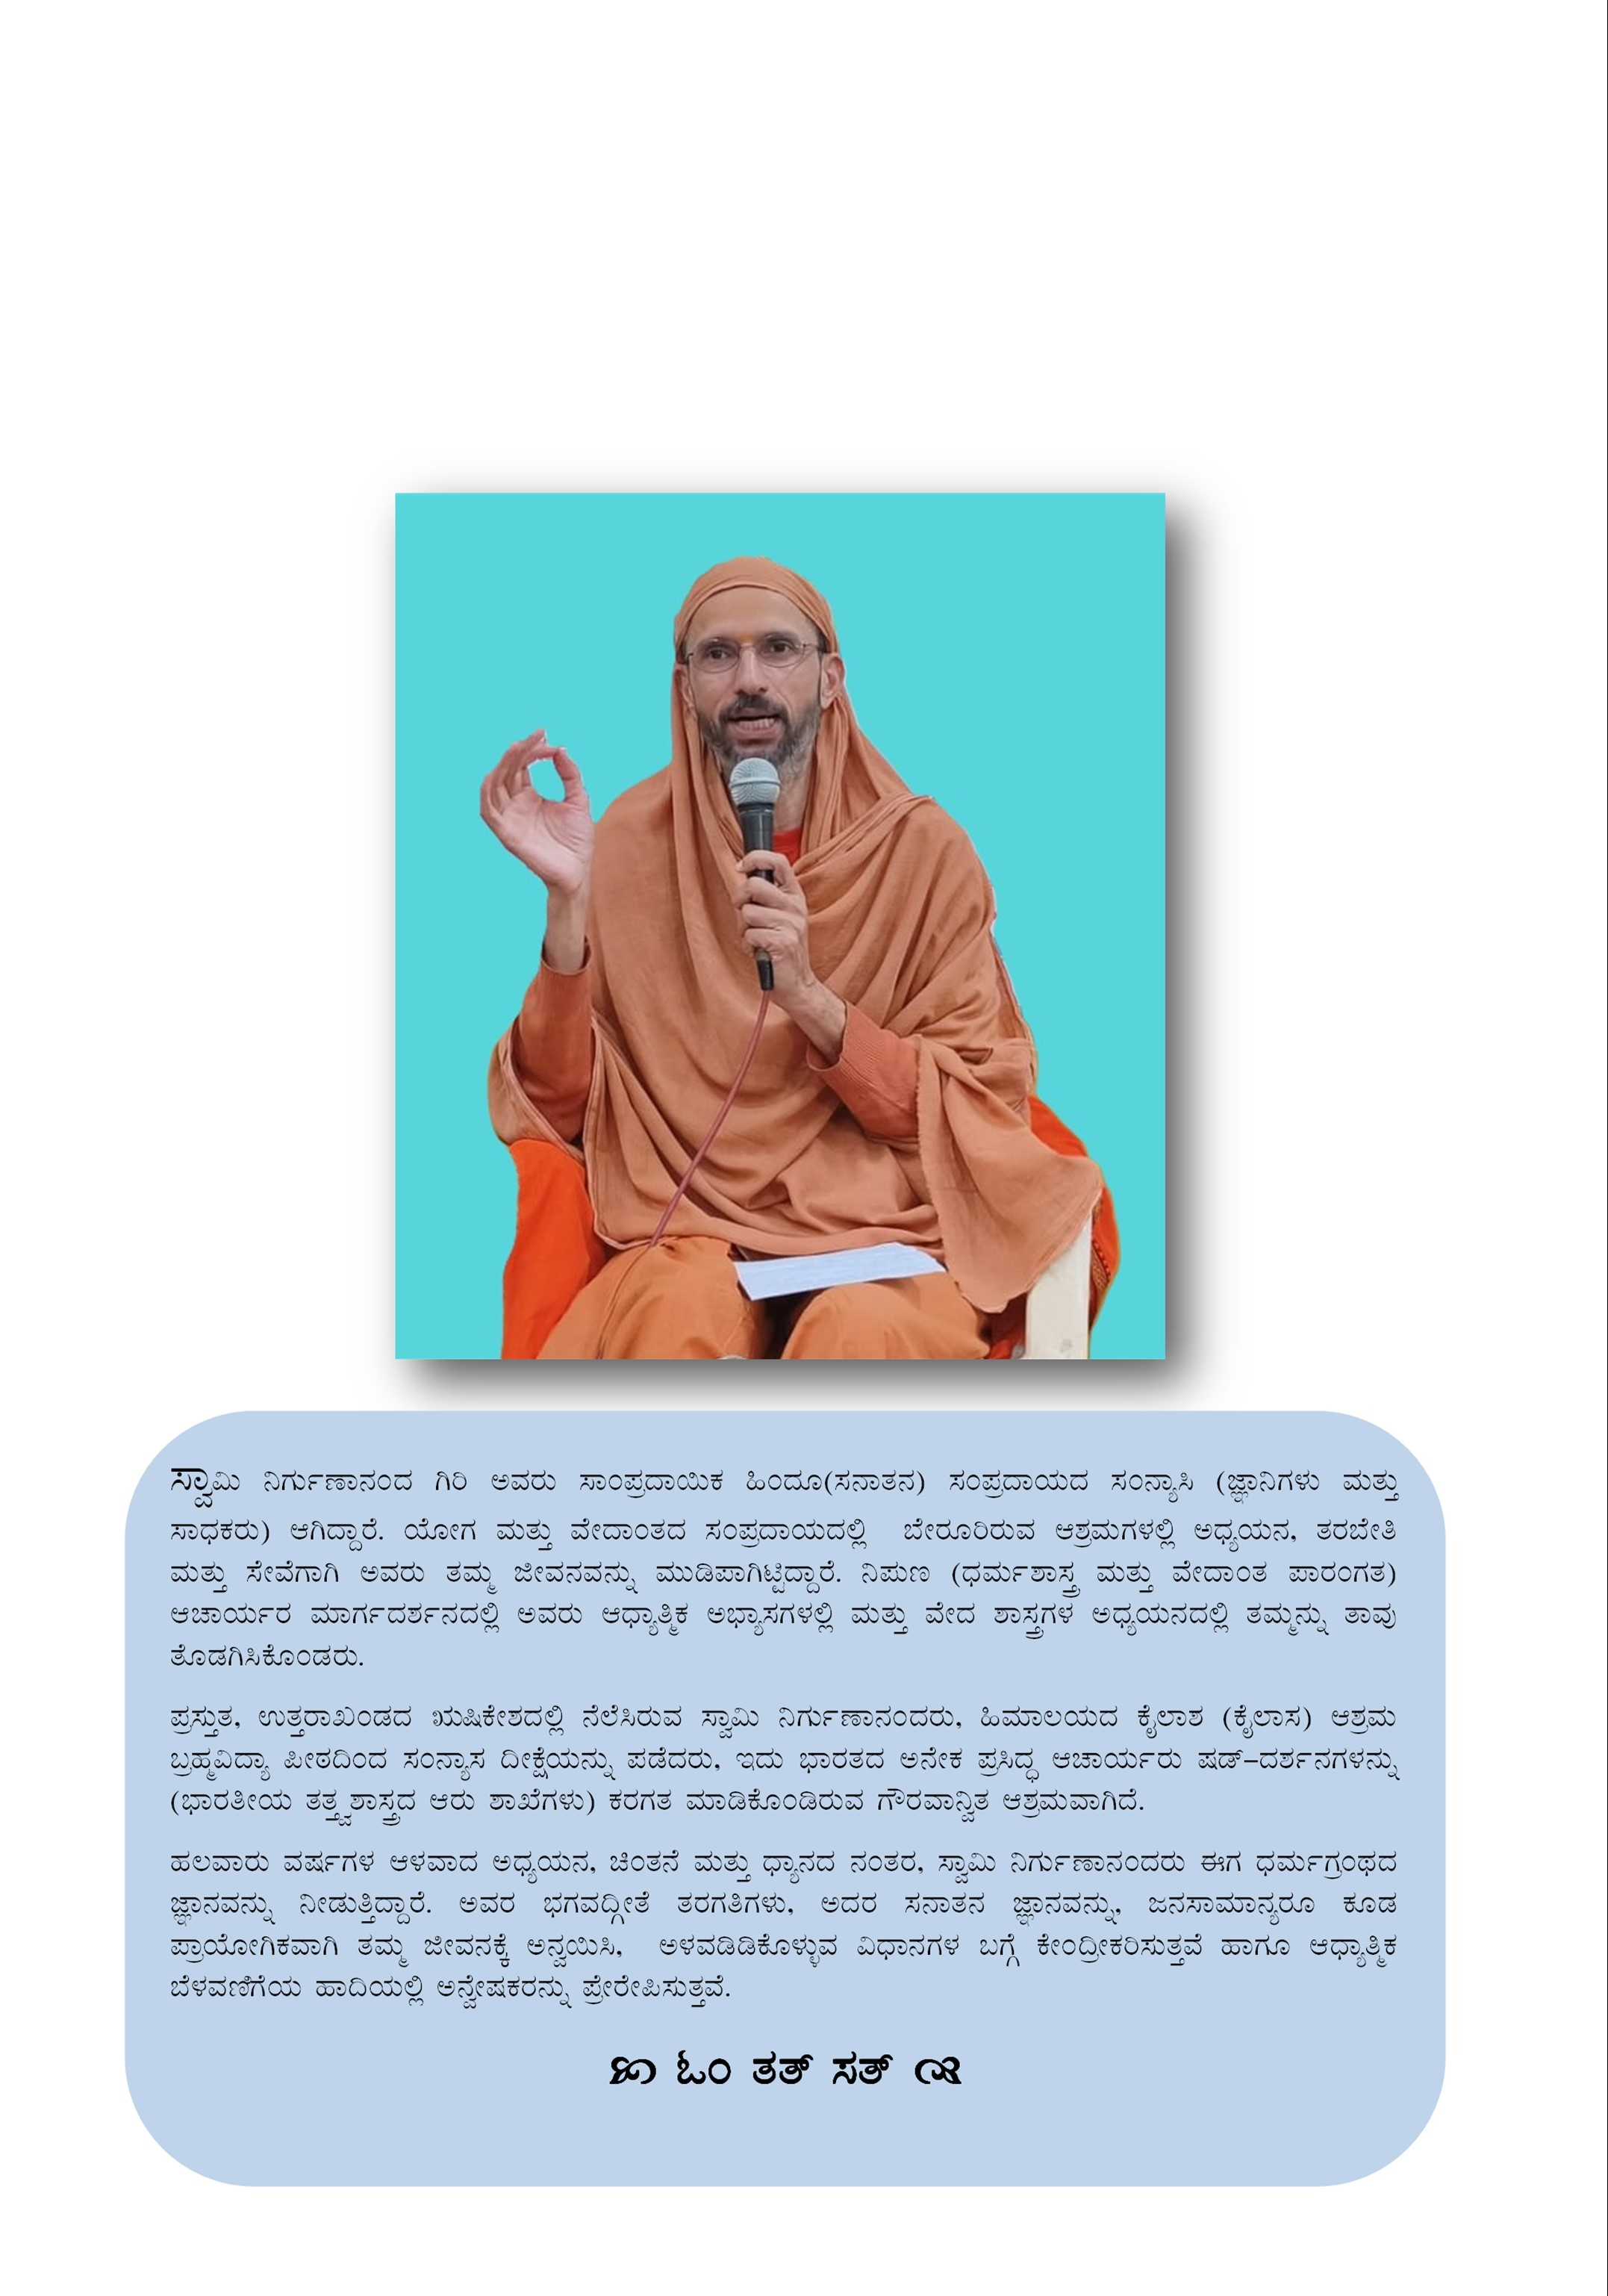
\includegraphics[width=\paperwidth,height=\paperheight]{./images/page02.jpg}%
    }%
	}
   \else% do nothing
   \AddToShipoutPictureBG*{%
    \AtPageLowerLeft{%
        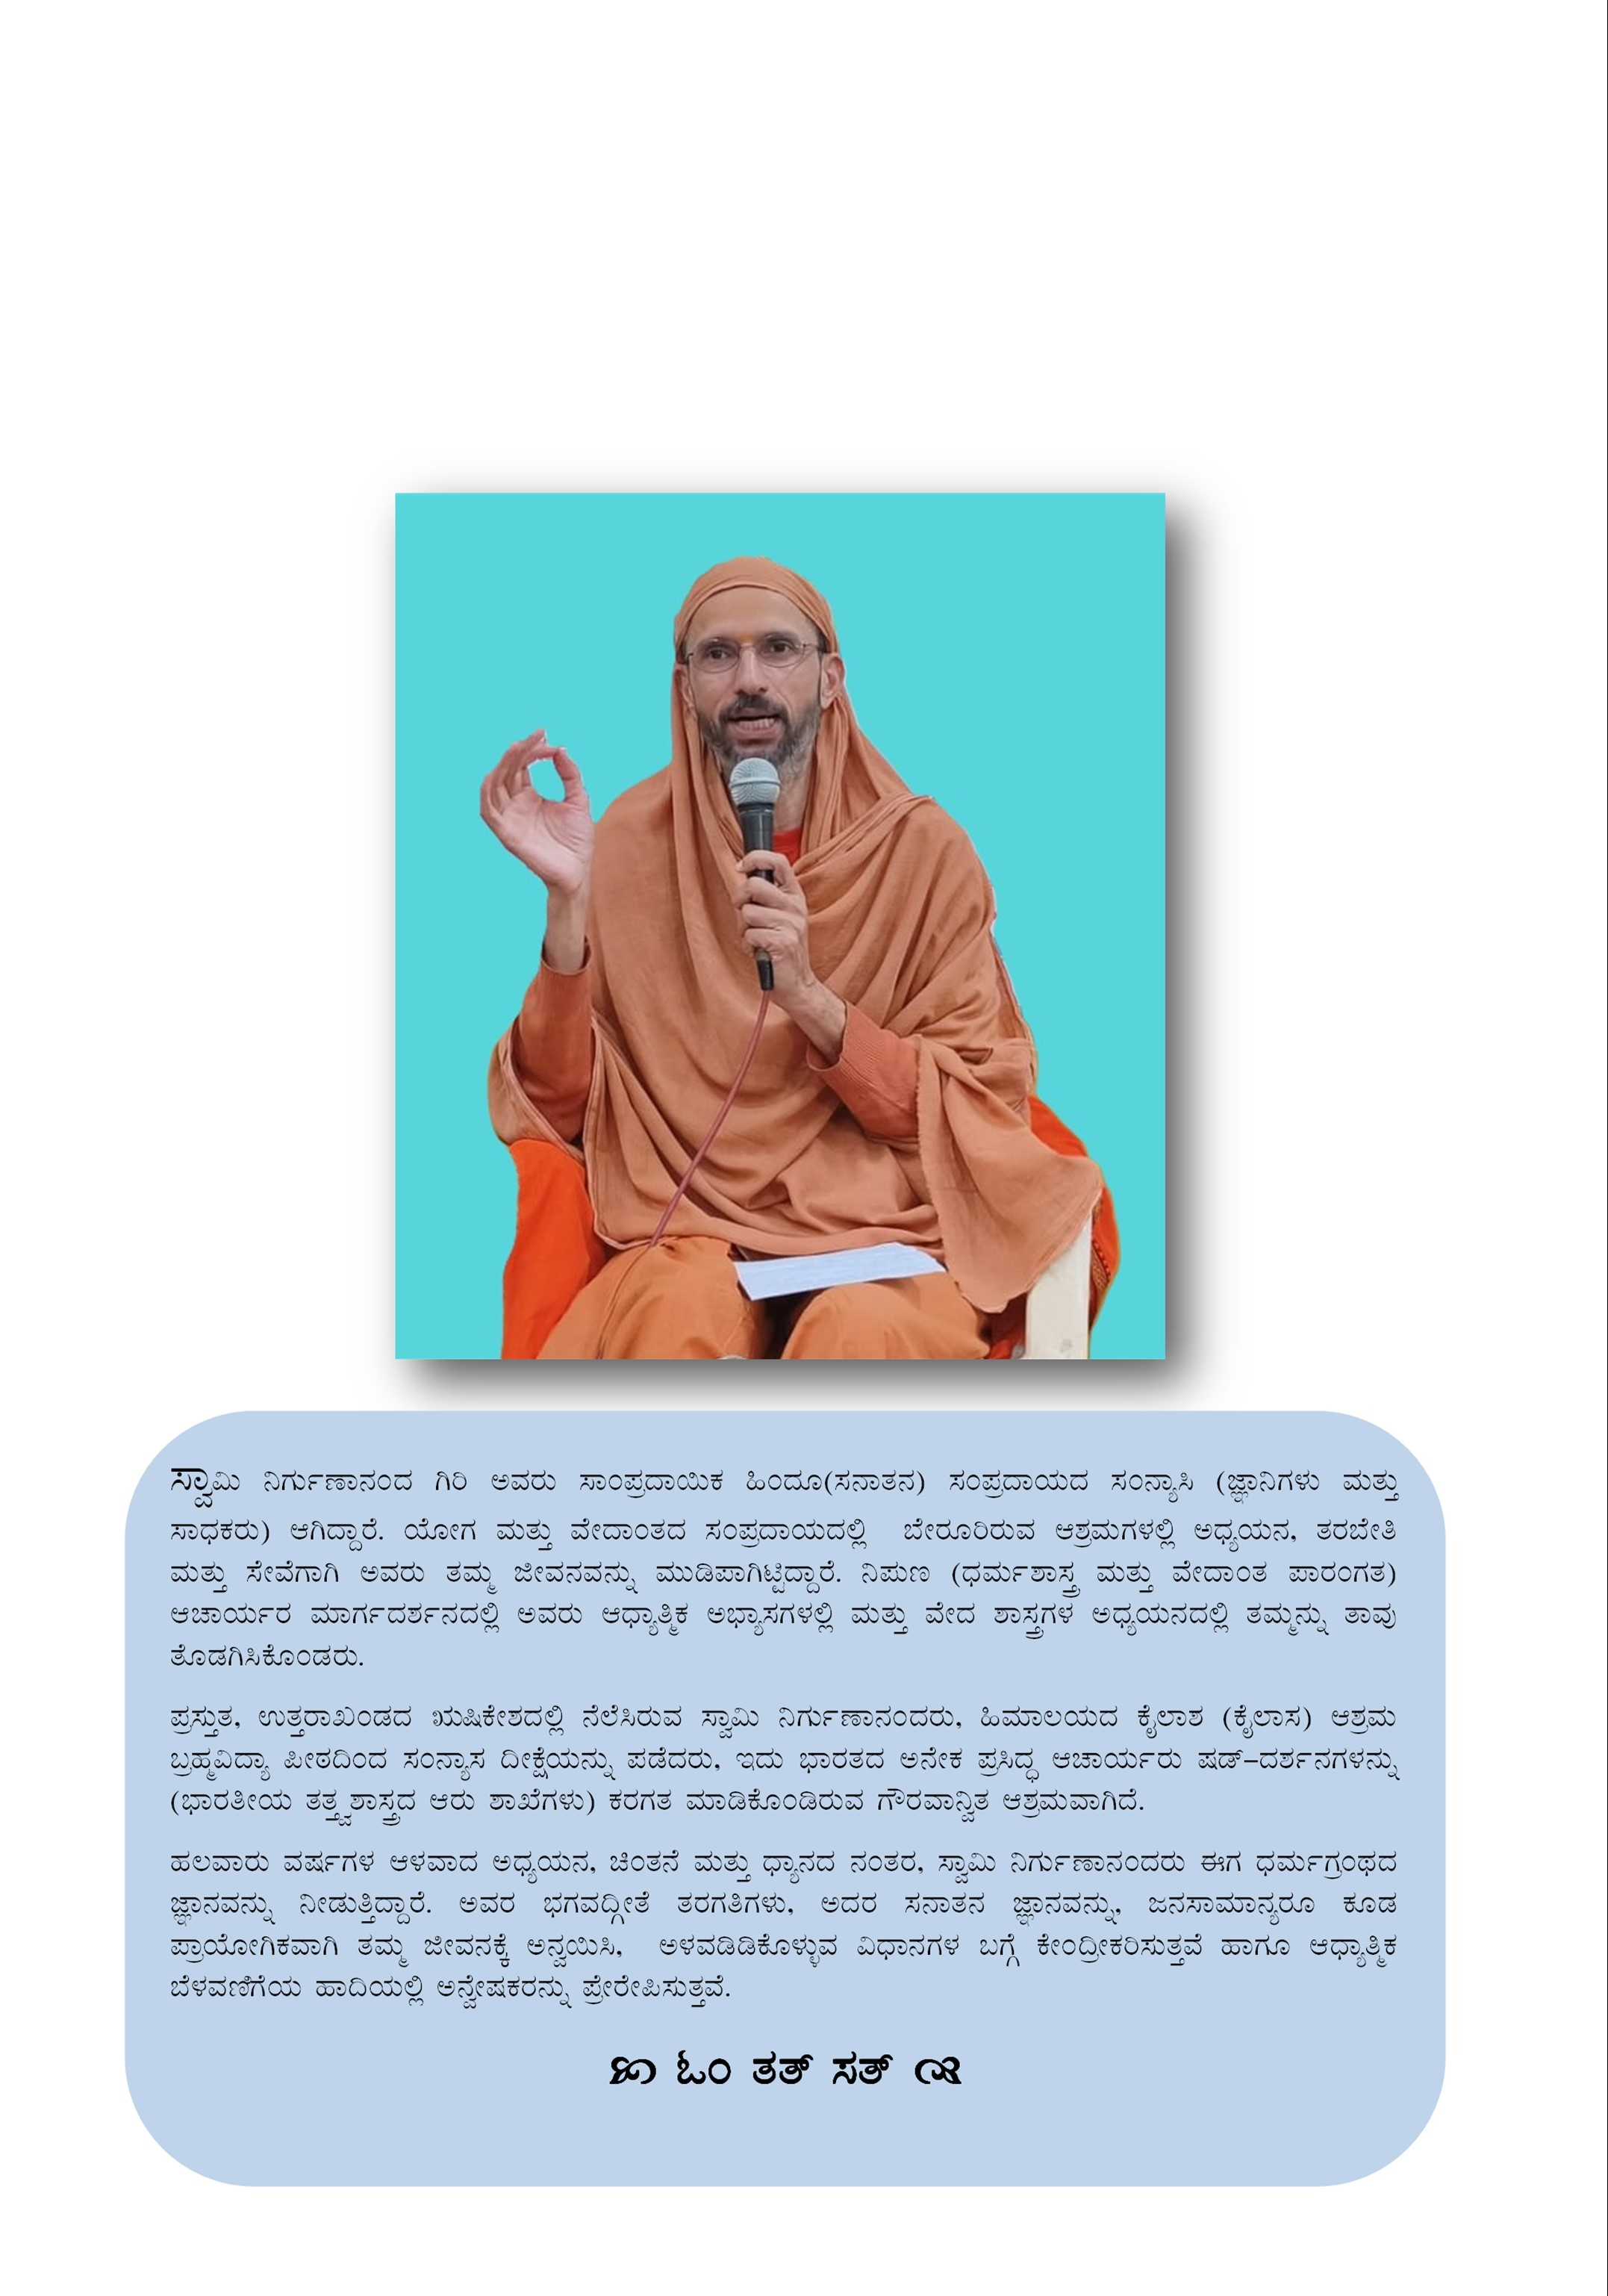
\includegraphics[width=\paperwidth,height=\paperheight]{./images/page02.jpg}%
    }%
	}
\fi
\begin{titlepage}
	%\pagecolor{pastelblue}
	\AddToShipoutPictureBG*{%
    \AtPageLowerLeft{%
        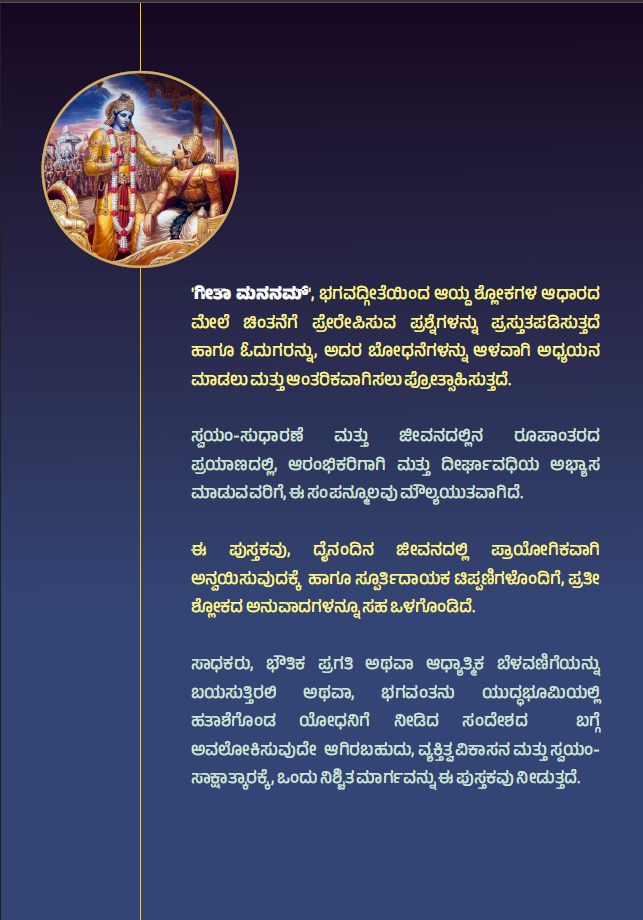
\includegraphics[width=\paperwidth,height=\paperheight]{./images/backcover.png}%
    }%
}
    \begin{center}
        \vspace*{0.5cm}
            
        {\Huge
        %\textbf{\color{white}\fontsize{50}{60}\selectfont ಗೀತಾ ಮನನಂ}
		}
        %\textbf{\\ \small \color{white}ದೈನಂದಿನ ಸ್ಪೂರ್ತಿ ಹಾಗೂ ಆತ್ಮಾವಲೋಕನಕ್ಕಾಗಿ}    
        \vspace{1.0cm}
            
        
		
            
        \vfill
            
        
            
        \vspace{0.1cm}
        {\color{white}    
		%\textbf{{\Large \mananamfont ಸ್ವಾಮಿ ನಿರ್ಗುಣಾನಂದ ಗಿರಿ}}\\
		%{\normalsize Swami Nirgunananda Giri\\Rishikesh, India}
        }
    \end{center}
\end{titlepage}
\nopagecolor% Use this to restore the color pages to white
\end{document}
